\documentclass[12pt,letterpaper,twoside,openright,oldfontcommands]{memoir}
\usepackage{ucvpsitesis}
\usepackage[spanish]{todonotes}
\usepackage{booktabs, tabularx, multirow}

\addbibresource{tesis.bib}
\author{Leonardo Pérez \\ & & Emerson Yancul}
\tutor{Luisana Gómez}
\departamento{Psicología Social}
\mail{leo.prez.k@gmail.com; eyanor@gmail.com}
\date{Caracas, junio de 2018}
\title{Identidad de género y transición en las personas transgénero de Caracas}
\shorttitle{Identidad de género y transición}
\engtitle{Gender identity and transition on transgender people from Caracas}

\begin{document}
    \maketitle
    \nocite{*}
    \frontmatter
    % \chapter{Agradecimientos}
%
% \chapter{Dedicatoria}

\chapter{Resumen}
\begin{center}
	\large\scshape\thetitle\
\end{center}

\begin{quote}
\small
La investigación tuvo como fin explorar la construcción de la identidad de un
grupo de personas transgénero que hacen vida en la ciudad de Caracas. Se empleó
una metodología cualitativa con perspectiva fenomenológica, basándose en el
estudio de casos. La recolección de datos se realizó a través de entrevistas a
profundidad, las cuales fueron realizadas a adultos mayores de 18 años de ambos
sexos que se identifiquen a sí mismos como transgénero y fueron codificadas
empleando el programa informático ATLAS.ti\@. Dicha codificación dio como
resultado 6 categorías que constituyen los elementos esenciales que permiten la
construcción de identidad en los participantes. Se pudo observar que la
identidad de estas personas se encuentra mediada en gran parte por la
interacción con otros individuos. La transición es una herramienta de
reafirmación tanto personal como social de la propia identidad de género. La
transición se vive como un continuo que tiene como fin último ser cissexual,
aunque se acepte que no existe actualmente la capacidad técnica viable para
lograr ese objetivo. Por ello la persona transgénero despliega un conjunto de
estrategias secundarias para compensar y lograr aproximarse lo más posible a la
expresión de género que consideran apropiada para su identidad. La
discriminación juega un papel de obstáculo que afecta el desarrollo de la
identidad de las personas transgénero.
\end{quote}

\itshape\textbf{Palabras clave:}\normalfont{}\ Transición, transgénero,
transexualidad, género, identidad, discriminación, desarrollo, cuerpo,
expresión de género.

\chapter{Abstract}

\begin{center}
	\large\scshape\theengtitle\
\end{center}

\begin{quote}
\small
This research had the intention of exploring the construction of
transgender's identity that live in the city of Caracas. A qualitative
methodology with a phenomenological perspective is used, by way of case
study. Data collection was done through in-depth interviews, which were
conducted to adults over 18 who identify themselves as
transgenders. Interviews were codified using the software ATLAS.ti\@. This
coding resulted in 6 categories that constitute the essential elements that
allow the construction of identity in transgender people. We found that their
identity is largely mediated by the interaction with other individuals.
Transition is a tool used to reassure their own gender identity both
personally and socially. This transition is experienced as a continuum whose
ultimate goal is to become cissexual, while accepting that this is not
currently technically possible. For this reason, transgender people make use
of a set of secondary strategies to compensate and approximate their desired
gender expression according to their identity. Discrimination plays a major
role as an obstacle that encumbers the development of identity in transgender
people.
\end{quote}

\itshape\textbf{Keywords:}\normalfont{}\ Transition, transgender, transsexual,
gender, identity, discrimination, development, body, gender expression.

    \cleardoublepage\tableofcontents
    \clearpage\listoftables*
    \listoffigures*
    \mainmatter\chapter{Introducción}
% Miércoles 19 de julio de 2017
El sexo, el género y la identidad sexual no carecen de investigación.
Todo un cuerpo investigativo se ha desenvuelto desde el inicio de los
movimientos de derechos para las mujeres.
Este discurso y forma de concepción de las diferencias de género se ha
constituido en un lenguaje de circulación común.
A su vez ha sido modelado por el activismo político a partir del surgimiento del
feminismo de segunda ola \parencite{Helfrich2001}.
Alrededor del género circulan discursos que defienden ciertos ordenamientos
sociales y formas de interacción.
El acceso efectivo a campos sociales enteros (como son propuestos por
\textcite{Bourdieu1992}) puede ser definido en función del género de una
persona.
Y las formas de explicar, justificar y definir el género tienen el potencial de
hacer prevalecer hegemónicamente algunos tipos de ordenamientos sobre otros.

Esto ha generado cambios sociales en las formas de considerar y construir el
género.
Estos cambios son, sin embargo, dispares entre distintos grupos culturales,
clases y campos sociales.
Estudiar estos cambios y las diferencias que existen permitirá complejizar la
comprensión del género y brindar herramientas de intervención.
La población de personas transgénero ha sido tradicionalmente invisibilizada.
Usualmente se les agrupaba junto con homosexuales y se les consideraba a todos
conjuntamente como enfermos mentales.
Igualmente existía en el imaginario la noción de que los hombres homosexuales
querían ser mujeres o que las mujeres homosexuales deseaban ser hombres.
Con estas concepciones se confundían dos posturas de identidad que hoy en día se
entienden de forma separada \parencite{MejiaTurizo2010-06}.

Cuando inició el movimiento de reconocimiento de la diversidad sexual se comenzó
a reconocer la diferenciación entre algunas categorías.
Estas se tratan de la diferenciación entre: sexo genético, sexo genital,
identidad sexual, identidad de género, expresión de género y orientación sexual.
Esto ha llevado al surgimiento de nuevas categorías y a cambios en la forma en
la cual se entiende la identidad sexual y de género
\parencite{Figari2010,Bleichmar2006}.

Sin embargo, esta se trata de la comprensión académica desde los estudios de
género.
En la sociedad en general prevalecen otros imaginarios y otras posturas.
El rechazo a la unión entre personas del mismo sexo, a la posibilidad de
adopción son caras visibles del problema.
Pero aún no se reconoce ni se conversa abiertamente.
Sobre el cambio de género y de sexo, existen muchísimos malentendidos y mitos
rodeando una condición que la misma academia científica no es capaz de
comprender en su totalidad aún \parencite{Bleichmar2006}.

Como resultado de lo anterior existe aún un rechazo, a veces abierto y a veces
encubierto, ante aquellas personas que deciden cambiar de sexo o que deciden
vivir de acuerdo a un rol de género distinto al que se le asignó al nacer.
Este problema no es visible entre aquellos que logran mostrarse exitosamente
como el género que desean o entre aquellos que no inician aún esfuerzos para
mostrarse como ese género.
Sino que se hace frontal y visible para aquellos que apenas están iniciando una
transición de sexo o, en algunos casos, cuando desean mostrarse según su género
deseado pero aún no lo logran de manera exitosa.
Esto usualmente resulta en una estigmatización social de la persona transgénero
o transexual.

La comprensión de la transexualidad puede ser, entonces, una herramienta
fundamental para afrontar la discriminación, rechazo y estigmatización que
sufren las personas transexuales o transgénero. Si bien existe una tradición de
investigación experimental alrededor de los fenómenos de exclusión social y
estigmatización, también es cierto que otras perspectivas menos psicologicistas,
como las teorías performativas, sugieren que existen un amplio componente de
deseabilidad social e interacción que determinan el rechazo activo o pasivo de
algunas categorías y grupos sociales. De ello se puede intuir que un análisis de
las interacciones y prácticas que estructuran al género hoy en día puede dar una
mejor comprensión y brindar o sugerir nuevas estrategias para la inclusión
social.

Lo anterior vislumbra una de los elementos centrales de la importancia del tema
del género y la transexualidad. Muchas de las elaboraciones en psicología y
sociología tienen su origen en fenómenos y estudios del siglo pasado. Sin
embargo, el cambio social no se detiene y siempre el cambio de las teorías y
paradigmas en la academia será mucho más lento que los cambios sociales. Es
importante entonces mantener una vigilancia constante sobre aquellos temas que
se creen cerrados o terminados en cuanto a su comprensión teórica. Igualmente,
se han evidenciado cambios importantes y diferencias significativas en las
formas de comprensión de la masculinidad y la feminidad durante las pasadas
cuatro décadas. Estos cambios no son obvios ni pueden darse por sentado pues el
cambio social no es uniforme ni homogéneo. Es decir, no se da en todos los
lugares simultáneamente, ni se da de igual manera. Venezuela tiene una inserción
muy particular dentro de la dinámica de la cultura occidental, con vastas
variaciones y aproximaciones a las realidades sociales. Las diferencias de
clases y de campos en nuestro país son distintas a aquellas de otros países. No
es entonces transferible directamente la interpretación de estos cambios
culturales, sin ser tampoco completamente ajeno a las influencias. En particular
desde el surgimiento de la comunicación instantánea mediante Internet y el
fenómeno de las redes sociales virtuales. Es de valor entender estos cambios en
Venezuela. Permite ubicarnos dentro de un ámbito que está cambiando rápidamente
en el mundo. Y además que tiene el potencial de afectar nuestra dinámica
social. Los roles de género y las dinámicas de interacción entre ellos forman una
parte fundamental de la forma en la que se estructura una cultura y una
sociedad. Tiene impacto en prácticas, creencias, imaginarios y representaciones.
Por tanto es deber de la academia científica poder hacer seguimiento de este
fenómeno y dar cuenta de los cambios históricos y su interacción con otros
fenómenos.

De particular importancia es la inserción que tienen las personas transexuales
en los servicios de atención médica para la transición de un sexo a otro. Debido
a que el cambio de sexo es el aspecto central del criterio para la definición de
la transexualidad separada de otras expresiones alternativas del género tales
como el ser transgénero y la expresión queer.

\todo{Verificar el orden de las descripciones a capítulos en este segmento}
Es por ello que el presente trabajo de investigación está compuesto de un
marco referencial ubicado en el Capítulo II, donde se realiza una definición
sobre género, seguido de una breve reseña histórica del transgénero o
transexualidad, seguido por apuntes históricos sobre el mismo en Venezuela.
Luego se explica de manera concisa como es visto el transgénero y la
transexualidad desde las perspectivas: biologicista, sociológicas, psicológicas
y patologización. Posteriormente, se describen conceptos que vienen a
representar el eje central de la investigación entre los que destacan identidad,
autopercepción y la mirada del otro.

Seguidamente en el Capítulo III  se describe el planteamiento del problema, este
en resumen, señala que ante la incógnita que representa la construcción de la
identidad trans desde una mirada psicológica no clínica, se plantea la
exploración de las vivencias de las personas trans para poder dar respuesta a las
siguientes preguntas de investigación: ¿Cuál es el lugar de la transición de
sexo en la construcción de la identidad de género de los transexuales de
Caracas?, ¿cómo acceden, utilizan y se insertan en los servicios médicos de
transición de sexo estas personas?, ¿qué lugar ocupa la transición de sexo en su
vida cotidiana?

Estos aspectos llevan a reflexionar acerca del transgénero o transexualidad como
un campo de estudio de suma amplitud y complejidad, por lo que resulta necesario
analizarlo desde una perspectiva psicosocial, y no conformarse con la
interpretación del sentido común que se tiene al respecto. La perspectiva de una
persona transgénero o transexual sobre las diferentes dimensiones del mismo es
muy relevante, desde el porqué de la elección de esta forma de vida, la decisión
de soportar la mirada a veces despectiva del otro y correr los riesgos de los
prejuicios.

En el capítulo IV, se esbozan los objetivos que rigen el estudio para dar
respuesta a la pregunta de investigación. En el Capítulo V se plantea una
investigación de tipo cualitativa, con enfoque fenomenológico, mediante el
empleo de entrevistas a profundidad, con el propósito fundamental de conocer y
aprehender el fenómeno desde la perspectiva de cada participante, en
concordancia con la pregunta y objetivos planteados.

En el capítulo VI se analizan los contenidos construidos en las entrevistas,
generando así, de acuerdo a los hallazgos, unas unidades de análisis.
    \section{Planteamiento del problema}

La transexualidad y el transgenerísmo son temáticas que nunca ha sido
investigada en la escuela de psicología. Esto incluye a la mención de psicología
social, en donde la temática apenas ha sido tocada tangencialmente en algunas
elaboraciones sobre el género.

Actualmente la temática que parece dominar el discurso desde la psicología
social, en otras partes del mundo, es el asunto de la patologización de la
transexualidad\footnote{La transexualidad suele ser el único fenómeno estudiado
o mencionado debido a la prevalencia del discurso biologicista y médico en la
psiquiatría. Este considera innecesario conversar sobre el transgenerísmo bajo
la concepción de que en este no existe una ‘disforía de género’. Al no haber
patología no hay necesidad de acción. Sin embargo, se ignora que el
transgenerismo puede ser una etapa previa a la transexualidad si se dan los
procedimientos de transición necesarios para cumplir con la clasificación.
Revisar los conceptos relevantes en la página~\pageref{diferencia}}. En
particular la paradoja que se encuentra en conjunto con los requerimientos
legales para realizar la transición de sexo. La situación actual en Venezuela se
desconoce. Por ello decidimos realizar un estudio de las percepciones,
imaginarios y concepciones que existen alrededor del transgenerismo en
particular en relación los procedimientos de transición de un sexo a otro.
Para ello partimos de dos artículos recientes. El primero trata de un
planteamiento realizado por \textcite{Coll-Planas2015} en el que visibilizan el
uso estratégico que es dado por parte de las personas transexuales de la
patologización como medio para acceder a los procedimientos de transición.

En su revisión del contexto médico y jurídico de España encuentran que, la
perspectiva de los servicios que ofrecen los procedimientos de transición de
sexo sobre la transexualidad, conlleva una carga negativa, binarista,
biologicista y patologizante que obliga, en el caso de los transexuales
masculinos, a una reproducción exagerada de los estereotipos de la masculinidad
hegemónica. Es decir, debido a que:

\begin{quote}
[…] se refuerza la idea de que lo natural y lo sano es que el sexo (nacer en un
cuerpo de macho o de hembra,) la identidad de género (sentirse hombre o
mujer) y el rol o la expresión de género (actuar de forma masculina o
femenina) estén articulados de un modo normativo \parencite[][p.
426]{Coll-Planas2015}.
\end{quote}

Se hace entonces necesario que la persona transgénero reproduzca los roles de
género de forma incluso más estricta y punitiva que lo que se esperaría de una
persona no trans.

Este punto nos hace pensar que existe una presión estructural social sobre la
persona trans para alterar su expresión de género y proyectar, no de la forma en
que ellos lo harían espontáneamente en otra circunstancia, sino de la forma que
se les exige para poder acceder a la transición. \textcite{Coll-Planas2015}
explican que:

\begin{quote}
[…] desde el modelo hegemónico[, binarismo masculino y femenino,] se pone
énfasis en normalizar a las personas trans para que reproduzcan un género
normativo, lo que incluye la presión para la transformación corporal ya que […]
la modificación de las características sexuales es crucial para fundar la
masculinidad y la feminidad en una base biológica \parencite[][p.
427]{Coll-Planas2015}.
\end{quote}

El segundo artículo consultado es una investigación realizada en Bogotá,
Colombia, por \textcite{LassoBaez2014}. En la misma se realizaron varias
entrevistas a profesionales psicólogos y psiquiatras, así como a personas trans,
acerca del tema de la transición y los servicios médicos utilizados para
realizar la misma. Uno de los aspectos resaltantes es que, desde su punto de
vista, se hizo necesario consultar tanto a las personas que acuden a los
servicios de salud como a los psicólogos y un psiquiatra que atiende a estos
usuarios. Esto los lleva a tener dos puntos de vista alrededor de una sola
realidad que pueden ser contrastados en función de los conceptos centrales.
Aunque se menciona el papel y la relación que tienen otros actores, como
enfermeras y personal administrativo, sólo se toma en cuenta la construcción que
hacen de ellos los entrevistados.

Allí encontraron, mediante un análisis crítico del discurso como es propuesto
por VanDijk (citado en~\cite[][p. 111]{LassoBaez2014}), que una de las fuentes
más fuertes de discriminación, en la forma de micro agresiones y trato
prejuicioso, provienen del personal auxiliar de los servicios de salud. En menor
medida, entre los profesionales de atención es donde se presenta con más
frecuencia el desconocimiento de la transexualidad y falta de estrategias para
proveer atención de calidad a esta población. Encontraron, además, con la
patologización de la transexualidad con una doble función paradójica. Pues
permite, simultáneamente, el acceso a los servicios de transición, así como un
elemento de discriminación y vulneración de la identidad y expresión de la
persona trans.

Esto ubica un poder sobrevalorado a la opinión clínica de los médicos.
\textcite{LassoBaez2014} señala: “en la práctica psiquiátrica es común que el
certificado de \emph{disforia de género} sea negado cuando la experiencia de la
persona no responde a los criterios de feminidad y masculinidad del profesional”
(p. 122). Por esta razón, lo que termina sucediendo es que se fuerzan los
estereotipos de género sobre la identidad de la persona trans que requiere
atención médica. Es por ello que Lasso Báez concluye que “Esta situación lleva a
muchas personas […] a mentir en las entrevistas psiquiátricas, exagerando
ciertos rasgos e hipervigilando su comportamiento para ajustarse a estereotipos
de género” (p. 122).

Ambas investigaciones apuntan a un rol preponderante de la
transición en la construcción de la identidad transexual y transgénero.
En particular cuando se desea transitar de un sexo a otro mediante
procedimientos seguros ya que existen muchos riesgos asociados a esta
transición. Por esto las personas transgénero se ven forzadas a lidiar con las
visiones hegemónicas de la medicina sobre el sexo y el género para poder acceder
a estos procedimientos. Siendo los principales métodos: a) la terapia de
reemplazo hormonal, que requiere la prescripción de una toma de hormonas de
parte de un especialista endocrinólogo; b) la mamoplastia o cirugía de senos, ya
sea mamoplastia de aumento o mastectomía, extirpación de la glandula mamaria y
reducción del volumen del seno; c) la cirugía de reasignación de sexo, en la
cual se transforman los genitales existentes para ajustarlos un sexo u otro.

Esta situación es merecedora de atención en el contexto venezolano donde parecen
prevalecer con fuerza los estereotipos de género machistas y no se ha conducido
investigación desde la psicología social para comprender el fenómeno del
transgenerísmo y la transexualidad en nuestra cultura.

En función de abordar este vacío, realizamos la presente investigación que busca
dar respuesta a la pregunta planteada en la página~\pageref{preguntas}.

	
%¿Cuál es el lugar de la transición de sexo en la construcción de la identidad
%de género de los trans de Caracas?

\section{Objetivos}
Para dar respuesta a la pregunta de investigacion planteada presentamos los
siguientes objetivos de investigación.
Estos objetivos articulan el alcance de la investigación y la forma en la nos
aproximaremos a la pregunta de investigación.

\subsection{Objetivo General}
	\begin{itemize}
		\item Comprender la transición y la construcción de la identidad de las
		personas Transgénero que hacen vida en el Área Metropolitana de Caracas.
	\end{itemize}

\subsection{Objetivos específicos}
	\begin{itemize}
		\item Identificar los elementos centrales de la constitución de la identidad
	de género de un grupo de personas trans masculinos de Caracas.
		\item Identificar los elementos centrales de la constitución de la identidad
	de género de un grupo de personas trans femeninos de Caracas.
		\item Identificar las modalidades y estrategias que utilizan las personas
	transexuales de Caracas para acceder a los procedimientos de transición de sexo.
	\end{itemize}

    % 	
%¿Cuál es el lugar de la transición de sexo en la construcción de la identidad
%de género de los trans de Caracas?

\section{Objetivos}
Para dar respuesta a la pregunta de investigacion planteada presentamos los
siguientes objetivos de investigación.
Estos objetivos articulan el alcance de la investigación y la forma en la nos
aproximaremos a la pregunta de investigación.

\subsection{Objetivo General}
	\begin{itemize}
		\item Comprender la transición y la construcción de la identidad de las
		personas Transgénero que hacen vida en el Área Metropolitana de Caracas.
	\end{itemize}

\subsection{Objetivos específicos}
	\begin{itemize}
		\item Identificar los elementos centrales de la constitución de la identidad
	de género de un grupo de personas trans masculinos de Caracas.
		\item Identificar los elementos centrales de la constitución de la identidad
	de género de un grupo de personas trans femeninos de Caracas.
		\item Identificar las modalidades y estrategias que utilizan las personas
	transexuales de Caracas para acceder a los procedimientos de transición de sexo.
	\end{itemize} % Fijados, objetivos definitivos
    \section{Justificación}
% TODO Revisar refencias de la justificación
El interés y la preocupación social por el acoso, invisibilización y prejuicio
hacia una persona transgénero va en aumento. El interés y la preocupación social
por el acoso, invisibilización y prejuicio hacia una persona transgénero va en
aumento. Como aparece reflejado en portales de noticias, como El Mundo, para
el 2016 ya un 80\% de la pobblacion trans (bien sea transexual o transgénero)
han vivido situaciones de discriminacion o agresiones \parencite{Alpuente2016}.


% Según Fernández, Guerra, Díaz y Grupo GIDSEEN (2014) “este hecho se debe a actos graves tales como
% depresión, ataques y suicidios de las partes afectadas a consecuencia de sufrir
% acoso por parte de sus compañeros o incluso de su propia familia” (p. 32).

Para poder adentrarse dentro de lo que significa la transexualidad o el
transgenerismo es necesario cimentar el interés de la presente investigación en
base a la noción de que la construcción de la identidad es un hecho influenciado
por factores psicosociales. Esto es planteado por autores como Paramo (2008) que
expresa que los individuos sufren una fuerte influencia del medio en el que se
desarrollan al momento de construir su identidad. Hecho que no es consciente,
sino un resultado de interacciones, es decir, un individuo que se vea rodeado o
se desenvuelva en una cultura en la que el hombre tiene unas características
particulares va a asumir estas como elementos constitutivos pero también su
propia interacción con otros miembros de su comunidad podría afectar el tipo de
hombre o mujer que llegue a ser.

 Existe una progresiva concientización sobre la importancia de los derechos
 humanos y sobre la educación acerca de este tema en espacios tan vulnerables
 como el colegio, la universidad, transporte público, lugar de trabajo, entre
 otros \parencite{Fernandez2014a}.

Investigaciones sobre las consecuencias, incidencias, factores, características
y todo tipo de variables del fenómeno \emph{bullying} han incrementado con el
fin de conocerlo mejor para la elaboración de instrumentos de evaluación y su
respectiva intervención. Estos tipos de acosos son generalizados, es decir,
afectan indiferentemente del país o clases sociales. “A menudo se asocia de
manera exclusiva el transgenerismo con el mundo adulto como si la identidad de
género fuera únicamente fruto de un largo proceso de introspección personal
resuelto al cabo de muchos años” (Fernández et al., 2014 p. 32).

Éste mismo autor, hace referencia a que la realización de una intervención por
parte de los asistentes sanitarios correspondientes es de vital importancia,
pues “se debe preparar y enseñar a la sociedad conceptos éticos y morales,
enseñar a las personas a actuar delante de situaciones de acoso, burla o abuso y
a intervenir delante del primer síntoma” (Fernández et al., 2014, p. 34).

El transgénerismo según Mejía y Almanza (2010) “se manifiesta típicamente en la
medicina y la psiquiatría por una identificación intensa y persistente con el
otro sexo, con un sentimiento de inadecuación con el sexo asignado, y por un
deseo permanente de vestir, vivir y ser tratado como miembro del otro sexo” (p.
91). Las personas transgénero consideran que han nacido en un sexo equivocado.
La mayoría, refiere el inicio de los síntomas desde la primera infancia.

El concepto de género nació para designar todo aquello que es construido por las
sociedades para estructurar y ordenar las relaciones sociales. Al basarse estas
construcciones sociales y simbólicas en la diferencia sexual, se estructuran
relaciones de poder cuya característica esencial es el dominio masculino. La
dominación masculina se fundamenta en la diferencia sexual, la cual se explica
por el diferente lugar que ocupa cada sexo en el proceso de reproducción, idea
también del pensamiento judeocristiano. Se instaura así la lógica del género,
que parte de una oposición binaria: lo propio del hombre y lo propio de la mujer
(lo esencial en la feminidad y la masculinidad), y dicha lógica del género es
una lógica de poder, de la dominación del sistema patriarcal (Mejía y Almanza,
2010).

La persona transgénero es mal vista en la sociedad. Debido a la discriminación
dirigida hacia los transexuales y transgénero este grupo de personas
experimentan sentimientos de vergüenza de que se descubra su identidad de
género. Además deben enfrentar circunstancias en las que son calificados como
mentalmente enfermos. Dar pasos para expresarse de acuerdo a su identidad les
ocasiona sentimientos de culpabilidad en función del rechazo social. Deben
ocultar su verdadera identidad y en ocasiones incluso se les exija que esté de
acuerdo con los otros y pretenda condenar sus propios intereses y actividades,
como en los rituales de reafirmación del rol de género.

Esta doble vida de la persona transgénero, antes de decidir presentarse como su
identidad de género, es en ocasiones llevada con miedo, puede ser difícil de
mantener y también puede conducir a trastornos mentales como la depresión. El
transgénerismo es una condición fundamental en la construcción de la
personalidad de la persona trans, y su expresión permitirá el ingreso o no a
diversos campos dependiendo de los capitales con los que cuente. Pero las
actitudes de las demás personas hacia esta condición crean una situación de
tensión que también afecta del desarrollo de la personalidad y puede también
impedir la integración efectiva de las personas trans en la comunidad.

Una gran proporción de personas transgénero son incapaces de adaptarse a las
presiones y se convierten en bajas sociales. Estos son los trans que se
encuentran con mayor frecuencia en las calles prostituyéndose. Ahora que se
estableció que los transgénero no son fisiológicamente diferentes, también
existe la posibilidad que poco a poco la sociedad sea más tolerable en cuanto a
su respeto y no discriminación (Sáez, 2006).

    % Miércoles, 9 de mayo de 2018
\chapter{Marco referencial}\label{ch:marcoreferencial}
Para poder realizar una aproximación adecuada a la pregunta de investigación
el primer requisito es dar cuenta del estado actual de la comprensión
científica de la transexualidad y la transgeneridad.
Para ello haremos una exposición breve de los conceptos más importantes que
se ven involucrados en la construcción de la identidad desde el concepto
mismo del género hasta la autoimágen corporal.
Incluyendo varias exploraciones respecto al devenir histórico y científico
del entendimiento de lo trans, investigaciones previas y diversas teorías
explicativas que rodean a este tema.

\section{Género}

Para poder adentrarnos en el tema que es el foco de la presente investigación es
necesario primero realizar una revisión de lo que es el género.
Aunque a primera vista eso podría parecer un tema relativamente sencillo, no se
debe tomar a la ligera, pues como lo indica Lamas (1999) el emplear la palabra
género conlleva implicaciones históricas, en un primer momento el feminismo
académico anglosajón usó este término para diferenciar las construcciones
sociales y culturales, pero esto probó ser complicado pues dio pie a que
surgieran una variedad de formas de interpretación, simbolización y organización
de las diferencias relacionadas con la sexualidad y el sexo complejizando de
esta manera la concepción inicial y la aplicación que se le había dado al
concepto de género.

Sin embargo, Lamas rescata una propuesta realizada por Scott (1996 c.p.~Lamas
1999) la cual plantea que el género posee dos
partes, analíticamente interrelacionadas aunque distintas, y cuatro elementos.
Lo central de la definición es la “conexión integral” entre dos ideas: el género
es un elemento constitutivo de las relaciones sociales basadas en las
diferencias que distinguen los sexos y el género es la forma primaria de
relaciones significantes de poder.
Con esto en mente es posible que establezcamos una primera característica para
poder adentrarnos en lo que significa el género, y esta sería que está
determinada por las relaciones sociales y las diferencias que se asignan según
el sexo (biológico) de las personas.

Se puede también rescatar lo propuesto por Bourdieu (2000) cuando se refiere
al hecho de que la socialización y la construcción de los géneros ha sido
históricamente demarcada y delimitada por la biologización de lo social, para
generar una división arbitraria de lo que implica haber nacido con un sexo y
tener impuesto un género y unos roles en base a este determinante biológico.
Este autor se adentra en esto planteando que las diferencias visibles entre los
cuerpos se convierten en el factor determinante para promover una visión
androcéntrica del mundo, dando así significados y valores particulares según sea
el caso.

Entonces, para comprender el significado de la palabra \emph{Género} es
preciso tener en cuenta que en los últimos quince años los trabajos
realizados han mostrado cuánto varían las categorías de género con el tiempo y
% TODO cuales trabajos?
con ellas los territorios sociales y culturales asignados a mujeres y hombres.
En muchos períodos históricos las percepciones populares acerca de los
% TODO cuales períodos?
temperamentos masculino y femenino han sufrido cambios sustantivos, que han
venido acompañados por un nuevo mapa de las fronteras sociales (Scott, 1996).

El concepto de género como se mencionó en párrafos anteriores, fue introducido
por feministas estadounidenses en la década de los sesenta para plantear la
reflexión sobre los sexos.
En la próxima sección exploraremos los orígenes precisos del término en los
experimentos de John Money.

Por su parte la autora Huggins (2005) señala que no sólo somos seres sexuados,
sino portadores de cultura y de necesidades que son atravesadas por nuestras
condiciones y experiencias de vida.
Por lo cual se debe ir más allá del dato biológico sexo cuando se analiza la
categoría del género, ya que esta “se desprende de manera tal que, en sus
contenidos, es cada vez más social” (p.~18), haciéndose necesaria la clara
distinción entre sexo y género.

\begin{quote}
    Que sea masculino o femenino no puede ser juzgado de la misma manera: los
    criterios serán culturales, por lo tanto, diferentes según el tiempo y el
    lugar.
    El sexo debe ser admitido como constante, pero también debe admitirse la
    variabilidad del género (Oakley, 1972; c.p.~Muñoz, 2004, p. 17).
\end{quote}

Lo que esta perspectiva pretende explicar es que aquellas características y
actitudes que usualmente son tomadas como \emph{atributos naturales} de los
hombres y de las mujeres, no son necesariamente determinadas por la biología,
sino que son construidas socialmente.

En esos ámbitos de discusión, lo correspondiente al sexo se presenta como un
conjunto invariable de características biológicas y, en cierta medida, termina
suponiendo que ese sexo biológico es la base natural de una asignación cultural
del género, la cual determinaría las conductas y los roles que pueden ocupar
hombres y mujeres en cada sociedad.

Es importante destacar que los sistemas de género (sin importar el período
histórico) son sistemas binarios que oponen la hembra al macho, lo masculino a
lo femenino, rara vez sobre la base de la igualdad, sino, por lo general, en
términos jerárquicos.
Si bien las asociaciones simbólicas con cada uno de los géneros han variado
enormemente, han incluido el individualismo versus la crianza, la razón versus
la intuición, lo construido versus lo naturalmente procreativo, la ciencia
versus la naturaleza, la explotación versus la conservación, lo clásico versus
lo romántico, la universalidad de los rasgos humanos versus la especificidad
biológica, lo político versus lo doméstico, lo público versus lo privado.
Lo interesante en estos contrastes es que privan procesos sociales y culturales
mucho más complejos, en los que las diferencias entre mujeres y hombres no son
ni aparentes ni tajantes, y es en ello que reside su poder y relevancia (Scott,
1996).

\subsection{Diferencia entre Sexo y Género}
El origen de la distinción entre sexo y género surge en 1949, cuando Simone de
Beauvoir (1998 c.p.~Butler, 2010) en su libro \emph{El Segundo Sexo}, afirma “no
se nace mujer: se llega a serlo” (p.~89)
Pero es John Money (c.p.~Buttler, 2010), quien menciona la palabra género por
primera vez.
De esta manera se inicia la discusión sobre una diferencia que había sido
naturalizada, la distinción entre lo que es el sexo y el género, que ha sido
tema de discusión desde entonces en las ciencias sociales.
El primero se refiere al hecho biológico y a las características físicas de los
cuerpos, mientras que el segundo se refiere a los significados que cada sociedad
atribuye a esa diferenciación y que definen lo que es el género.
Este concepto describe el modo en que se organizan los sexos en su relación
social, por lo que implica siempre una relación, que es además una relación de
poder, donde la distinción por géneros vendría a ser parte de nuestra
\emph{naturaleza} tanto comportamental como de los espacios sociales que están
asignados a cada persona según su sexo, como también de acuerdo a su edad,
etnia, clase social, entre otras cualidades que puede tener una persona, y que
permite la restricción y clasificación de su acceso social (Beauvoir
c.p.~Butler, 2010).
De esta forma, se encuentran distintas definiciones de sexo, como la de la
Organización Mundial de La Salud (en Villegas, Rodríguez y Ochoa, 2002) que lo
asume como:

\begin{quote}
    Una distinción por las características biológicas o fisiológicas asociadas
    típicamente con hembras o machos de una especie.
    Es la condición orgánica que distingue a las hembras (mujeres) de los machos
    (hombres).
    El sexo biológico es la anatomía sexual junto con los cromosomas de cada
    persona.
    Biológicamente o se nace hombre o se nace mujer (p.~84)
\end{quote}

Otra definición la plantea Almuneda (2007) quien menciona que, a pesar de que el
“sexo” parezca un concepto aséptico, biológico y sin posibilidad de matización,
se sabe desde los estudios de John Money (c.p.~Almuneda, 2007), a mediados
de los años 50, que tiene una determinación multivariada, siendo necesario para
la determinación del sexo de un bebé, la combinación de cinco componentes
biológicos:

\begin{itemize}
    \item \emph{Sexo genético}: determinado por los cromosomas X e Y.
    \item \emph{Sexo hormonal}: el balance estrógenos-andrógenos.
    \item \emph{Sexo gonadal}: presencia de testículos u ovarios.
    \item Morfología de los órganos reproductivos internos.
    \item Morfología de los órganos reproductivos externos.
\end{itemize}

Sin embargo, la experiencia de John Hopkins (c.p.~Almuneda, 2007) en su trabajo
% TODO determinar John hopkins o john money
con bebés, condujo a éste psiquiatra a utilizar el término “género” a partir de
1955 para plantear que el psiquismo de un nuevo ser, adquiere una orientación
distinta masculina o femenina dependiendo de si se trata de un hombre o una
mujer, esto se adquiere a través de las interrelaciones que establece con el
entorno social durante los primeros dos o tres años de vida.

Los estudios de género han seguido la línea del planteamiento de Hopkins,
pues, lo que entendemos por género no debe entenderse en el simple sentido de
contemplación desinteresada sino, como plantean Fonseca y Quintero (2009), que
es totalmente político el sentido de la distinción de géneros.
El género no es asumido sólo para la clasificación y distinción de las personas,
sino que más allá de ello se encuentra que en la clasificación existe un
elemento de control y restricción, y un posicionamiento de poder que genera
discriminación en cuanto a lo que no se encuentra bajo la heteronorma
\footnote{Cathy Cohen (2005) define la heteronormatividad como la práctica y
las instituciones “que legitiman y privilegian la heterosexualidad y las
relaciones heterosexuales como fundamentales y naturales dentro de la
sociedad”. Según Rich (1980) La heteronorma o heteronormatividad
es un régimen social, político y económico que impone las prácticas sexuales
heterosexuales mediante diversos mecanismos médicos, artísticos, educativos,
religiosos, jurídicos, etc.\ y mediante diversas instituciones que presentan
la heterosexualidad como necesaria para el funcionamiento de la sociedad y como
el único modelo válido de relación sexoafectiva y de parentesco.
El régimen se retroalimenta con mecanismos sociales como la marginalización,
invisibilización o persecución.
Tiene como base un sistema dicotómico y jerarquizado.
Esto incluye la idea de que todos los seres humanos se distribuyen en dos
categorías distintas y complementarias: varón y mujer;
que las relaciones sexuales y maritales son normales solamente entre personas de
sexos diferentes;
y que cada sexo tiene ciertos papeles naturales en la vida.
Así, el sexo físico, la identidad de género y el papel social del género
deberían encuadrar a cualquier persona dentro de normas íntegramente masculinas
o femeninas.}
y los patrones hegemónicos de lo que representa cada sexo en cada cultura.
Existen múltiples estudios de género desde la antropología
% TODO ejemplos de esos múltiples estudios
precisamente para distinguir entre el sexo biológico y el género como un
constructo social, precisando así, el papel de la construcción sociocultural en
la que se interviene en el mundo subjetivo de cada persona que al nacer, además
de un nombre adecuado a su género, luego debe ser instruido con patrones
distintivos para poder comprender el mundo social al cual va a ser inserto.

Este mundo social además de tener sus propios códigos de género, también en el
ejercicio del control social, asigna papeles asimétricos en el ejercicio de
poder de dichos roles.
Estas estructuras asimétricas no nacen de un vacío social, sino que surgen como
una identidad a partir de los procesos psicosociales.
De esta forma, algunos autores plantean que las interpretaciones de género
% TODO algunos quienes?
residen en lo biológico y lo corporal, es decir, sitúan la clasificación como un
asunto propio de la naturaleza biológica
Pero en la Teoría de los roles sexuales planteada por Fagot (1982) se sostiene
que la interpretación del rol se relacionaba con la estructura definida por la
diferencia biológica, la dicotomía entre lo masculino y lo femenino, y no con
una estructura definida por las relaciones sociales (Connell, 2003 c.p.
Botello, 2005).
Durante muchos años se consideró la masculinidad y la feminidad como una única
dimensión, con dos polos, que hacía posible clasificar a los individuos en un
determinado punto de ese continuo, es decir, éstos podían ser en mayor o menor
grado masculinos o femeninos, pero nunca las dos cosas a la vez.
Asimismo, los roles sexuales estaban rígidamente ligados al género, de manera
que el ser masculino o femenino dependía básicamente de ser hombre o mujer
(Kohlberg, 1996).

En la década de los setenta, “ha surgido una nueva concepción que considera
la masculinidad y feminidad como dos dimensiones independientes, de tal forma
que todos los individuos poseen en mayor o menor grado esos dos rasgos”
(Spence y cols, 1975, p. 29).
Así, ha nacido el concepto de androginia psicológica, para designar a aquellos
individuos que presentan en igual medida rasgos masculinos y femeninos, y se han
desarrollado una serie de cuestionarios y escalas específicas para medir la
masculinidad, feminidad y androginia.
En este nuevo enfoque de los roles sexuales, la masculinidad y feminidad
“representan dos conjuntos de habilidades conductuales y competencias
interpersonales que los individuos, independientemente de su sexo emplean para
interactuar con su medio” (Spence y cols, 1975, p. 35).

Esta perspectiva ha posibilitado el desarrollo de numerosas investigaciones, al
disminuir considerablemente la inevitabilidad y el determinismo ligado a los
rasgos masculino y femenino (Spence y cols, 1975).
Por su parte Lagarde (s.f.,\ c.p.~García, 2000), tiene planteamientos más
fundamentales sobre la conformación de los géneros, para ella:

\begin{quote}
    Son formaciones políticas que están estructuradas a partir de cargas y
    tensiones de poder que aseguran a los sujetos sociales cumplir sus deberes
    como mujeres y como hombres, y les impiden, al mismo tiempo, realizar
    las prohibiciones.
    Sus objetivos centrales son: a) Especializar a los sujetos definidos a partir de
    su sexo;
    b) convertirlos en expertas/os, en actividades y funciones particulares
    que los hagan ser mujeres y hombres;
    y c) lograr la continuidad del mundo así estructurado.
    Así, a través de variados mecanismos los sujetos quedan incluidos o excluidos de
    ámbitos y relaciones, y ocupan posiciones jerárquicas.
    Además, a las funciones y a las actividades asignadas se les confiere valor
    económico, social y cultural, que se convierte en poderío o en carencia de
    poderes, para mujeres y hombres, y para la sociedad.
    Así, la organización genérica asegura determinada distribución de poderes y de
    bienes que permite preservar el orden del mundo (p.~77).
\end{quote}

Con una estructura social categorizada y clasificada, se facilita el control
social, por lo que otros autores buscan la distinción entre el sexo y el género
para generar un planteamiento ante lo naturalizado y así contribuir a la
comprensión de la complejidad de lo que se construye socialmente como
masculinidad.
Buenfil (1985 c.p.~Botello 2005), en sus planteamientos feministas, similares
a los de Lagarde, asume que el género no es lo único que genera identidad en la
persona, sino que sus actividades sociales, laborales, la pertenencia a un
estrato social, el nivel de escolarización, entre muchas otras característica
van asignando un lugar social en el que se define al individuo y que dichas
características aseguran un lugar en la sociedad a la persona, a estos
planteamientos la autora los denomina “Polos de Identidad”, que describen a los
individuos dentro de continuos bipolares para definir su identidad.

Es importante rescatar, que tanto el sexo como el género son elementos que a lo
largo del desarrollo de la humanidad han marcado y direccionado las relaciones
entre los individuos y consecuentemente permiten dar sentido a los
cuestionamientos que se puedan presentar cuando se interpelan discursos que
naturalizan conductas o actos dentro del mundo social que se vean como propios
de la biología de un hombre o una mujer.
Pues, el discurso de género como había sido tratado, había sido un núcleo para
definir y clasificar a las personas, que se construye a través de un proceso de
socialización que distingue el sexo a través de lo biológico, y que también
ubica a éste discurso desde un puesto de poder de las ciencias básicas, lo que
implica que situar éste discurso desde la ciencia tiene también una carga
política.

De manera tal, que en el mundo la noción de género (antes de la intervención de
la teoría de género) se había reducido burdamente a su componente biológico,
naturalizando su carga social, que determina nociones, relacionales sexistas
promovidas socioculturalmente, que generan identificación, justificación de
conductas, encubrimiento de discriminaciones, entre otros, ahora tiene otras
posibles resignificaciones y reconstrucciones (Lizardo, 2008).

\subsection{Identidad de Género: Masculinidad, Feminidad y Trans}
El discurso social que interpretamos sobre las relaciones de género tiene sus
condiciones de existencia sobre la constitución de las identidades masculinas y
femeninas, con una modalidad excluyente que se construye en relación con una
división sexual del trabajo, fundada en la separación de la vida social entre
una esfera de lo público (producción) y otra esfera de lo privado
(reproducción), y la asignación de los hombres a la primera y de las mujeres a
la segunda (Cubillán, 2012).

La identidad puede entenderse como el auto-reconocimiento y pertenencia que
experimenta un individuo particular.
Siendo estos elementos los que caracterizan al sujeto o a la colectividad frente
a los demás.
La identidad también puede considerarse como la conciencia que una persona tiene
respecto a sí misma y que la convierte en alguien diferente a los demás.
A pesar de que muchos de los rasgos que conforman la identidad son hereditarios
o innatos, el entorno ejerce gran influencia en la conformación de la
especificidad de cada individuo (Hothersall, 2004).

Por otra parte, la Identidad de Género hace referencia básicamente al
auto-reconocimiento como niño o niña, hombre o mujer, mientras que la
identificación implica sentimientos de suplencia, deseos de ser como otro.
La tipificación sexual o asunción del rol que la sociedad asigna a cada sexo es
distinto de ambos conceptos, ya que se trata de asimilar las características
conductuales propias de cada sexo en una sociedad determinada (Hothersall,
2004).

Thompson (1975) hace una distinción fundamental que ha permitido clarificar este
campo de discusión, ya que definen la Identidad de Género como la
auto-clasificación como hombre o mujer, basada principalmente en la figura
corporal;
y el Rol Sexual, por otra parte, hace referencia a “los comportamientos,
sentimientos, actitudes que se consideran propios de un hombre
o una mujer, teniendo entonces una base más cultural” (p.~76).

El mismo autor refiere que la adquisición de la identidad y rol sexual ocurre
entre el año y medio a los tres o cuatro años.
Primero el niño aprende a reconocer que hay dos sexos, luego se incluye a sí
mismo en una u otra categoría, y a partir de aquí comienza a usar el rotulo del
sexo como guía de referencia relacionada con los roles sexuales.
La permanencia de género se adquiere a los seis o siete años.
Esta permanencia no tiene en un principio su origen en los genitales como podría
esperarse, sino que está más relacionado con las características del rol.
Existe un período posterior en el que el género está determinado por los
genitales en lugar de por las conductas dependientes del rol (llevar el cabello
de una u otra forma, usar vestidos, etc.).
A este periodo llegará el niño hasta los siete o nueve años (Thompson, 1975).
Es necesario aclarar que desde el momento en que este autor realizo sus
propuestas a la actualidad han surgido nuevas teorías que nutren la comprensión
de la identidad de género.

Vedrell (2009) afirma que la Identidad de Género no se trata exclusivamente de
la biología sino que incluye factores sociales, contextuales y psicológicos, por
lo que el entorno social y los valores relacionados a lo masculino y femenino en
una sociedad determina y en gran parte condiciona las conductas y actitudes
generando un modelo a seguir, el cual está basado en estereotipos e ideales.
Por esta razón, todo lo que no esté dentro de los estándares de normalidad
sexual pasa a ser anormal o patológico.

\subsubsection{Masculinidad}
Toda persona es validada según su hacer, una persona cuyo hacer no es propio
actúa en detrimento de sí misma y entonces se encuentra alienada, una
explicación para esto es lo que los escritores Hegel y Marx definen como la
alienación, un fenómeno que puede ser entendido como la extrañación o la
desapropiación.
Para estos teóricos “una persona está alienada cuando es de manera distinta,
ajena, extraña a cómo debería ser” (Catilla, 1986 c.p.~Lizardo, 2008).
Entre estos fenómenos alienantes se encuentra la noción de que el género y el
sexo son elementos estáticos determinados por características biológicas como
por ejemplo la carga genética (noción que es errada pues el género se encuentra
determinado por factores socioculturales mientras que el sexo si podría
encontrarse influenciado por elementos genéticos), es en estas situaciones
cuando la incorporación de elementos que rompen con la norma llevan a la
alienación del individuo y en este caso específicamente podría plantearse que la
ruptura con la alienación a la hetero-norma, crea malestar en la forma
individual de vivirse.

Resulta importante reconocer la visión masculina para la comprensión de los
malestares que gestan la masculinidad hegemónica.
Los estudios de género empiezan a incorporar al hombre a partir de los años 90,
lo que permite ampliar la visión del concepto y no sólo el estudio de lo
femenino o la mujer (Cubillán, 2012), y en este sentido el mayor énfasis por el
estudio para la comprensión de lo masculino ha recaído principalmente sobre las
mujeres, sumando en su mayoría a mujeres estudiando lo femenino y mujeres
estudiando lo masculino, aportando mayor investigación desde lo femenino según
relata Botello (2005).

El mundo de la masculinidad se describe dentro de un mundo social más complejo,
donde existen otros roles y otras categorías definitorias de la persona, lo que
evidencia que el espectro de género es complejo.
Como hace referencia Butler (2010) “la categoría “mujer” no puede describirse
con características hegemónicas, tampoco la masculinidad puede definirse como
una única forma de ser, y aunque en su manifestación de poder sigue conservando
un lugar privilegiado en el mundo social” (p.~106).
Es necesario reconocer que la conformación de la masculinidad está articulada
con otras estructuras sociales, donde conjuntamente participan en la elaboración
de contenidos simbólicos que orientan la organización social y que asignan un
lugar privilegiado al hombre, pero no a cualquier hombre, sino aquel que cumple
con unas características especiales en cuanto a etnia, posición económica y
orientación sexual (Botello, 2005).

De acuerdo a Burín (2003) en la actualidad factores como la clase, raza y
orientación sexual se han convertido en determinantes de la diferenciación
masculina es por esto que en palabras de la autora, existen distintas
masculinidades.
Esto no es algo descabellado pues como ya lo hemos expresado anteriormente la
construcción de la masculinidad es un proceso que viene determinado por las
interacciones del sujeto con otros individuos del mismo género así como con
individuos del género contrario.
Es entonces aquí donde se encuentran construcciones sobre lo que significa ser
hombre tan variadas como hombres hay, consecuentemente la construcción de un
hombre único con el que se pueda identificar un individuo es bastante difícil.

Autores como Téllez y Verdú (2011) afirman que:

\begin{quote}
    El “hacerse hombre” puede ser considerado un proceso de construcción social en
    el que se le asigna a lo masculino una serie de características definidas por la
    sociedad que tienen como finalidad mantener la experiencia exclusiva del poder a
    aquellos individuos masculinos (p.~80).
\end{quote}

Sumado a esto, los autores plantean que por medio del estudio de la masculinidad
se puede revelar un sistema en el que el género actúa como medio de control e
imposición de actividades sobre los individuos de una población.
Además es necesario remarcar que, en palabras de Téllez y Verdú (2011), la
concepción de lo que se considera que es masculino ha variado según factores
como el momento histórico, la etapa evolutiva, el nivel socioeconómico, entre
otros.

Las autoras también hacen énfasis en que a la masculinidad suele exigírsele una
expresión más activa.
Es decir, se debe demostrar ser hombre según tu etapa de desarrollo.
Tomando todo esto en cuenta se podría reafirmar la noción de que no existe una
forma única y correcta de lo que significa ser hombre, ya que la masculinidad
está construida en base a aspectos sociales y que los mismos no son estáticos e
inmutables.

\subsubsection{Feminidad}
Para el autor Martínez-Herrera (2007):

\begin{quote}
    La historia oficial es escrita por el hombre que asume la representación
    universal de la humanidad;
    otra muy diferente es la historia de las mujeres.
    Lo masculino y lo femenino constituyen producciones sociales en un momento dado,
    por lo cual no están exentas de tensiones y se encuentran siempre en movimiento
    (p.~88).
\end{quote}

El mismo autor considera que:

\begin{quote}
    Los hombres y las mujeres reproducen, aunque no inevitablemente a nivel onto y
    filogenético la perpetuación de estas condiciones.
    A pesar de los profundos cambios estructurales en la esfera de la producción, la
    ideología y las leyes, acaecidas a través de los tiempos, estas condiciones se
    mantienen relativamente invariables.
    La perduración de las condiciones vejatorias femeninas cuyo origen se pierde
    en los albores del tiempo humano, nos lleva a la pregunta acerca de cuáles son
    los procesos subyacentes a dicha constante histórica (p.~88).
\end{quote}

El género ha sido históricamente conceptuado sobre la base de parámetros
masculinos.
En la antigüedad lo femenino, era establecido por oposición a lo masculino, es
su negativo o el reverso.
Lo femenino es lo que no es, o lo que no se debe ser, un lugar proscrito que
convoca el horror o el rechazo.
De hecho, al rival se le deshonra asemejándolo a una mujer.
La feminidad se erige así, como un antivalor determinado por la exclusión y no
como un valor intrínseco a partir de sus propias características y naturaleza.
De lo anterior se concluye que el sexo femenino es un no-sexo o dicho en otras
palabras, es un sexo que no le pertenece a la mujer (Irigaray, 1977).

Para Martínez-Herrera (2007):

\begin{quote}
    La teoría feminista brinda como corpus teórico polisémico algunas claves para
    la comprensión del problema de la reproducción de las condiciones históricas de
    la discriminación femenina, derivándose diversas explicaciones en dos órdenes.
    Uno a nivel de las relaciones de poder omnipresentes en la teoría de género y
    otro que alude a la constitución y la construcción del género como atribución
    cultural, personal y psicológica (p.~89).
\end{quote}

Ambas dimensiones se entrecruzan y se multideterminan entre sí.
Concretamente Scott (1996) dice que:

\begin{quote}
    […] tres han sido los enfoques teóricos privilegiados en los análisis del
    género, a saber: un esfuerzo específicamente feminista por explicar el
    patriarcado;
    un intento de compromiso de la tradición marxista con las críticas feministas;
    y la tradición psicoanalítica en dos de sus vertientes fundamentales, la
    denominada teoría de las relaciones objétales y el estructuralismo freudiano
    francés.
\end{quote}

En general, las distintas explicaciones y teorizaciones coinciden en la
existencia de dos constantes históricas como elementos determinantes en la
construcción social de la feminidad, una de ellas es lo que Bourdieu (2000 c.p
Martínez-Herrera, 2007) denomina:

\begin{quote}
    El cuerpo de la mujer como capital simbólico, en tanto objeto de apropiación
    y deseo, como cuerpo para el otro.
    Por otra parte, tenemos a la mujer/madre, siempre al servicio y cuidado de los
    demás.
    La mujer se debate así entre dos representaciones sociales disociadas entre sí,
    la maternidad a ella asignada y el erotismo que remite a la mujer a una
    condición primigeniamente sexual/genital (p.~89).
\end{quote}

Para Lagarde (1997 c.p.~Martínez-Herrera, 2007), históricamente:

\begin{quote}
    La feminidad está atravesada por una dimensión óntica de ser para otros, que es
    donde adquiere sentido vital y reconocimiento de sí, por su contribución a la
    realización de los demás.
    Ésta condición remite a la mujer a una permanente incompletud y la
    ubica al servicio de una ética de cuidados, encargada de dar,
    preservar, proteger y reproducir la vida (p.~89).
\end{quote}

La ubicación de la mujer en una esfera no tradicional supone romper con el ideal
estereotipado de mujer-madre y la coloca en el sospechoso lugar de trasgresión,
lo cual funciona como una fuente de represión social y psicológica
(Martínez-Herrera, 2007).

Por su parte, Burín (2003) además de adentrarse en el tema de la subjetividad
masculina también toca principalmente la subjetividad femenina, la cual al igual
que el caso de la masculina viene determinada por aquellas interacciones que
tiene un individuo y que le permiten construir un ideal de feminidad, el cual no
puede estar ligado a una concepción fija de lo que es el ser.

Además de lo anteriormente mencionado, Martínez- Herrera (2007) reafirma que
históricamente el género se ha presentado en un continuo.
No es sólo una construcción social sino que también actúa como filtro cultural
que permite acercarse e interpretar de una manera particular al mundo.
Con esto en mente se podría entender entonces que la experiencia masculina y la
femenina suelen colocarse en extremos opuestos y con connotaciones particulares.

Es por esto que se asume al hombre como representante universal de la humanidad
a diferencia de las mujeres.
Para Lagarde (1997 c.p.~Martínez-Herrera, 2007), quien hace referencia a la
feminidad, la propone como algo que históricamente ha sido concebida en función
de ser para otros, es decir, la imagen de mujer que ha sido construida se ha
enfocado en que su existencia adquiere sentido y reconocimiento en tanto se
dedique a la asistencia y el apoyo a otros.
De aquí nace la imagen de que una mujer no se encuentra completa o realizada
hasta que no complete una suerte de profesa al convertirse en madre.

Adicionalmente, Lagarde (1990, c.p.~Martínez-Herrera, 2007) plantea que
debido a los cambios sociales, y al hecho de que en su mayoría los roles de
género se encuentran demarcados por situaciones específicas de un tiempo
histórico, se ha visto un cambio en la percepción de la feminidad, apoyado por
movimientos feministas.
Estos han resignificado a la mujer así como también se ha visto afectada la
concepción de la masculinidad.

Es necesario entonces demarcar que existe una construcción de subjetividades
masculinas y femeninas, y que las mismas pueden ser sumamente variadas.
Pero se debe resaltar que esta variación permite explicar el por qué se podría
establecer subjetividades que trascienden a una asignación binaria

\subsubsection{Trans}
No existen muchos estudios en base a la subjetividad de la identidad Trans como
para tener un consenso pero pareciera poder justificarse en base al hecho de que
la construcción de la identidad es un hecho interno y privado y que la misma
viene determinada por las relaciones que forma el sujeto.

Autoras como Jerez (2012) exponen que “Transgénero” es un término que incluye
las distintas maneras en que las identidades de género de las personas pueden
diferir del sexo que se les asignó al nacer.
Existen muchos términos diferentes que las personas transgénero utilizan para
describirse a sí mismas, por ejemplo: en ocasiones, la palabra “transgénero” se
acorta como “Trans” o incluso “mujer u  hombre Trans”, es necesario aclarar que
dentro de este término se pueden agrupar tanto las personas transgéneros como
transexuales e incluso travestis.
Siempre es mejor utilizar el lenguaje y las etiquetas que cada persona elige
para sí misma.

Las personas transgénero expresan su identidad de género de maneras diferentes,
algunas utilizan su vestimenta, comportamiento y gestos para vivir según el
género que sienten.
Algunas personas toman hormonas y pueden someterse a una cirugía para
transformar su cuerpo con el fin de que coincida con su identidad de género, en
cuyo caso se les denomina transexuales.
Otras rechazan el entendimiento tradicional de género dividido en “masculino” y
“femenino”, y se identifican solo como transgénero, intergénero, de género
fluido o de otras formas.

Las personas transgénero según Jerez (2012) son diversas en sus identidades de
género:

\begin{quote}
    […]La manera en que llegan a sentirse emocionalmente, en las expresiones de
    género que muestran, por su forma de vestirse y también de actuar ante los
    otros y su entorno, y en las orientaciones sexuales o atracción particular
    hacia otras personas (p.~35).
\end{quote}

Según la autora Dowshen-Atanda (2014) ser Trans no es lo mismo que ser
homosexual.
Ser transgénero tiene que ver con la identidad de género, la forma en que la
persona se ve a sí misma y el género con el que se identifica.
Ser homosexual, es decir, ser gay o lesbiana, tiene que ver con la orientación
sexual, el género por el que se siente atraído.
Muchos homosexuales están cómodos y se sienten bien con su género, no desean
tener un género diferente al que poseen, lo que ocurre es que se sienten
atraídos por personas de su mismo sexo.
Puesto que la orientación sexual es distinta de la identidad de género, una
persona transgénero puede ser heterosexual, homosexual (gay o lesbiana) o
bisexual.

Para Lothstein (1983), el término transexual fue empleado para referirse:

\begin{quote}
    A aquellos pacientes con un desorden de la identidad de género de toda la
    vida, quienes además de travestirse, se identifican completamente con el sexo
    opuesto, por lo que se sentían atrapados en el cuerpo equivocado y querían una
    cirugía para corregir dicho desorden (p.~67).
\end{quote}

La definición propuesta por Blanchard (1989) sugiere que es un tipo de
alteración pues las personas tienden a sentir que el cuerpo que poseen no es el
indicado y por ello recurren a vestirse de otras maneras y adoptar actitudes que
no son propias de su género biológico una posible alteración o marcada variación
psicológica del sentido de la identidad, tanto corporal (genital) como de la
identidad mental, es decir, de la idea del propio género (Graille, 2001).

De igual forma, Techeira, M. (2014) un defensor de la intervención quirúrgica,
aseveró que:

\begin{quote}
    La psicoterapia empleada para curar el transexualismo con los métodos
    actuales es inútil, ya que la orientación de género en estas personas no puede
    ser cambiada.
    Entonces ya que la mente del transexual no puede ser cambiada, es comprensible
    intentar lo opuesto, es decir, ajustar el cuerpo a la mente (p.~21).
\end{quote}

Por su parte, Stoller (1968), define el Transexualismo como “la convicción de
una persona, biológicamente normal, de pertenecer al otro sexo” (p.~16).
En la actualidad, el adulto acompaña esta creencia con la demanda de
intervención quirúrgica y endocrinológica para modificar la apariencia anatómica
en sentido del otro sexo.

Person y Ovesey (1974), hacen referencia al término Transexual, considerando que
diversos autores alegan que es contextual, por lo que toman en cuenta las
características históricas en los que se desarrolla la Transexualidad, razonando
que la necesidad de las intervenciones quirúrgicas o endocrinológicas no son
inherentes a esta definición, sino más bien, producto del momento actual en el
que el avance del conocimiento y de la ciencia hacen posible la implementación
de terapias hormonales y quirúrgicas para realizar el cambio morfo-anatómico,
que era imposible en otras etapas de la humanidad.

Entonces, ¿Cómo se puede definir lo Trans? Pues la APA (American Psychiatric
Association and others, 2013) plantea que se puede hablar de transgénero, que es
un término que define a personas cuya identidad de género, identidad o conducta
no se ajusta a aquella con la que se le debería ver asociado por su sexo
biológico.
Por otra parte se puede hablar también de transexualidad, en este caso se
plantea una identidad de género que es diferente al sexo asignado y que está
ligada a un deseo de alterar el cuerpo para alcanzar ese sexo con el que sí
existe una identificación a pesar de la diferencia biológica.

Se podría entonces tomar en cuenta que existen deseos parecidos en ambos casos,
tanto en personas transgénero como en personas transexuales, el foco principal
se encuentra en la transición para llegar a ese sexo o género con el que se
identifican pues la apreciación que los individuos tienen tanto por su cuerpo
como por su genitalidad.
Es por esto que la American Psychological Association plantea que el uso de la
palabra Trans es adecuado pues engloba a ambas identidades.

\subsection{Roles de género}
Por su parte, el autor López (2015) expone los roles como un conjunto de papeles
y expectativas diferentes para mujeres y hombres que marcan la diferencia
respecto a cómo ser, cómo sentir y cómo actuar.
Estos roles son asignados por la sociedad en que vivimos y como consecuencia de
ello, las personas se desarrollan como mujeres o como hombres identificándose
con los roles que por su sexo le han sido asignados.

El mismo autor, expone que el concepto de “Roles de Género” es fundamental para
entender algunos procesos que se interrelacionan en la vida cotidiana.
Su transformación podría ser un paso importante para conseguir vivir en una
sociedad más equitativa.
La igualdad de oportunidades requiere la reformulación de los roles femeninos y
masculinos en función de sus necesidades actuales.
Estos roles se plasman, por ejemplo: en actitudes y planteamientos tradicionales
tales como:

\begin{itemize}
    \item Asociar el ser mujer u hombre a unas actividades, potencialidades,
    limitaciones y actitudes determinadas.
    \item Calificar algunas actividades como “de mujeres” o de “hombres”.
    \item Asignar tareas “propias” de las mujeres y otras de los hombres.
    \item Dar a una misma actividad una importancia diferente.
\end{itemize}

Con base a lo planteado anteriormente es necesario rescatar lo planteado por
Hernández (2016), según este autor esta diferenciación entre los sexos, asociada
a una diferencia en normas y valores que pueden tener como consecuencia que
hombres y mujeres se vean víctimas de expectativas sociales que finalmente
afectan a su comportamiento y desempeño, se le puede llamar rol de género.
Entendiendo el género como una categoría que abarca aspectos psicológicos,
sociales y culturales ligados a la feminidad y masculinidad que está a su vez
asociada a un proceso histórico de construcción social.
Autores como González y Cabrera (2013) expresan que esta construcción de roles
se puede presentar según tres aspectos, principalmente dentro del ambiente
escolar: el trato con otros miembros del grupo, la vestimenta y el juego.
Estos elementos moldean como se debe comportar una persona según su género y que
además son influenciados significativamente por los contextos en los que se
desenvuelve el individuo.

Con esto en mente se puede entonces plantear que, según la socialización del
individuo, se construyen roles de género diferenciados dependiendo del sexo
biológico que poseen, y que se busca mantener una consonancia entre lo que viene
asociado al mismo.
Es decir, un individuo con un pene que se ve como un hombre debe mantener una
conducta masculina y un individuo con una vagina que se vea como mujer deberá
mantener una conducta femenina, e ir en contra de esto significa romper con
roles que han sido ya históricamente establecidos.

\subsection{Socialización diferencial de género}
Como fue planteado en párrafos anteriores, el género se ve definido por las
relaciones sociales que se establecen entre los individuos.
Consecuentemente se puede pensar que existe un proceso histórico que, como lo
plantea Bourdieu (2000), es continuo en la diferenciación a la que los
hombres y mujeres se ven sometidos.
De esta manera se distinguen masculinizándose o feminizándose.
Es por esto que es necesario describir esta construcción social de lo que
significa ser hombre o mujer, pues se encuentra ligada con la identidad de las
personas Trans.

Bourdieu (2000) expresa que principalmente el trabajo de la reproducción de esta
construcción de la identidad ha venido estructurado por la familia, la iglesia y
la escuela.
Estas permiten a los jóvenes construir una identidad con base a las estructuras
subyacentes.
Adentrándose más en este aspecto se puede entender que el primer vínculo que
establece una persona es con la familia
Como lo plantean Berger y Luckmann (2003) la socialización primaria es
aquella que un individuo atraviesa durante la niñez y por medio de la misma
se convierte en un miembro de la sociedad.
Es por esto que la familia se convierte en la más importante referencia para el
individuo pues lo estructura y condiciona.
Por ello identificar el papel de la familia en la socialización diferencial de
género no resulta muy difícil, pues es esta la que impone una división, a veces
sin siquiera haber nacido el individuo.

Por otra parte la Iglesia, según Bourdieu (2000), inculca una visión
explícitamente pro-familiar enteramente dominada por los valores patriarcales.
Esto es particularmente importante en sociedades como las latinoamericanas en
las que la iglesia católica ha jugado un papel primordial en el control
social de los roles de género.

Finalmente la escuela, independientemente de si se encuentre o no bajo la
influencia directa de la iglesia, sigue transmitiendo una construcción
patriarcal de la sociedad, pues permite la reproducción de la división en base a
características biológicas e impone sobre los estudiantes una construcción de
género en base a la misma.

Autores como Mansilla (1996) reafirman lo planteado anteriormente al señalar que
el desarrollo psicosocial del niño o niña viene dado inicialmente por su
familia, que se convierte en su grupo de referencia afectiva, así como con el
mundo que lo rodea, para que de esta manera  pueda formarse y hacerse un ser
social.
Además de esto la autora plantea que existen modelos sociales, normas o reglas
que se usan para enseñar a los individuos formas aceptadas de interactuar,
pensar y ser.
Estas son implementadas en los individuos desde su nacimiento según su sexo
biológico, es así como a un individuo que nació con genitales masculinos se le
enseña a obrar como debería actuar alguien que pertenece al grupo masculino.
La autora plantea que es de esta manera en la que se generan estereotipos de
género, pues, cosas como que una mujer pueda ser igual o más fuerte que un
hombre entra en conflicto con la noción de que eso no sería algo femenino.

Según Antón (2001) se podría plantear, además de lo anterior, un nuevo factor en
la socialización de los niños y niñas y la forma en la que construyen su
identidad de género.
Este nuevo factor es la televisión y más allá de ella, los medios.
Según este autor se muestran en series televisivas infantiles identidades
patriarcalmente hegemónicas sobre lo que debería hacer un hombre y una mujer,
expresan a la masculinidad unida al recurso de la violencia y el riesgo,
mientras que a la feminidad unida a la debilidad, bondad y pasividad.

Entonces, parece ser sensato afirmar que la construcción del género y la forma
en la que socializan el género los individuos de una sociedad pueden verse
asignadas según el sexo del individuo.
Esto puede generar interacciones que están ligadas a conceptos hegemónicos
que muy posiblemente no se adapten a la realidad de las relaciones sociales y
que permite únicamente una mayor separación entre hombres y mujeres, y puede
causar un mayor conflicto en alguien que no se sienta identificado con el
género que le asignaron por su sexo biológico.

\section{Transgénero o transexualidad a lo largo de la historia}
Desde la perspectiva religiosa San Gregorio en el siglo III (c.p.
Patai, 1967), basándose en Génesis versículo 27, aseveraba que:

\begin{quote}
    Dios creó al hombre según su imagen debió crearlo en principio hermafrodita,
    debido a que Eva se creó de una costilla de Adán, lo que significa que
    engendrada por él mismo, ya que cuando Dios creó a Adán lo hizo a su imagen y
    semejanza, como hombre y mujer (p.~84).
\end{quote}

Existen pocas referencias de personajes transexuales en Génesis, entre ellos
se encuentra el mito de José (Patai, 1967) donde se describe a un joven:

\begin{quote}
    […]muy vanidoso que se pintaba los ojos, caminaba con afectación, se peinaba como
    mujer, y se vestía con túnicas de mangas largas que en Egipto se consideraban
    vestidos meramente femeninos, incluso ciertos textos apócrifos indican que José
    rechazó a Zuleika, la esposa del eunuco Putifar por su rechazo al sexo femenino.
    No obstante, se casó con Asenat con quien tuvo dos hijos, sin embargo, en Egipto
    los matrimonios de homosexuales y eunucos con mujeres no eran raros entre
    miembros de la corte (p.~87).
\end{quote}

Otro de los mitos primitivos egipcios fue el del binomio divino Isis/Osiris
donde se subrayaba la oposición y la igual naturaleza de las deidades
masculina/femenina, las cuales se podían entender como deidades distintas que se
complementaban pues ambos no solo eran hermanos, también esposos, cuya unión
después de la muerte de Osiris da origen a Horus, quien logra traer balance a
Egipto, es resaltante pues el papel que tiene el balance entre lo masculino y lo
femenino.
Otro elemento importante es que en ciertas representaciones Isis tenía barba y
se le atribuían enigmáticas palabras: “aunque soy hembra, me he convertido en
macho y viceversa” (Luckert, 1991, p.~44).

Según Brissom (1973) en el mundo antiguo Griego se cree que los “mitos de cambio
de sexo no emanan únicamente de un deseo humano de placer, sino que también
representaban un tipo de castigo” (p.~29).
Por ejemplo el mito griego en el que viendo copular a dos serpientes y matar
a la hembra, “Tiresias es castigado convirtiéndose en mujer, pero una vez que
éste aceptaba de forma favorable su nueva forma femenina, es repentinamente
devuelto a su género original durante la intimidad con un hombre” (p.~31).

Por otra parte, Hipócrates describió un grupo de personas que vivió en Siria
y Palestina cerca del año 3000 a. C., a quienes nombró los no-hombres ya que
eran  similares a los eunucos pero sin estar castrados, con inclinaciones
femeninas y generalmente se dedicaban a los templos de la diosa del lugar (Lugo
2001).

Otro caso de transexualismo documentado fue el de William Sharp (1855--1905),
quien adoptó el seudónimo de Fiona Macleod durante la última década de su vida
con el propósito de expresar lo que él sentía como su alma femenina.
Se cree además que Sharp fue un caso de trastorno de identidad y personalidad
múltiple (Cox, 1966).

Actualmente en la India siguen existiendo las \emph{hijras}, están tradicionalmente
socializadas y protegidas aunque sea en condiciones de marginalidad, viven en
pequeñas comunidades y se ganan la vida en el servicio doméstico o la
prostitución y con sus ingresos provenientes de rituales, debido a que se cree
que transmiten fortuna a los casados o a los recién nacidos, por lo que son
invitados a nacimientos o matrimonios.
Las hijras viven en comunidades de personas transgénero y personas en
condiciones de intersexualidad (generalmente hombres que se han castrado).
En los peldaños inferiores de esta escala social, las hijras viven una
existencia dura ya que se ganan la vida como bailarinas, prostitutas o mendigas
(Lugo, 2001).

El género ha sido tradicionalmente asociado con el sexo, basándose en la
anatomía genital para asignar un sexo y, consecuentemente, un género a un
individuo por lo que el estudio del género se encuentra ligado en alguna medida
a las ciencias que estudian diversos aspectos de la sexualidad.
Por lo tanto a la medicina y la biología les han sido asignados el rol de
evaluar las manifestaciones de los roles de género.
No sin trabas, pues el género, como se define actualmente, trasciende una
colección particular de características fisiológicas (Butler, 2001).

El principal discurso acerca del género que se constituye desde las ciencias
sociales está dominado por la teoría feminista y los estudios de género.
Luego del surgimiento de los movimientos de derechos de las mujeres, el
feminismo surge como postura ideológica que propone la igualdad de género como
meta (De Miguel, s.f.; Gamba, 2008; Guardia, 2013).
Psicólogos, sociólogos, filósofos, biólogos y la academia en general se volcó, a
partir de ese momento, a los estudios de la mujer.
Esto ha promovido un proceso efectivo de profesionalización de los movimientos
sociales, es decir, ha permitido que individuos forjen una carrera profesional
como lideres dentro de un determinado movimiento social con énfasis en la
reivindicación o visibilización de un hecho especial (Helfrich, 2001).

Así pues, el feminismo en primera instancia construye políticamente una nueva
forma de concepción del rol del género femenino.
Esto no llega automáticamente, ni carece tampoco de conflictos y
confrontaciones.
Pero comienza una visión del sexo y la sexualidad que interpela y cuestiona la
construcción tradicional.

La temática de conflicto interno más fuerte es quizás la definición del
trastorno mental (American Psychiatric Association and others, 2013).
Originalmente el discurso académico definía la desviación de las normas de
género como una enfermedad psiquiátrica.
Orientaciones sexuales distintas a la heterosexualidad eran concebidas como
aberraciones.
De hecho, el concepto mismo de homosexualidad se origina en su definición como
una afección clínica.

Existe detrás de esto una visión ontológica del ser humano principalmente
materialista, que dispone al cuerpo y su funcionamiento como los determinantes
de lo que debe ser.
Así, es inconcebible la alteración o modificación del sexo pues se presupone que
este está fijado en el cuerpo y manifestado a través de su expresión anatómica.

Hace falta el surgimiento del género como un rol socialmente construido y aparte
de la conformación del cuerpo para comenzar a considerar formas alternativas de
su expresión como no patológicas.
De la mano de los movimientos por la no discriminación de homosexuales y
bisexuales se da una alteración de algunas de las posturas académicas.
La noción de que la sexualidad puede ser una expresión independiente de la
función reproductiva y de la posesión de un sexo lleva a desligar ligeramente a
los roles de género de esta fijación corporal.

Sin embargo, la transexualidad y el transgénerismo siguen siendo considerados
como enfermedades mentales según la opinión de organizaciones que se encargan de
monitorear la salud como lo es la Organización Mundial de la Salud o la
Asociación Americana de Psicología.
La Organización Mundial de la Salud, a pesar de encontrarse desde hace ya muchos
años en un proceso de reforma de sus diagnósticos psiquiátricos, continúa
sugiriendo el diagnóstico de la transexualidad como un trastorno.
A este se le considera el discurso bio-médico de la transexualidad (Helfrich,
2001).
Sumado a esto es necesario resaltar que para la edición mas reciente del Manual
de Diagnostico de la APA lo que se conocía como trastorno de identidad de género
ha sido adaptado como disforia de género, indicando así un cambio de visión
hacia la patologización que la condición trans ha vivido.

\subsection{Transgénero o transexualidad en Venezuela}
La transexualidad, como parece estar entendida en el imaginario colectivo del
venezolano, se asocia más comúnmente con las redes de prostitución de Trans
femeninos.
Se trata de hombres que, vestidos como mujer y con grados variables de
transición, ofrecen servicios sexuales.
Estas personas son concebidas de forma caricaturesca, pero constituyen una de
las poblaciones Trans más vulnerables.
Esto debido a que se exponen abiertamente para ejercer la prostitución, por lo
que son generalmente el blanco de las formas más frecuentes y gráficas de
discriminación.
Los testimonios recogidos por Lugo (2016) muestran esta realidad: Una de las
entrevistadas reporta: “Casi todos los días recibo amenazas de hombres”.

Esta cualidad caricaturesca y de perversidad extrema que se les atribuye en el
imaginario social también les ha hecho una población de estudio más común en las
investigaciones, generalmente, desde una perspectiva sanitaria-epidemiológica
(ONU Sida, 2012).
Esta particular expresión de la sexualidad Trans, posee muchas formas de origen.
Reproducción de ciclos de violencia y abuso, rechazo familiar, condición de
clase, vulnerabilidad financiera, entre otros factores que se mezclan para
generar este fenómeno.

En Venezuela, la Misión Negra Hipólita, cuyo objetivo es la erradicación de la
situación de calle mediante la inclusión de los ciudadanos que se encuentran en
esta situación, dedicó exclusivamente durante un tiempo uno de sus albergues a
la población de mujeres Trans sin hogar.
Este albergue, llamado Centro de inclusión social «Belinda Álvarez» funcionó
durante algún tiempo (Alianza Sexo-Género Diversa Revolucionaria, 2014).
Sin embargo la situación país, crisis económica y la falta de voluntad política,
terminó ocasionando el abandono por completo de esta iniciativa de asistencia
social (Asociación Civil Divas de Venezuela, s.f.; Orbita Gay, 2014).

Un elemento que es importante tener en cuenta al momento de observar tanto a la
transexualidad como al transgénerismo en Venezuela es la relación con
situaciones violentas y crímenes de odio que llegan a vivir transexuales y
transgéneros.
Medios de noticias como el diario Ultimas Noticias (en su versión virtual)
reporta en marzo del 2018 que un transexual fue asesinado de un disparo en su
cabeza mientras se presume esperaba clientes pues ejercía la prostitución
(Rojas, 2018).
Medios internacionales han hecho eco de este caso añadiendo que este es el
tercer asesinato a una persona transexual que sucede en Venezuela en menos de 9
meses (www.larepublica.pe, 2018).
Esto no solo visibiliza la situación de violencia a la que se ven expuestas las
personas trans, también muestra que una de las profesiones más frecuentemente
ejercidas por esta población es la prostitución, hecho que los expone a
infecciones de transmisión sexual.

Estas perspectivas llevan a inconvenientes a la hora de reconciliar nuevas
concepciones del género con formas tradicionales de atención médica y otros
aspectos relacionados.
Por ejemplo: el papel de las empresas aseguradoras en el mantenimiento del
bienestar del individuo ante situaciones inesperadas.
La población Trans se concibe en este sentido como vulnerable puesto que algunas
agencias internacionales, como la Organización Mundial de la Salud, aún definen
la transexualidad como un trastorno mental.
Esto tiene consecuencias directas en las personas Trans, como impedir su
afiliación a programas de seguro médico, limitar su acceso a la atención médica,
y además, en un aspecto pocas veces considerado, pone una limitante en las
habilidades de los profesionales de la salud para atender positivamente a esta
población.

\subsubsection{Perspectiva médica}
Algunos individuos transgénero optan por obtener ayuda médica con el fin de
cambiar la forma en que se ven.
Prato (2014) expone “Esto principalmente con aquellos que se consideran
transexuales dentro de la comunidad transgénero.
La terapia de reemplazo hormonal (HRT) está disponible para mujeres y hombres
Trans, dependiendo de si buscan una apariencia más femenina o masculina” (p.
37).

Pero en Venezuela, en una situación relacionada, los servicios de atención
psicológica y de salud sexual y reproductiva se encuentran generalmente sin
preparación para atender a la población Trans, o simplemente no existen
servicios de atención especializados.
Por ello se trata de una población vulnerable tanto al abuso, discriminación y
abandono, magnificado por su dificultad para el acceso a atención médica sin
discriminación.

\subsection{Diferencia entre transgénero y transexual}\label{diferencia}
Es de suma importancia para la presente investigación resaltar las diferencias
entre lo que es el transgénerismo y la transexualidad.
Para esto es necesario exponer claramente que es lo que condiciona a un
individuo para calificarlo como transgénero o transexual pues ambas identidades
tienen un elemento en común, el cual es un malestar asociado a la incongruencia
que existe entre su sentir, bien sea como identidad de género o sexo (Noseda,
2012).
Pero precisamente en este último punto yace la diferencia entre ambas
condiciones, para una persona transgénero el bienestar viene asociado con el
poder expresar una identidad de género congruente con la cual se sienten
identificados, mientras que para una persona transexual el cambio va no solo con
la expresión sino con el aspecto sexual (genital) de la misma.

Existe una diferencia marcada entre aquellas personas nacidas con genitales
masculinos que se identifican como mujeres (denominadas usualmente como MTF) y
quienes nacen con genitales femeninos y se identifican como hombres (FTM).
Estos son identificados usualmente con las iniciales correspondientes a las
expresiones en inglés: Male to female y Female to male.

Con base a lo planteado por Noseda (2012), se podría entonces considerar que una
persona transgénero no necesariamente pueda sentir malestar al identificarse con
sus genitalidad o sexo pero si con su género o expresión del mismo, sin embargo,
si esta persona decide cambiar de sexo se requiere de un tratamiento de por vida
con terapia de sustitución hormonal y cirugía de reasignación de sexo pasaría a
considerarse transexual.
Sin embargo, entre la expresión de vestimenta y meramente gestual, y las
distintas etapas de tratamiento se puede hablar plenamente de transexualidad
siempre y cuando exista un malestar relacionado con la genitalidad.
Indiferentemente del progreso o nivel de transición de sexo que tenga la
persona.
Es una referencia directa a que la persona se encuentra haciendo (o desea
iniciar) la transición de un sexo a otro.

Fundamentado en lo expuesto anteriormente la presente investigación se centra en
una población transgénero pues no ha existido cambio a nivel genital en los
participantes.
% TODO discutir. Se trata de transexuales porque iniciaron una transición,
% hay intención de cambiar

\section{Teoría Queer y performatividad de género}
Parece importante para poder adentrarse en el tema Trans tomar en cuenta
elementos teóricos que permitirían la apreciación de este fenómeno y esto no
puede lograrse sin mencionarse elementos propuestos por Judith Butler (2001).
Empezando por el concepto de que el sexo y el género son ambos constructos
sociales dependientes de un tiempo histórico y unas situaciones ambientales
particulares, tomándose entonces no como un elemento estático e inmutable sino
como maleable y flexible.
En obras posteriores de Butler (2010) la autora hace referencia explícita al
termino Queer, expresando que pasó de ser un término derogativo generado con
bases en la heteronormatividad a ser transformado en un término semánticamente
positivo, es decir al asumirse bajo esta bandera lo extraño, distinto y
subversivo se resignificó.
Otro autor que hace referencia a la resignificación de lo que significa queer es
Preciado en el portal www.paroledequeer.blogspot.com (2012) mencionando lo
siguiente:

\begin{quote}
    Desde el principio, “queer” es más bien la huella de un fallo en la
    representación lingüística que un simple adjetivo.
\end{quote}

Con esto preciado implica que inherentemente el término queer se encuentra
relacionado con lo que no encuentra calificación y que consecuentemente
transgrede lo que ha sido establecido como norma.

Además de esto es necesario mencionar que Preciado en su portal (2012),
propone lo siguiente sobre la teoría queer:

\begin{quote}
    […]tiene por objetivo el análisis y la deconstrucción de los procesos históricos
    y culturales que nos han conducido a la invención del cuerpo blanco
    heterosexual como ficción dominante en Occidente y a la exclusión de las
    diferencias fuera del ámbito de la representación política.
\end{quote}

Con esto el autor remarca el papel transgresor de la teoría queer y la
importancia de la misma para resignificar elementos constitutivos de la
identidad que se asumen como inmutables e inalterables como lo son el sexo y el
género.
Desde esta visión se puede reforzar la idea de que el género es un constructo
social, pero además de esto asoma la posibilidad de considerar al sexo como un
elemento cuya construcción también puede estar fundamentada en elementos
sociales.
Más específicamente tomando en cuenta que aquella persona que se
entiende como autorizada para asignar un sexo u otro a un bebé depende de
criterios que han sido arbitrariamente elegidos.

Es por esto que se podría hablar de la Teoría Queer como aquella que afirma que
la orientación sexual y la identidad sexual (o de género) son el resultado de
una construcción social y consecuentemente esto significa que no existen
determinantes estrictos que asignen roles o papeles, sino formas variables de
desempeñar papeles sexuales en la sociedad (Fonseca y Quintero, 2009).

Por su parte autores como Solana (2013) plantea que desde la Teoría Queer se
puede reivindicar las identidades que bajo otros lentes podrían ser consideradas
incompletas, sean las de los sujetos Trans o de homosexuales que
performativamente rompan la norma.
Esta autora expresa que la teoría Queer aporta herramientas necesarias para
poder comprender la autenticidad de las prácticas de género.
Otro aspecto importante que rescata esta autora es que desde la teoría Queer se
puede reivindicar la pluralidad taxonómica con respecto a las categorías de
género.

Por su parte Fuss (1989 c.p.~Fonseca y Quintero 2009, p. 42), plantea el
cuestionamiento: ¿existe realmente alguna identidad “natural”?, y menciona que
“la identidad no es más que un constructo político, histórico, psíquico o
lingüístico”;
y posturas como la de la Teoría Queer apoyan esta moción “rechazando toda
clasificación sexual y proponiendo destruir las identidades gay, lésbica,
transexual, travesti, e incluso la heterosexual, para englobarlas en un
“totalizador” que promueve un cambio social y colectivo desde muy diferentes
instancias en contra de toda condena” (Mérida c.p.~Fonseca y Quintero, 2009,
p. 24).

La Teoría Queer permite replantearnos ideas sobre la concepción del género, las
identidades y las sexualidades en un marco de agudeza crítico con la finalidad
de desestabilizar no sólo al sistema, sino también a la academia.
El mayor aporte de ésta teoría radica en ofrecer nuevas explicaciones bajo un
marco conceptual en el que confluyen el género y la sexualidad así como los
significados y sus resistencias para dar origen a nuevas significaciones.
El término Queer ejemplifica este proceso, pues su significado es “homosexual”
desde una descripción peyorativa.

Fonseca y Quintero (2009) plantean desde una postura foucaltiana que al hablar
de “homosexualidad” se extiende el discurso homofóbico, y que dichas categorías
discursivas existen por la necesidad de representar a un sector político
oprimido;
esta clasificación lo que persigue es el control y la regulación de la práctica.
Pero aunque en inicios la teorización de lo Queer estaba para contribuir en la
destrucción de esta mirada peyorativa ante la homosexualidad, al ampliar su
margen ofrece una propuesta de romper con los patrones hegemónicos que nos
dominan a todas las personas desde distintos espacios.
Donde se describa al humano con distintas categorías sociales que buscan
definirnos según el color de la piel, la clase social, la edad, el peso y
claro está por el género, esta categorización que no es ingenua busca el
control.
Es por eso, que ésta propuesta teórica va más allá de la distinción sexo-género.

Para Mérida (c.p.~Fonseca y Quintero, 2009), defender los postulados Queer no
significa combatir por un derecho a la intimidad, sino por la libertad pública
de ser quien eres, en contra de la opresión de la homofobia, el racismo, la
misoginia, la intolerancia que ha impuesto la religión como centro hegemónico
que regula el comportamiento social.
Es importante para esto distinguir que la propuesta teórica Queer no desestima
las otras categorizaciones que complejizan el mundo social, que necesariamente
están a la orden del control social hegemonizado y son los catalizadores para el
desempeño de un rol específico de acuerdo a categorías biológicas, sociales y
políticas;
sino más bien trata de problematizar la construcción del género y de
las otras estructuras clasificatorias y restrictivas.

La diferenciación de los géneros como formas antagónicas de estar en el mundo
posibilita entonces asimetrías de poder, con lo cual asumimos que el género
estructura la vida social, que se plantea a partir de la categoría del sexo para
dar origen a la construcción colectiva del género y su rol y participación
social, dentro de la cual no escapa indubitablemente la sexualidad, aunque en
apariencia ésta se encuentre en una esfera de lo privado.

Dar un nombre a un niño o niña es el comienzo del proceso por el cual se le
impone la “feminización” o “masculinización”, y a su vez, una forma de marcar
aquello que es masculino con una franca diferenciación de lo femenino.
La feminidad, por ende, “no es producto de una elección, sino de la llamada
forzosa de una regla cuya compleja historicidad es inherente a las relaciones de
disciplina, regulación y castigo” (Cubillán, 2012, p.~32).

Por tanto, de ninguna manera el género debe entenderse como una elección o un
artificio que podemos intercambiar.
Es precisamente esta elección lo que nos antecede como sujetos sociales, que
viene a definirnos dentro de un mundo colectivo y donde el género es
significativo pero no la única característica definitoria, de quiénes somos y
cómo debemos comportarnos para incorporarnos a la dinámica social (Cubillán,
2012).

Aunque no nos suscribimos a la Teoría Queer como un planteamiento para eliminar
las etiquetas sociales que nos identifican, “reconocemos su carácter político
para reivindicar la pluralidad, desde la posturas del feminismo postmoderno, nos
parece vital reconocer la multiplicidad de voces que se presenten dentro de
una misma categoría” (p.~91) y es desde este planteamiento que realiza Butler
(2010) que asumimos el carácter performativo de la identidad sexual.

\section{Antecedentes de la investigación}
En la actualidad tanto la transexualidad como el transgénerismo se encuentran
dentro de la mirada pública pues se ve expuesta por hechos registrados dentro de
los medios de comunicación como lo son la transición de Catlin Jenner o el caso
del Hijo de la cantante Karina.
A raíz de esta exposición nace un interés en comprender estos fenómenos.
La mayoría de los expertos como Lugo (2016) consideran que el hecho de ser
transgénero no está causado por un solo factor.
Creen que es la consecuencia de una compleja mezcla de factores biológicos,
psicológicos y ambientales, no solo una cuestión de gustos.
Actualmente se encuentran pocas investigaciones con una mirada Psico-Social en
esta área, lo cual motivó la elaboración de la presente investigación.

Desde la \emph{perspectiva médica}, ha existido una visión dominada por el
biologicismo con respecto al tema de la identidad Trans.
Autores como Lugo (2016) plantean que se puede identificar sexualmente a los
individuos según su sexo cromosómico, gonadal, hormonal, embrionario, fenotípico
genital y sexo psicológico.
Con esta clasificación se puede hacer evidente que el papel que existe en la
construcción sexual con base a funciones biológicas pues, desde esta
perspectiva, existe una mayor cantidad de elementos biológicos que
permitirían determinar el sexo y el género de un individuo que psicológicos o
sociales.

Esto podría parecer reduccionista, pues limita la identidad, rol y demás hechos
asociados al género a una expresión biológica que puede no estar en concordancia
con la identidad del individuo.

Desde la \emph{perspectiva social}, autores como Martínez-Guzmán (2012) plantean que
para poder romper o re-significar dualidades como sexo-género y hombre-mujer es
necesario emplear una mirada psicosocial a la construcción de identidades Trans,
llevando a un plano más tangible y real lo que es la expresión y vivencia del
género, pues la construcción que se tiene en la actualidad está marcada por
tintes biologicistas que pueden llegar a ser reduccionistas ante la complejidad
que significa ser humano y vivir experiencias que no son siempre comunes para
todos.

Desde la \emph{perspectiva psicológica}, el principal enfoque que tiene la
ciencia psicológica al acercarse a la condición Trans es desde una mirada
clínica, principalmente enfocada en el uso de manuales de diagnóstico como el
DSM-V~(2014).
Es por esto que la perspectiva psicológica enfocada a la condición trans abarca
investigaciones realizadas en años recientes como la de Pinto y Rocha (2012) en
la que exploraron las vivencias subjetivas de personas transexuales en la ciudad
de Caracas, o la de Maiz (2014) en la que la autora exploró en mujeres
transexuales cual es el concepto de sí mismas así como la imagen corporal que
tenían.
Ambas investigaciones (realizadas por estudiantes de la Escuela de Psicología de
la Universidad Central de Venezuela) se encuentran enmarcadas dentro de una
visión clínica de lo que es la transexualidad.
Es decir, lo transexual como disforia de género.

En miradas distintas a la psicológica se pueden tomar en cuenta investigaciones
como las realizadas por Bolívar y Arrizure (2014) quienes desde una mirada
fundamentada en las ciencias sociales se han adentrado en el fenómeno trans,
tomando como foco principal la discriminación que vive la comunidad LGBT en la
parroquia Sucre del municipio Sucre en el estado Carabobo.
Los investigadores a lo largo de la investigación encontraron la prevalencia de
estereotipos ligados a la comunidad LGBT y consecuentemente a la población trans
ya que la interacción entre personas cisgénero
\footnote{Término utilizado para referirse a aquellas personas cuya identidad
de género corresponde con su sexo biológico.}
y transgénero de la parroquia
Sucre se ve permeada por elementos presentados por medios de comunicación así
como prejuicios basados en la falta de información y estereotipos.
Este es un elemento que se puede rescatar de otras investigaciones como la de
Gerdel (2012) cuyo foco de interés estuvo centrado en los estereotipos de género
influenciados por los medios de comunicación social, a pesar de que no se
encontraba centrada en la transexualidad o el transgénerismo se puede reforzar
la idea de los medios de comunicaron actúan como potenciadores de estereotipos
de género que contribuyen a la desinformación y prejuicios hacia estas
condiciones.

Sin embargo es necesario resaltar el hecho que la transexualidad validada desde
la visión médica, ha traído como consecuencia una patologización, con base a qué
instrumentos diagnósticos como lo son el DSM-IV y el CIE-10 considera a la
misma un trastorno de identidad sexual.
Mientras que el DSM-V (American Psychiatric Association and others, 2013) lo
considera como una disforia de género en adolescentes y adultos con
postransición, es decir, aquellas personas que poseen una marcada
incongruencia entre el sexo que siente o expresa y el que se le asigna, y que
éste ha realizado la transición a una vida de tiempo completo con el sexo
deseado (con o sin legalización e intervenciones quirúrgicas del cambio de
sexo).
A pesar de esto, la OMS ha determinado que en la edición a publicarse en el año
2018 del CIE-10 deje de tratarse como trastorno y presentarse como incongruencia
de género (Borraz, 2017).

Sumado a esto, Vargas (2017) explica que se debería considerar a la identidad
sexual como un continuo, no como dos categorías estrictamente definidas con base
a características biológicas, principalmente porque pese a que existen las
mismas y pueden ser comunes entre los individuos no necesariamente todos las
comparten y las mismas pueden variar en mayor o menor medida dependiendo del
sujeto.

\subsection{Identidad Corporal e Identidad Sexual}
En el transexualismo existe mejoría en el malestar que vive el individuo a
través del tratamiento quirúrgico de reasignación de género, en lugar de que el
tratamiento psiquiátrico alivie o elimine los síntomas.
De hecho, existe gran cantidad de literatura científica que evidencia la gran
satisfacción y óptima adaptación social posterior a la cirugía sin presentar
dudas sobre su nuevo género y sexo en personas transexuales (Blanchard y
Fedoroff, 2000)

Esta característica del razonamiento humano, puede fallar cuando se aplica a los
conceptos de especie y género, siendo la transexualidad y otros aspectos del
sentimiento de identidad muestra de ello, ya que se sabe que la sexualidad
humana es muy amplia y por ende, es imposible catalogarlo todo dentro de las
categorías Hombre y Mujer sólo por la presencia de genitales determinados
(Blanchard y Fedoroff, 2000).

Siguiendo una línea de pensamiento similar Salin-Pascual (2007), plantea que
cuando se habla de dos sexos (masculino, femenino), se está abarcando en esta
dicotomía un disciplinamiento de aspectos muy complejos de la sexualidad humana.
Siendo tan fuerte el dogma de la dicotomía anatómica, que cuando no se la haya
se la reproduce, como en el caso de niños recién nacidos cuyos genitales son
ambiguos, no se revisa la idea de la naturaleza dual de los genitales, sino que
se disciplinan para que se ajusten al dogma.

Es por esto que resulta necesario hacer presente elementos que resultan
importantes en la constitución del individuo como lo es la identidad sexual.
López (1984) hace referencia a que es un proceso que se da desde edades
tempranas del desarrollo de un individuo y le permiten establecer una relación
con el sentirse como niño o como niña (y consecuentemente hombre o mujer
en un futuro) y que estas a su vez le permite generar y moldear su
comportamiento para cumplir con expectativas socialmente construidas hacia el
sexo con él que se identifica.
Esto es reforzado por lo expresado por Velandia (2016) cuando afirma que “El
\emph{querer ser} prima sobre el \emph{deber ser} en la medida en que
reafirma las diversas identidades sexuales” (p.~303).
Con esto el autor está dando un peso importante dentro de la constitución de la
identidad sexual al elemento volitivo de la conducta, esto permitiría afirmar
que la identidad sexual no es un elemento inmutable, fijo y determinado
únicamente por el sexo biológico.
Si es cierto que tiene un peso importante sobre la construcción de la identidad
pero también lo tiene el sentirse identificado con ese sexo, o con un sexo en
específico a pesar de que no coincida con la biología del individuo.

Tomando estos aspectos como punto de partida se hace necesario hablar de la
ruptura entre la identidad corporal y la identidad sexual y lo que esto puede
causar en un individuo.
Esto es un fenómeno llamado Disforia de Género, según lo planteado por autores
como Hurtado (2015) y Fernández, Guerra, Diaz y Grupo GIDSEEN (2013) se puede
entender como una condición en la que el individuo se ve afectado por la
identificación con un sexo y género contrario a su sexo biológico y género
socialmente esperado.
Esta condición ha sido recientemente incluida dentro del DSM-V como lo plantea
Lorenci (2013) siendo un cambio en terminología y en parte en diagnostico de lo
que se conocía como Trastorno de la Identidad de Género, pues como lo plantea
este autor, en la condición denominada Disforia de Género se encuentra un
elemento importante para el diagnostico y este es el malestar que puede sufrir
el individuo al verse en un cuerpo disfórico.

\subsection{El cuerpo como construcción social}
El cuerpo, cada vez más, se ha convertido en un espacio de interés para las
ciencias sociales.
El llamado proceso de “socialización de la naturaleza” evidencia que todo lo
humano es en definitiva una experiencia social y el cuerpo no escapa de esta
conclusión.

La noción de que el cuerpo es una realidad biológica queda cada vez más
invalidada y no solo con la comprensión de cómo los fenómenos sociales inciden
en su conocimiento sino con eventos tan tangibles como la modificación del sexo
biológico.
Crear el propio cuerpo a través del uso de tecnologías es una práctica muy
antigua pero no solo es un cambio de cómo se ve el cuerpo;
cada modificación responde a un contexto social en cual se intenta transmitir
algo a los otros y otras (Giddens, 2000).

En torno al uso del cuerpo encontramos una serie de normas que a lo largo del
desarrollo humano han sido delimitadas y jerarquizadas según el género las
cuales regulan desde el caminar y el aspecto externo hasta el manejo de las
sensaciones físicas;
la mayor parte de las veces estas normas no se enuncian sistemáticamente sino
que “se expresan verbalmente en forma negativa e indirecta a través del
llamado de atención, la burla, el desdén condescendiente, el desprecio o la
indignación moral” (Boltanski, 1975, p. 58), son además un código propio de
cada comunidad y naturalizado por esta, por lo que para su estudio y comprensión
es necesaria la observación sistemática de las prácticas y la comparación con
distintos grupos sociales.

Este conjunto de normas implícitas, los rituales y actividades realizadas en
torno al cuerpo pueden ser agrupadas bajo el rótulo de “cultura somática”
(Boltanski, 1975, p. 85).
Esta cultura es el producto de unas condiciones materiales de existencia que son
a su vez generadas y mantenidas a través de un orden cultural;
en otras palabras, la forma en que se usa y cuida el propio cuerpo es
resultado de las maneras en que se es capaz de consumir y acceder a los
bienes y servicios que a su vez está determinada por las formas en que
respondemos a las exigencias del entorno social.

Además del entendimiento del cuerpo como un elemento donde confluyen una serie
de formas de relación social, es necesario visibilizar que estas relaciones no
son neutrales sino son relaciones de poder.
En el cuerpo como objeto de interés psicológico se observan como constante los
rastros de la ubicación de su propietario en torno a otros sujetos sociales y
cómo las diferencias en el ejercicio del poder dejan marcas en este.

\subsection{Expresión de género e imagen corporal}
En psicología la apariencia se presenta constantemente como sinónimo de la
imagen corporal.
Hace referencia a todo lo que tiene que ver con cómo se percibe el cuerpo desde
afuera.
En otras palabras, como se ve el cuerpo en el espacio social: esos estereotipos
que nos dan un esbozo de las expectativas sociales (el modelo de belleza), las
formas que se supone podemos darle a los cuerpos para aproximarse al ideal, y
cómo ese modelo se relaciona con el consumo y lo “saludable”.
Así mismo la forma en la que un individuo se muestra o se \emph{expresa} puede
estar
cimentada en base a la construcción de género que tiene, así como su expresión
del mismo.

Cuando se habla de expresión de género se puede entender que es:

\begin{quote}
    La externalización que hace la persona, a través de la conducta, vestimenta,
    postura, interacción social, etcétera, de su identidad de género (Negro, 2010 p.~157).
\end{quote}

Sumado a esto se puede rescatar lo propuesto por la APA (2011):

\begin{quote}
    La expresión de género se refiere al modo en que una persona comunica su
    identidad de género a otras a través de conductas, su manera de vestir,
    peinados, voz o características corporales (p.~1)
\end{quote}

Con estos referentes es posible establecer la noción de que la expresión de
género está ligada a la construcción de la identidad de género de un individuo y
que consecuentemente se ve afectada por la imagen corporal del mismo.
Pues desde esta perspectiva una persona trans (bien sea transgénero o
transexual) puede verse en situaciones aversivas por tener una identidad de
género distinta a la que se le puede permitir expresar por condiciones sociales.
Así mismo, la imagen corporal de una persona trans puede verse alterada al
establecer una relación inadecuada entre lo que puede expresar y lo que quiere
expresar.

En la cotidianidad encontramos que aspectos como ser delgado, vestirse a la
moda, haber tenido cirugías plásticas, tener la sonrisa y las proporciones
perfectas se vuelven más relevantes que otros aspectos de ser personas;
casi podría decirse que la personalidad, entendida como los rasgos y
comportamientos propios de cada persona, es menos relevante frente a la
apariencia que es capaz de procurarse cada quien (Díaz y Pérez, 2010).

Aunque la apariencia corporal pareciera ser un aspecto superficial es indudable
que ella media la forma en que nos relacionamos con otros (familiares, amigos,
compañeros de trabajo y la pareja) por ello se hace imperativo gestar acciones
destinadas agenciar este elemento tan relevante.

Los moralistas consideran que la apariencia carece de valor en la medida en que
es un producto de los buenos genes y el acceso a bienes y servicios;
pero actualmente se hace evidente que la superficie corporal es un lugar
donde quedan inscritos muchos mensajes, es en esta superficie donde:

\begin{quote}
Escribimos e inscribimos todos los días buena parte de nuestras
resistencias, subordinaciones y nuestros intentos de alterar los juegos de
poder en que somos poseídos y poseemos.
Si advertimos la inversión que en cuanto a tiempo, recursos y trabajo humano
destinamos al modelo y tratamiento de la apariencia corporal mediante la
manipulación de las superficies, podemos entender que es todo, menos trivial
(Gómez y González, 2007, p.~53).
\end{quote}

Por otro lado, para autores como Exner y Sendín (1998) la \emph{autopercepción}
es un
conjunto de aspectos descriptivos y valorativos que la persona ha ido elaborando
para lograr un auto conocimiento y una auto-valoración, ajustada a la realidad,
acerca de sí mismo.
Entre los elementos que conforman la autopercepción los autores
anteriores mencionan: la autoimagen, la autoestima, estimación de la valía
personal, el autocentramiento, autoconcepto, identidad, entre otros.

Exner (2000), expone que el término alude a dos conceptos, la propia imagen y la
relación con uno mismo.
El primero (la autoimagen) se construye a partir de las impresiones que cada
individuo posee de sus características, presumiendo que parten de experiencias
basadas en la realidad.
Parte de estas impresiones se mantienen en un nivel consciente mientras que
otras están de forma parcial o en su totalidad inaccesibles a la consciencia,
quizás por su naturaleza disonante, estas son reprimidas.

Desde otra mirada se puede tomar en cuenta lo planteado por autores como
Salaberria, Rodriguez y Cruz (2007) quienes expresan que desde las bases
sociales y culturales se puede establecer patrones de apariencia física que
demarcan lo que se considera bueno y lo que se considera malo.
Con esto en cuenta se podría afirmar que la expresión de género de un individuo
se ve permeada por este elemento pues es aquel que modela como va a ese
individuo dejarse ver por otros así como este se va a sentir consigo mismo.

Por otro lado, la segunda, emana de la autoimagen y hace referencia al nivel en
que una persona tiene su atención orientada hacia los aspectos propios, en
contraposición a estar en contacto con el mundo exterior.
Esta relación consigo mismo puede configurarse en un marco tanto positivo como
negativo, y sea de una u otra manera termina siempre influyendo en los objetivos
que cada persona se propone.

Ahora bien, autores como Kottow y Bustos (2005) entienden por \emph{cuerpo}  un
complejo constituido por la interacción que se da entre lo físico (el cuerpo
como tal) y la mente (entendiéndose como conjunto de emociones, experiencias y
nociones del ser).
Desde esta mirada se podría presumir que en caso de existir algún elemento que
impida una adecuada interacción entre cuerpo y mente, como por ejemplo que el
sexo de un individuo no esté alineado con su identidad de género, causaría un
malestar muy intenso en el individuo.

Por su parte, Schilder (1999) emplea la expresión \emph{imagen corporal} para designar
“una representación a la vez consciente e inconsciente de la posición del cuerpo
en el espacio, encarado en sus tres aspectos de sostén fisiológico, estructura
libidinal y significación social” (p.~20).
Asimismo, la señala como la representación  mental que cada individuo genera de
su cuerpo, promoviendo así la conformación de su identidad.
Tal como señala el autor, es lo que uno imagina y percibe respecto su propio
cuerpo, asimismo involucra al nivel de satisfacción que tiene la persona sobre
su cuerpo.

Rosen (1995 c.p.~Raich, 2004) define la \emph{imagen corporal} como “un concepto que
se refiere a la manera en que uno percibe, imagina, siente y actúa respecto a su
propio cuerpo” (p.~16).
Esta definición es complementada por la siguiente afirmación de Montaño (2004)
“la imagen corporal es una experiencia psicológica multidimensional relacionada
con la ‘figura’ que influyen profundamente en la calidad de vida de las
personas” (p.~12).
En otras palabras la imagen corporal proviene de la experiencia con el propio
cuerpo para su percepción como aceptable o no, se relaciona con muchos elementos
más allá del mundo “privado” del individuo y afecta definitivamente su proceso
vital.

\subsection{Constitución de la subjetividad: Transición, afrontamiento y
aceptación}
Un factor que parece importante dentro de lo que determina no sólo la identidad
de un individuo sino también la forma en la que este se relaciona con otros es
la subjetividad.
Esta se podría asumir esencialmente como los procesos que significan
estructuras que un sujeto conoce y construye (Düsing, 2002).

Autores como González y Cabrera (2013) rescatan que la subjetividad y la
psicología poseen una estrecha relación sobretodo en el campo social, estos
autores expresan que la subjetividad social es la forma en la que se integran
sentidos subjetivos a diferentes configuraciones subjetivas de espacios
sociales.
Es decir, el individuo interactúa con un espacio así como con otros individuos
en base a una construcción previa, generada en base a factores como la
socialización primaria y secundaria.

Un punto importante a considerar, es la \emph{transición} experimentada por las
personas tanto transexuales como transgénero, donde autores como Franco (2011)
exponen que estas personas continuamente buscan por medio de su cuerpo, sus
expresiones corporales y su aspecto físico imponer, posicionar o expresar cosas
acerca de la identidad, roles, clase, prestigio e intencionalidad.

Es por esto que la modificación corporal ha tenido tradicionalmente un fuerte
impacto simbólico para la expresión de la \emph{identidad transexual}.
Pero la transexualidad trasciende estas expresiones.
En este caso es el deseo mismo de tener otro cuerpo o en palabras de las mismas
personas Trans, haber “nacido en el cuerpo equivocado” (Franco, 2011).
Esto es porque la condición llamada disforia de género surge cuando existe una
ruptura entre la identidad sexual y la expresión de género, causando malestar en
el individuo y siendo una de las formas de alcanzar esta alineación por medio de
operaciones correctivas y expresiones de género concordes.

Con base a lo planteado anteriormente se podría afirmar que el deseo de
modificar el cuerpo no es un acto expresivo únicamente, sino que es un acto
correctivo.
Es la alineación del cuerpo al sentir de la identidad del yo.
Esta expresión, esta posibilidad de transición, está marcada transversalmente
por la existencia de la misma como posibilidad material y simbólica.
Sumado a esto se puede afirmar que para muchas personas Trans (bien sean
transexuales o transgénero), antes de conocer de la existencia de esta
posibilidad identitaria, lo primero es una puesta en cuestionamiento de la
orientación sexual, esto es debido a que si se carece del acceso cultural a las
ideas y nociones de género que permiten una fluidez en la expresión o un cambio
por completo, se hace difícil engendrar la \emph{identidad Trans}.
Los mismos testimonios dan fe de una concepción de las etapas tempranas de la
constitución de la identidad Trans como una confusión.

Esto significa que la posibilidad real de acceder a cierto campo cultural altera
las formas en las que la identidad Trans se expresa.
No es equivalente la formación cultural del hombre que quiere ser mujer nacido
en el interior del país en un pueblo pobre.
Esta diferencia altera la capacidad de concepción de una trayectoria de vida
asociada con la transición de sexo.
Pero esta posibilidad ha ingresado en el imaginario colectivo de una forma que
puede ser fácilmente reconocido (Barrera, 2013).

Por otro lado, un aspecto importante a considerar respecto a la transición
vivida por una persona Trans, depende también del poder adquisitivo, el
conocimiento y la auto-confianza para ubicar un médico seguro y calificado,
donde en ocasiones estas personas deben confrontar a la transfobia y la
ignorancia alrededor del proceso de cambio que quieren llevar a cabo.
Dicho proceso la mayoría de las veces tiende a ser Complejizado por el rechazo y
dificultad que tienen las personas Trans para realizar una inserción laboral y
social exitosa pues, si los resultados no son los esperados, los deja en
posiciones vulnerables y expuestos a daños físicos o la muerte.
Cuando sin orientación y sin recursos intentan realizar la transición por su
cuenta se exponen a inyecciones de químicos dañinos.
Deterioro de nervios, operaciones con médicos no calificados y la
automedicación de terapias sustitutivas de hormonas son algunos de los
riesgos a los que se expone la persona Trans que, al carecer de la
información y de los medios económicos para una transición segura,
intenta desesperadamente hacer coincidir su cuerpo con su identidad (Barrera,
2013).

Según Rubio (2016) portales en línea como “Fundación Daniela”, hacen referencia
a lo engorroso que puede ser el proceso de la resignificación de identidad en
una persona Trans.
Principalmente expresan que gran parte de los sujetos se ven expuestos a malos
tratos a nivel familiar, profesional y entre amigos.
Dicha institución remarca la importancia del acompañamiento que se le debe hacer
a las personas Trans.

Salin-Pascual (2008) expresa que los conflictos más frecuentes con los que se
encuentran las personas Trans son el de temor, principalmente existente por el
hecho de transgredir la norma social y ser identificado como transgresor;
frustración por sentir que se vive una situación injusta al no tener una
relación normativa entre su sexo y su género.
Este autor expresa que dependiendo de las herramientas con las que cuente la
persona Trans podrá en mayor o menor medida sobrellevar estos conflictos.

Este mismo autor, inspirado en las fases creadas por Elizabeth Kubler-Ross en su
libro “Etapas de la muerte y de morir”, constituyó siete fases que suelen
recorrer las personas para lograr la aceptación de una persona Trans, donde se
parte de la fase uno, que hace referencia a cuando la persona se da cuenta y se
sorprende;
la segunda fase donde aparece la Negación y Culpa;
la tercera fase donde aflora el Miedo y Culpabilidad, seguido de la fase
cuarta donde la persona está Aprendiendo a Entender, para luego pasar a la
fase cinco donde se encuentra Buscando Aceptación, después la fase seis donde la
persona se encuentra Saliendo del closet para finalmente llegar a la fase
siete que va Más allá de la Aceptación hasta el Orgulloso Activismo.

    \chapter{Marco metodológico}\label{ch:metodologia}
Toda investigación está fundamentada en alguna postura teórica y metodológica.
La elección de esta no es un acto aleatorio o azaroso.
Por el contrario, se estima en el discurso científico que la elección
metodológica sea el resultado de un análisis que permita utilizar los
herramientas que mejor se adapten al problema a investigar.
En este capítulo presentaremos las decisiones que hemos tomado alrededor de
esta investigación así como la lógica y el razonamiento al que responde cada
una.

Al final del capítulo presentamos una breve evaluación ética de la
metodología de investigación.

\section{Características de la Investigación}
Para Strauss y Corbin (2002) la metodología en las ciencias sociales es en sí
una forma de “pensar la realidad social y de estudiarla” (p. 11).
Es decir, es una manera de abordar lo que se quiere conocer.
Partiendo de esta concepción es necesario entonces caracterizar los postulados
de los investigadores para que se entienda en mayor profundidad el contexto de
los resultados obtenidos.
Para hacer esta descripción utilizaremos dos ejes principales: el enfoque y el
paradigma.
Y a partir de allí esclareceremos el resto de los elementos que dan sentido a
esta investigación.

\subsection{Enfoque cualitativo}
El enfoque de la investigación refiere a una forma de pensar y clasificar a las
investigaciones a partir de las características de sus datos, su propósito
general y la elección de métodos que realizan sus investigadores.
En el caso de esta investigación, el enfoque seleccionado ha sido el denominado
cualitativo.
Strauss y Corbin (2002) definen la investigación cualitativa como “cualquier
tipo de investigación que produce hallazgos a los que no se llega por medio de
procedimientos estadísticos u otros medios de cuantificación” (p. 19).
A partir de allí podemos indicar la característica de los datos a coleccionar y
construir para dar sentido a la investigación.

Para Hernández, Fernández y Baptista (2014) el propósito del enfoque cualitativo
“consiste en ‘reconstruir’ la realidad, tal como la observan los actores de un
sistema social definido previamente” (p. 9).
Este propósito condiciona luego la elección de los métodos y procedimientos de
los investigadores para aproximarse al fenómeno en estudio.

Yin (2011) propone que para considerar a una investigación como cualitativa,
esta ha de cumplir con cinco características:

\begin{enumerate}
    \item Estudia el significado en la vida de las personas, en condiciones
    reales.
    \item Representa las perspectivas y puntos de vista de los participantes.
    \item Cubre las condiciones contextuales en las que viven las personas.
    \item Contribuye una mirada a conceptos existentes o emergentes que puede
    ayudar a comprender el comportamiento social humano.
    \item Busca múltiples fuentes de evidencia.
\end{enumerate}

A lo largo de este capítulo abordaremos las distintas formas a través de las
cuales se da cumplimiento a estas características y que permiten considerar a
esta una investigación cualitativa.

Finalmente, la forma en la que se suelen garantizar estas características es a
través de los métodos y procedimientos utilizados.
Estas estrategias, métodos, procedimientos para la aproximación al conocimiento
son concebidos en principio como en oposición, o al menos como una alternativa,
al enfoque cuantitativo predominante en las ciencias sociales durante la primera
parte de su tradición investigativa (Guba y Lincoln, 2002, p. 113).

En la tradición cuantitativa, los pasos se suelen estructurar alrededor del
propósito de falsear el valor de verdad de una hipótesis.
No es este el proceder en la tradición cualitativa.
“Los estudios cualitativos pueden desarrollar preguntas e hipótesis antes,
durante o después de la recolección y el análisis de los datos” afirman
Hernández et al. (2014, p.7).
Esta naturaleza flexible y adaptable es la que diferencia al enfoque
cualitativo.
Para Glasser y Strauss se trata de la capacidad para “descubrir los puntos de
vista emic” (c.p. Guba y Lincoln, 2002, p. 116).
En otras palabras, la capacidad de comprender los puntos de vista internos de
los individuos, grupos y sociedades, datos que en una cuantificación se
perderían de vista y serían invisibilizados.

Sin embargo, Guba y Lincoln (2002) opinan que “las cuestiones de método son
secundarias frente a las de paradigma” (p. 113).
Es por ello que a continuación presentamos un encuadre paradigmático de esta
investigación.

\subsection{Postura paradigmática}
Para caracterizar y describir esta investigación nos basaremos en las propuestas
expuestas por Guba y Lincoln (2002).
Para estos autores, un paradigma es “el sistema básico de creencias o visión del
mundo que guía al investigador” (p. 113).
También conceptualizado por Martínez Miguélez (2006) como “las relaciones
primordiales que constituyen los supuestos básicos, determinan los conceptos
fundamentales y rigen los discursos y las teorías” (p. 38).

Para Guba y Lincoln (2002) la ubicación paradigmática de una investigación se
concibe a partir de tres ejes: ontología, epistemología y metodología.
Es decir, la forma en la que se concibe la realidad humana, el conocimiento
sobre esa realidad y la forma de acceder a este.
Estos tres ejes pueden definirse en función de la respuesta a tres preguntas (p.
120):

\begin{itemize}
    \item Pregunta ontológica: ¿Cuál es la forma y la naturaleza de la realidad
    y qué es lo que podemos conocer de ella?
    \item Pregunta epistemológica: ¿Cuál es la naturaleza de la relación entre
    quien conoce y lo que puede ser conocido?
    \item Pregunta metodológica: ¿Cómo puede el investigador averiguar si lo que
    él cree puede ser conocido?
\end{itemize}

Intentaremos dar respuesta a cada una.
En su planteamiento, Guba y Lincoln (2002), comparan tres paradigmas que fungen
de categorías generales para agrupar a un amplio conjunto de metodologías y
posturas que surgen como alternativas ante la crítica al paradigma positivista
heredado de la tradición científica.
Las metodologías son agrupadas en función de las características que comparten
respecto a los tres ejes paradigmáticos.
Estos tres paradigmas son: el post-positivismo, la teoría crítica, y el
socio-construccionismo.

Esta investigación parte en principio desde una mirada socio-construccionista.
Cabe destacar que Guba y Lincoln (2002) refieren para esta postura paradigmática
la denominación de ‘teoría constructivista’.
Nos haremos eco en su lugar de la crítica elaborada por Martínez Miguélez (2006)
de que el uso de este termino denota una postura radicalmente opuesta al
positivismo.
Lo que es igual a decir que todo el mundo externo al individuo es un simple
“material de construcción, informe y desarticulado” (p. 43).
Por ello preferimos hacer uso del término ‘socio-construccionismo’ que refleja
varias de las cualidades que preferimos como investigadores.
En resumen, un enfoque cualitativo que desde la lógica dialéctica aborda la
realidad de los participantes para captar su sentido en la forma en la que estos
lo interpretan.
Esto coincide con cierta cercanía con los planteamientos del ‘nuevo paradigma
emergente’ según Martínez Miguélez (2006).

\subsubsection{Ontología relacional}
Para la visión del constructivismo o construccionismo social, no existe una
realidad \emph{verdadera}.
Por el contrario, cada grupo, cultura, sociedad, o conjunto de personas elabora
de forma dinámica construcciones que dan cuenta y sentido a la realidad.
Por ello las construcciones sobre la realidad son múltiples e intangibles pero
comprensibles que dependen de los individuos y grupos que las sostienen, y son
mutables, susceptibles de cambiar (Guba y Lincoln, 2002).

Entonces, “las construcciones no son más o menos ‘verdaderas’ en ningún sentido
absoluto” (Guba y Lincoln, 2002, p. 128).
Las relaciones son relativas y relacionales, su sentido cambiará en función del
contexto y de quienes se encuentren participando en su construcción y
reconstrucción.

En resumen, el paradigma socio-construccionista propone que la realidad es un
producto de las relaciones sociales en un contexto local y temporal específico,
y que lo que se considera verdadero no tiene que ver con el grado de objetividad
sino con la aceptación obtenida de la comunidad donde se genera.

Desde esta mirada, esta investigación concibe la realidad de las personas trans
como una realidad propia y única que surge de la interacción con su entorno y
contexto social.
Esta realidad no es una verdad absoluta, sino su interpretación y construcción
relativa.
En consecuencia, lo que podemos llegar a conocer es la interpretación de los
investigadores de la experiencia, sentido y significado que reportan, sobre su
propia realidad, las personas trans.

\subsubsection{Epistemología transaccional}
Desde la epistemología, el socio-construccionismo supone que existe un vínculo
entre el investigador y el objeto de estudio y que esta relación va
transformando el fenómeno a estudiar.
En consecuencia, no es posible distinguir el fenómeno a estudiar del mismo
proceso de investigación pues ambos se van construyendo simultáneamente.
“Los ‘hallazgos’ son literalmente creados al avanzar la investigación” (Guba y
Lincoln, 2002, p. 128).
Este vinculo no es objetivo, o ajeno a la experiencia individual, sino que es
subjetivo.
“El investigador y el \emph{objeto} de investigación están vinculados
interactivamente”
(p. 128).
Por ello se habla de una epistemología transaccional y subjetiva.

Entonces, esta investigación aborda la realidad de las personas trans desde la
dimensión experiencial.
Recopilando el testimonio y el reporte de los participantes junto con el
investigador.
Así, se encuentra una sección de este capítulo denominada participantes, en
lugar del clásico muestreo en la tradición del positivismo lógico.
El origen de los datos a interpretar no está en una acumulación estadística de
muestras o cuantificaciones.
Sino en la relación que los investigadores establecieron con los participantes
durante los encuentros de entrevista y las construcciones que de allí se
derivan.

\subsubsection{Metodología hermenéutica y dialéctica}
En la definición comparativa del socio-construccionismo, Guba y Lincoln (2002)
plantean, respecto a la metodología, que “el objetivo final es destilar una
construcción consensuada que sea más informada y sofisticada que cualquiera de
las construcciones precedentes” (p. 128).

Al respecto Martínez Miguélez (2006) resalta que una epistemología emergente se
encuentra en contra de la existencia de un “punto arquimédico del conocimiento”
(p. 45).
Expresado de otra manera, lo que se está intentando conocer no es una ‘verdad
pura’, sino una verdad entretejida con nuestras “relaciones y compromisos con el
mundo” (Heidegger c.p. Martínez Miguélez, 2006, p. 107).
Explica luego que el modo de conocer dialéctico es similar al modo espontáneo de
conocer de la mente humana.
“Los seres humanos conocemos a través de la interacción” (p. 107).
Sin interacción no puede haber comprensión.

\begin{quote}
    Ser humano es ser ‘interpretativo’, porque la verdadera naturaleza de la
    realidad humana es ‘interpretativa’; por tanto, la interpretación no es un
    ‘instrumento’ para adquirir conocimientos, es el modo natural de ser de los
    seres humanos (Heidegger c.p. Martínez Miguélez, 2006, p. 107)
\end{quote}

Siguiendo entonces a Heidegger, la forma en la cual se puede uno aproximar a la
construcción informada y más sofisticada que mencionan Guba y Lincoln como
objetivo del conocer socio-construccionista, hemos de voltear la atención a la
interpretación de la realidad y las experiencias de los participantes.
Esta interpretación es caracterizada por Martínez Miguélez (2006) como una
‘fusión de horizontes’ o “una interacción dialéctica entre las expectativas del
intérprete y el significado del texto o acto humano” (p. 108).
La misma toma la forma de un \emph{circulo virtuoso}, en oposición al círculo
vicioso,
o ‘circulo hermenéutico.
En el mismo se va del todo a las partes y de nuevo de las partes al todo para
elaborar el sentido de lo que se intenta interpretar.

Retomando lo anteriormente expuesto, si la realidad es relativa, relacional y el
conocimiento que se puede tener de esta se encuentra mediado por las
construcciones múltiples y mutables que las personas hacen de ella, entonces ha
de ser posible recopilar, registrar e interpretar estas construcciones para
darles sentido, reconstruirlas, interpretarlas de la forma más completa posible,
a través de establecer una relación interactiva con los sujetos a quienes
investigamos.

En un sentido pragmático, las consecuencias de esta postura paradigmática se
expresan en una elección de método particular para guiar los aspectos logísticos
y pasos instruccionales a seguir.
Esta elección dentro del enfoque cualitativo está, sin embargo, sujeta a
cambios.
El método más apropiado para una investigación será aquel que permita establecer
la relación más fructífera en el contexto del fenómeno investigado.

En nuestro caso, este devenir nos ha llevado a seleccionar como método de
investigación al estudio de casos.
Entenderemos el estudio de caso como un abordaje empírico que investiga un
fenómeno dentro de su contexto de la vida real, especialmente cuando las
fronteras entre fenómeno y contexto no son claramente evidentes (Yin, 2011, p.
13).
Esta definición de Robert Yin (2011) ilustra la intencionalidad del estudio de
casos y la manera en la que este se ajusta a la visión epistemológica y
metodológica propuesta por el paradigma socio-construccionista y expuesta en los
párrafos anteriores.

Además, permite una forma particular de construcción del conocimiento a través
de la interacción investigador y el caso investigado pues a través del método de
estudio de casos el individuo es la unidad primaria de análisis (Yin, 2011, p.
21).
Esto es de particular utilidad en el estudio de la experiencia y vivencia de las
personas trans pues serán ellas mismas la unidad de análisis utilizada para
teorizar.

Yin (2011) propone que para poder hablar de un estudio de caso, y considerarle
como útil para una investigación, se deben tomar en cuenta tres elementos: las
características de la pregunta de investigación, el nivel de control que tienen
los investigadores sobre el fenómeno y el énfasis en fenómenos contemporáneos en
contraposición a fenómenos históricos.

A partir de allí podemos afirmar que nuestra pregunta de investigación: ¿Cómo
influye la transición de sexo y género en la construcción de la identidad en un
grupo de personas transgénero que residen en el Área Metropolitana de  Caracas?,
se asemeja a la sugerencia de Yin (2011).
Este tipo de pregunta está tipificado por este autor como el tipo de pregunta
para el cuál el estudio de casos es más apropiado.
Se trata de una pregunta explicativa que intenta ubicar las asociaciones
operacionales entre los elementos presentes en el fenómeno.

En segundo lugar, el ser trans, la identidad de género, y la transición, son
fenómenos espontáneos de la vida individual y social de aquellas personas que se
definen como trans.
Sobre estas vivencias, experiencias y subjetividades no existen manipulaciones
experimentales posibles dentro del universo de lo éticamente correcto.
Es por ello que como investigadores no nos encontramos en una posición donde nos
sea posible controlar o manipular el fenómeno.

Finalmente, el interés investigativo será centrado en un fenómeno contemporáneo.
No es parte de nuestro propósito investigativo elaborar respecto al devenir
socio-histórico de la transexualidad y transgenerismo en nuestra sociedad.
Sino establecer una comprensión de su vivencia hoy día, en personas vivas que
están experimentando el fenómeno en este momento.
Con estos tres elementos, consideramos que podemos hacer uso del estudio de caso
pues la investigación cumple con las consideraciones sugeridas para que el mismo
sea útil y apropiado.

Sobre el tipo de estudio que estaremos realizando, lo denominaremos un estudio
de caso colectivo por tratarse de una investigación en la cual se seleccionaron
los participantes por una “condición general” compartida entre todos ellos y que
“se ha de estudiar intensivamente” (Stake c.p. Jimenez, 2016, p. 7).

\section{Participantes}
En el proceso cualitativo, la muestra hace referencia a un grupo de personas,
eventos, sucesos, comunidades, etc., sobre el cual se habrán de recolectar los
datos, sin que necesariamente sea representativo del universo o población que se
estudia (Hernández, Fernández y Baptista, 2014).
No estamos intentando entonces, desde este enfoque, establecer una
representatividad estadística.
Adicionalmente, la construcción de la información será interactiva y subjetiva.
Por estos motivos utilizaremos en esta investigación el termino de
participantes, individuos o, a veces, unidad de análisis, con preferencia por el
primero.

Con estas consideraciones en mente realizamos la búsqueda y selección de
nuestros participantes utilizando las estrategias sugeridas por Hernández et al.
(2014).
Esta es el denominado muestreo propositivo en investigación cualitativa en el
cual “nos preguntamos qué casos nos interesan inicialmente y dónde podemos
encontrarlos” (p. 384).

Seleccionamos el criterio de elección a partir del muestreo teórico para
asegurarnos de que participarían sólo aquellas personas con el atributo que
contribuiría más a informar y generar teoría (Draucker, Martsolf, Ross y Rusk
c.p. Hernández et al. 2014 p. 389).
Esto coincide con las sugerencias de Martínez Miguélez (2006) quien describe la
elección de la muestra en investigación cualitativa como intencional y “donde se
prioriza la profundidad sobre la amplitud” (p. 83).
Esta elección también destaca por carecer de criterios probabilísticos o
estadísticos pues su intención no es una generalización estadística de los pocos
participante al universo de poblacional.

El criterio final que determinó la elección en esta investigación fue el
siguiente: pueden participar aquellas personas mayores de 18 años de edad de la
ciudad de Caracas que se identifiquen a sí mismas como transgénero o
transexuales.
Esto responde a tres condiciones: deben ser consideraros en un sentido amplio
adultos capaces de dar su consentimiento informado, estar geográficamente
cercanos a los investigadores para facilitar la realización de entrevistas en
persona y además considerarse a sí mismo como personas trans.

Nos apoyamos, además, por un muestreo en cadena.
A través del contacto con un participante inicial se le preguntó si conocía a
otras personas de características similares que pudieran participar (Morgan c.p.
Hernández et  al.,\ 2014 p. 388).

Sobre la cantidad de participantes, Hernández et al. (2014) propone tres
factores para determinar su número: La capacidad operativa de recolección y
análisis; el entendimiento del fenómeno, o saturación de categorías; y la
naturaleza del fenómeno en cuanto a su frecuencia y accesibilidad (p. 384).
El número final de participantes en esta investigación es de 3 personas, 2
hombres transgénero en distintas etapas de transición hormonal y una mujer
transgénero sólo con operación de mamás y hormonación.

Consideramos este número como suficiente para obtener información sobre la
experiencia en la transición de su constitución de identidad y poder hacer un
análisis completo.
Durante el análisis preliminar los testimonios informaron
suficientes categorías en común como para considerar una saturación de
información.
Además, la baja cantidad de personas trans en la ciudad de Caracas
que los mismos participantes reportan hace difícil asegurar un número mayor de
unidades de análisis, atenuado también por el estigma social que les hace buscar
ser menos visibles y más reservados con su privacidad.

A continuación, se presenta en la tabla~\ref{tab:participantes} algunas
características que definieron los criterios de selección de los
participantes y la numeración asignadas para identificarles en el capítulo
correspondiente al análisis y discusión de los resultados.

\begin{table}[]
  \caption{Descripción de los participantes}\label{tab:participantes}
  \centering
  \begin{threeparttable}
    \renewcommand{\tabcolsep}{1pt}
    \begin{tabularx}{0.8\textwidth}{@{}cccccc@{}}
    \toprule
    Caso & Sexo & Género\tnote{1}       & Edad & Denominación & Ocupación
    \\ \midrule
    1            & Masculino      & HaM & 45   & Transgénero      & Abogada            \\
    2            & Femenino       & MaH & 32   & Transgénero      & Lic.\ en Psicología \\
    3            & Femenino       & MaH & 24   & Transgénero      & TSU Informático    \\ \bottomrule
    \end{tabularx}
    \begin{tablenotes}
      \footnotesize
    \item[1] HaM = Hombre a mujer, Mujer trans.\\MaH = Mujer a hombre, Hombre trans.
    \end{tablenotes}
  \end{threeparttable}
\end{table}

\section{Estrategia de construcción de la información}
La estrategia seleccionada como principal fuente y forma de construcción de la
información para la investigación fue la entrevista.
Esta es definida por Janesick (c.p. Hernández et al, 2014) como “una reunión
para conversar e intercambiar información entre una persona (el entrevistador) y
otra (el entrevistado) […] en la entrevista se logra una comunicación y la
construcción conjunta de significados respecto a un tema” (p. 403).

Su propósito es una recolección de parte del entrevistador de lo que se construye
durante el encuentro. Hernández et al. (2014) caracteriza esta recolección como
“obtener las perspectivas y puntos de vista de los participantes (sus emociones,
prioridades, experiencias, significados y otros aspectos más bien subjetivos)”
(p. 8).
Para Martínez Miguélez (2006) se trata de un “diálogo coloquial” (p. 93) y por
ende de una estrategia mayormente verbal y experiencial.

Esta reunión y comunicación puede adquirir muchas formas y características.
En función del nivel de predeterminación de las preguntas, el nivel de libertad
que se le permite al entrevistado y la forma en la que se conduce la relación
entre los interlocutores.
En la clasificación de Hernández et al. (2014), la estrategia utilizada por
esta investigación es la entrevista semi-estructurada.
Esta se define como aquella entrevista en la que “el entrevistador tiene la
libertad de introducir preguntas adicionales para precisar conceptos u obtener
mayor información” (p. 403).

Estas entrevistas se llevaron a cabo siguiendo las sugerencias expresadas por
Martínez Miguélez (2006) y ajustadas a la caracterización que elabora Yin (2011)
sobre como se deben realizar entrevistas en investigación de estudio de casos
con enfoque cualitativo.
Más específicamente, la actitud del entrevistador fue la de una conversación
natural, manteniendo un ‘rapport’ con el entrevistado, dejando al participante
vocalizar sus propias prioridades conversacionales, evitando una expresión
excesivamente obvia de los juicios de valor del investigador y siguiendo un
protocolo de entrevista.

Este protocolo fue un guion elaborado antes de las entrevistas en base al
interés exploratorio de los investigadores, algunas experiencias previas con
personas trans y el conocimiento de algunas propuestas teóricas ya existentes
respecto a la vivencia de las personas trans.
Este guion inicial consistía de 41 preguntas de longitud variada clasificadas en
once (11) diferentes temáticas agrupadas a su vez en dos (2) ejes temáticos:
Identidad y transición.
En la tabla~\ref{tab:protocolo} se puede observar cuales fueron estas categorías y
sub-categorías.
En los anexos se puede leer el texto de cada pregunta.
El protocolo no era otra cosa que una guía para el entrevistador pues tanto
entrevistado como entrevistador disponían de la libertad de seguir cualquier
línea de cuestionamiento relevante que surgiera en la conversación, dejando
espacio abierto para agregar nuevos temas, nuevas preguntas o profundizar en
algunos puntos novedosos.
En general, las entrevistas duraron entre una (1) y dos (2) horas cada una.

\begin{table}[]
\centering
\caption{Estructura del protocolo de entrevista semiestructurada}\label{tab:protocolo}
\begin{tabularx}{0.7\textwidth}{@{}rl@{}}
\toprule
Eje temático                & Tema                                        \\ \midrule
\multirow{7}{*}{Identidad}  & Identidad de género                         \\
                            & Ámbito laboral                              \\
                            & Devenir, familia                            \\
                            & Relaciones de pareja                        \\
                            & Expresión                                   \\
                            & Estatus legal                               \\
                            & Discriminación                              \\
\midrule
\multirow{4}{*}{Transición} & Disforia de género                          \\
                            & Concepción del cuerpo                       \\
                            & Significación de los procesos de transición \\
                            & Perspectiva a futuro                        \\
\bottomrule
\end{tabularx}
\end{table}

\section{Metodología de Análisis}
Desde el enfoque cualitativo la orientación de la investigación está dirigida a
la creación de teoría.
Martínez Miguélez (2006) propone que el producto final de la investigación
cualitativa es producir una teoría que cuenta del fenómeno investigado.
En palabras de Jones: “lo principal es generar una comprensión del problema de
investigación, en lugar de forzar los datos dentro de una lógica deductiva
derivada de categorías o suposiciones” (c.p. Strauss y Corbin, 2002, p. 23).

Lo que esto significa es que durante el análisis no intentaremos comprobar
hipótesis explicativas construidas a priori.
En su lugar, buscaremos la teoría explicativa contenida en la información
construida con los participantes.
El procedimiento que aplicaremos para ello es denominado por Yin (2011) como una
“generalización analítica, en la que una teoría previamente desarrollada es
usada como base con la cual comparar los resultados empíricos del caso de
estudio” (p. 31).
Este será el rol del marco referencial encontrado en el capítulo 3 de este
texto.
Es decir, el rol de la teoría previa es el de informar, proveer insumos, para el
análisis de los casos.
En contraste directo con las posturas deductivas propias del paradigma
neopositivistas que proponen una generalización estadística.

Este proceso de análisis está fundamentado en las propuestas del interaccionismo
interpretativo como es descrito por Denzin.
De esta tradición tomamos el concepto de triangulación múltiple como “la
combinación de múltiples métodos, múltiples tipos de datos, múltiples
observadores y múltiples teorías” (c.p. Martínez Miguélez, 2006, p. 128).
Es esta combinación de teorías anteriores y varias fuentes de información las
que permiten alcanzar la ‘construcción mejor informada y más completa
posible’ a la que hacen referencia Guba y Lincoln (2002) como producto final de
la investigación desde el paradigma socio-construccionista.

Para analizar la información producida a través de las entrevistas utilizamos
las estrategias de codificación expuestas por Strauss y Corbin (2002).
Para la fase inicial de aproximación a los datos utilizamos la codificación
abierta que es definida como “el proceso analítico por medio del cual se
identifican los conceptos y se descubren en los datos sus propiedades y
dimensiones” (p.~110).
Esta categorización inicial explora y recopila los elementos principales
de sentido y de comprensión presentes en las entrevistas con cada caso.

La forma en la que se procede, posteriormente, es clasificar los códigos
generados. Strauss y Corbin (2002) lo describen como un proceso de
comparación en el que se identifican las propiedades y dimensiones a las que
refieren los códigos para entender donde ubicar las categorías construidas.
Estas propiedades y dimensiones son seleccionadas a partir de la teoría previa.
En sus palabras: “La gente no inventa un mundo nuevo cada día sino que se
basa en lo que ya conoce para tratar de comprender lo desconocido” (p. 87).
Entonces al comparar se puede dar con una clasificación inicial de las
propiedades que permiten examinar el tema de investigación (p. 88).

El proceso descrito anteriormente es conceptualizado por los autores en la
siguiente cita:

\begin{quote}
    El caso específico proporciona guías (en cuanto a propiedades y
    dimensiones) para observar todos los casos, y permite a los
    investigadores pasar de la descripción a la conceptualización y de lo más
    específico a lo general o abstracto. (Strauss y Corbin, 2002, p. 97)
\end{quote}

A este paso es denominado por Strauss y Corbin (2002) como codificación axial.
El paso final del mismo es una comparación caso a caso de las categorías y
sub-categorías elaboradas y de la comparación entre los casos y la teoría.
Lo que estamos intentando entonces no es sólo analizar el incidente
específico sino el significado que subyace a este para dar cuenta del
fenómeno (p. 89).

Otros autores han tipificado este proceso de análisis utilizando una
terminología distinta pero refiriendo a los mismos pasos o similares.
Por ejemplo, Yin (2011) lo identifica como una deconstrucción y
reconstrucción de los datos.
En este se descomponen los datos construidos en sus elementos y propiedades
constitutivas para luego re-contextualizarlos en una nueva construcción teórica.
Esto es similar al círculo hermenéutico descrito por Gadamer, citado por
Martínez Miguélez (2006), quien luego lo utiliza para fundamentar el proceso
de Categorización y contrastación que propone como base para el análisis en
el enfoque cualitativo.

El análisis de los datos que componen esta investigación se podrá leer en el
capítulo~\ref{analisis}.
En ese capítulo realizamos un análisis de las entrevistas realizadas
etiquetando los distintos fragmentos comunicacionales en función de la
información con la que estos se relacionan y ubicando los temas recurrentes
en todas las entrevistas para agruparles.
De este análisis inicial se derivaron seis (6) categorías que agrupan quince
(15) sub-categorías.
En la tabla~\ref{tab:categorias} se puede observar un resumen de estas
categorías.

\begin{table}[h]
\centering
\caption{Categorías y sub-categorías}\label{tab:categorias}
\begin{tabularx}{0.7\textwidth}{@{}XX@{}}
\toprule
Categorías                           & Sub-categorías      \\ \midrule
\multirow{2}{*}{Desarrollo}          & Infancia y Pubertad \\
                                     & Familia             \\ \midrule
\multirow{3}{*}{Género y sexualidad} & Identidad           \\
                                     & Hegemonía de género \\
                                     & Orientación sexual  \\ \midrule
\multirow{3}{*}{Discriminación}      & Rechazo             \\
                                     & Acoso- Bullying     \\
                                     & Consecuencias       \\ \midrule
\multirow{3}{*}{Transición}          & Transitar           \\
                                     & Apariencia física   \\
                                     & Conocimiento        \\ \midrule
\multirow{2}{*}{Genitalidad}         & Lo esencial         \\
                                     & Lo que se tiene     \\ \midrule
\multirow{2}{*}{El otro}             & Como me ven         \\
                                     & Aspecto legal       \\ \bottomrule
\end{tabularx}
\end{table}

Esta clasificación y etiquetado fue realizado utilizando como herramienta el
programa informático ATLAS.ti en su Version 7.5.7 (2012)\@.

El siguiente paso fue la vinculación de los códigos elaborados con los
planteamientos teóricos para intentar aproximarnos a las explicaciones mejor
relacionadas con el contenido de las entrevistas.

\section{Ética de la investigación}

En su obra, \emph{Ética}, Adolfo Sánchez (1984) caracteriza este
concepto como el pensamiento filosófico y reflexión en torno a los aspectos
teóricos de la moral.
Es decir, al análisis y pensamiento alrededor de las normas sociales que son
asumidas y seguidas íntimamente por los grupos humanos.
Por su definición se trata de un análisis del sentido general de un
\emph{deber ser}, en contraposición del análisis particular de los dilemas
morales.
De esta manera lo que ubica la ética es la naturaleza de lo que se considera
bueno, valioso y que por lo tanto vale la pena intentar alcanzar.
Ya sea como individuos, comunidad, sociedad o grupo humano.

Dentro de esta misma línea lógica, Sara Fuentes (2006) diferencia entre dos
formas relacionadas pero distintas de la ética.
Por un lado la ética general, y por el otro la ética profesional.
Esta última como una expresión o parte de la ética general que atiende
específicamente lo que se considera bueno, de valor y justo en la práctica de
los profesionales.
A esta también se le denomina a veces como deontología, o ideal de la
práctica profesional.

La práctica de la psicología en el contexto Venezolano es regido por un marco
legal sencillo.
La \emph{Ley de ejercicio de la psicología} promulgada en el año 1978, hace
énfasis en la obligación de la práctica de la psicología en función de un
código ético o deontológico que es establecido por la Federación de
psicólogos de Venezuela.
Este código sancionado en el año 1981 dedica su primer capítulo a las
responsabilidades de la investigación en el ámbito de la psicología.

Sin embargo, hace falta contextualizar lo estipulado por este código y por
otros principios de la ética profesional en el marco de la presente
investigación.
Chavarría (2001) caracteriza el análisis de la ética de las ciencias humanas
como responder a las preguntas “¿Para qué y para quién hacemos ciencia?” (p.
33).
Este autor parte de Foucault para poner en duda un sentido tradicional de la
ética científica como una búsqueda de la verdad absoluta para el bienestar de
la humanidad en su totalidad.
Visión que comparte el código de ética venezolano.
Propone Chavarría como contrapeso una visión crítica y compleja de la
realidad.

Esta postura se ajusta filosófica y epistemológicamente de mejor manera con las
posturas del enfoque cualitativo y el paradigma socio-construccionista que
plantea esta investigación.
Para llevar adelante la exposición del lugar desde el cuál planteamos nuestra
postura ética analizamos a continuación, punto por punto, los componentes de
una ética profesional en investigación social.
De la misma manera como planteamos nuestra postura paradigmática.
El modelo que seguiremos está adaptado de la interpretación realizada por
González Ávila (2002) de las propuestas de la bioética en su deconstrucción de
una ética para la investigación cualitativa.

El modelo de la bioética del cual partimos fue planteado originalmente por
Ezekiel Emanuel (c.p. González, 2002).
Este contiene siete puntos ha tener en cuenta cuando se hace investigación
con seres humanos.
Si bien este modelo es planteado en principio para el contexto de las
investigaciones médicas, su propuesta teórica-ética contiene principios
aplicables para la investigación cualitativa.

En el análisis realizado por González Ávila (2002),
estos principios son extendidos, adaptándolos para la investigación
cualitativa, e incluyendo un punto adicional sobre la cualidad del diálogo entre
investigador y participantes.
Esto a partir del razonamiento de que “los aspectos éticos que son aplicables
a la ciencia en general lo son también a la investigación cualitativa”
(González, 2002, p. 94).

Hemos agrupado estos puntos en tres aspectos centrales: el valor social de la
investigación, la validez científica y la relación de los investigadores con
los participantes.
Sobre cada uno de estos aspectos, además, comentaremos las precisiones a las
que haya lugar en torno a posturas y perspectivas de interpretación alternativa.

\subsection{Valor social}
Como valor social entendemos la relevancia e importancia que puede tener el
aporte de una investigación para solventar un problemas social.
El conocimiento científico debe ser entendido, en este contexto, no como
una búsqueda objetiva de verdad, sino como una búsqueda de mejoras para la
sociedad.
Sobre este punto González Ávila (2002) plantea que: “La ciencia es importante
porque, entre otras cosas, cambia la forma en la que la gente ve y vive en el
mundo, aunque sea mediante imágenes e inspiraciones.” (p. 90).
Esto es a lo que refiere Chavarría (2001) cuando deconstruye el discurso
Foucaultiano alrededor de los regímenes de poder.

La ciencia y los científicos se han constituido en un régimen de poder que es
capaz de instaurar lo que socialmente se considera como verdad.
En este caso, la verdad científica.

Por ello compartimos la crítica que articula Chavarría (2001) al decir que ha
existido hasta ahora una noción de la \emph{ciencia al servicio del hombre}
que ha privilegiado a unos grupos por encima de otros.
Algunos grupos sociales, entre ellos la diversidad sexual, han sido
invisibilizados y segregados históricamente del discurso científico.
Si bien la ciencia había perseguido un beneficio para \emph{toda la humanidad}.
Esa misma \emph{humanidad} había sido compuesta de grupos privilegiados
dejando de lado minorías.

Por ello rescatamos la propuesta:

\begin{quote}
    Si se ha homogenizado y promovido los intereses que retrasan la construcción de
    una sociedad solidaria, corresponde hoy, en contrapartida, investigar para
    liberar las potencialidades sociales que tienden hacia la construcción de la
    solidaridad. (Chavarría, 2001, p. 36)
\end{quote}

Mediante la realización de una investigación que busca la mirada,
la voz y la perspectiva de las personas trans, tal y como estas la
manifiestan y reconociendo la participación interpretativa de nosotros como
investigadores, esperamos aportar a la introducción al discurso científico de
un aporte que reivindique el valor humano de la población trans.
Es así que respondemos a una necesidad de visibilizar la experiencia trans.
No solamente por una búsqueda de avance del conocimiento científico.
Sino como un acto crítico de reivindicación.

En ese sentido consideramos esta investigación posee relevancia social al ser
coherente con la necesidad de normalizar socialmente la experiencia de la
transición en los términos de las mismas personas trans.

También reforzamos la importancia del enfoque cualitativo y
socio-construccionista en esta tarea.
Chavarría (2001) articula la noción de que los aspectos epistemológicos
tienen consecuencias éticas.
La forma en la que realizamos investigación científica tiene una relevancia
ética.

Existen tres tareas morales fundamentales para el investigador según
Chavarría (2001).
Estas son: facilitar la emergencia de la subjetividad compleja;
superar la falsa diada tradicional subjetividad-objetividad;
y propiciar en sí mismo y en los informantes la crítica y reconstrucción de
la subjetividad.

Creemos que la propuesta del enfoque cualitativo desde el paradigma
socio-construccionista es la apuesta metodológica más apropiada para dar
cumplimiento a estas tareas morales y éticas.

\subsection{Validez científica}
Bajo el termino de validez científica agruparemos cuatro de los elementos del
modelo bioético adaptado por González Ávila (2002).
La validez de la metodología de trabajo a utilizar.
En esta investigación vendría a ser el estudio de caso;
El marco referencial suficiente;
La calidad del informe;
Y la evaluación independiente de la investigación.

    \subsubsection{Validez en estudios de casos}
La validez y su hermana cercana, la confiabilidad, se refieren a la capacidad
de la metodología seleccionada para alcanzar sus propios objetivos y de
hacerlo de manera consistente.
Desde la mirada de Yin (1994), la validez del estudio de casos puede ser
planteada en tres aspectos.

Primero, la validez de constructo.
Esta requiere del establecimiento y uso apropiado de las operaciones que
correspondan para capturar el concepto que está siendo estudiado (Yin, 1994, p.
33).
En nuestro caso, capturar la vivencia de la transición en las personas trans.
Para ello la entrevista aporta de una profundidad y complejidad que otros
métodos no pueden aportar.
Especialmente desde el enfoque cualitativo.

En segundo lugar se encuentra la validez interna.
En este aspecto la importancia está en el poder de la metodología para
establecer relaciones causales y diferenciarla de relaciones espurias
(\emph{ibid.}).
Estando el objetivo relacionado con una experiencia subjetiva, una de las
estrategias de comprobación a utilizar será el repreguntar a los participantes.
En esta estrategia, dentro del enfoque cualitativo, se consultan las
conclusiones de los investigadores con los participantes, cuando estos están
disponibles, para que comenten acerca de la integridad de las conclusiones de
la investigación.
De esta manera se asegura no estar representando erróneamente a la comunidad
científica en general las vivencias de los participantes.

El tercer aspecto es la validez externa.
Esta se refiere al establecimiento de el dominio preciso al cual aplican las
generalizaciones de la investigación (\emph{ibid.}).
Como hemos comentado en este mismo capítulo, desde el enfoque metodológico
utilizado las generalizaciones no son de naturaleza estadística.
Se trata por el contrario de generalizaciones teóricas.
Es decir, la aplicabilidad del conocimiento construido no tiene como fin
explicar a la totalidad de una población sino de complejizar el conocimiento
acerca de los fenómenos que interceptan la vivencia de los participantes.
En nuestro caso son conceptos como el género, la transición, la identidad y el
cuerpo.

En la misma línea de razonamiento Yin (1994) define la confiabilidad como la
demostración de que las operaciones del estudio pueden ser repetidos
brindando los mismos resultados.
Este aspecto tiene sus propios retos particulares para la investigación con
las experiencias subjetivas humanas pues estas en su definición no se repiten
\emph{exactamente de la misma manera} siempre.
Adicionalmente, las interpretaciones, expresiones y narrativas expresadas
durante la entrevista son producto de una reconstrucción puntual que cambia
con el tiempo a medida que los participantes viven nuevas experiencias.

En este aspecto Martínez Miguélez (2006, p. 283) sugiere que existen dos
elementos que proveen de solidez al enfoque cualitativo.
El primero es el uso intensivo de la triangulación.
Mediante la presentación exhaustiva de los contenidos teóricos que guían la
interpretación de los investigadores y el origen de los datos con los que se
extrapolan.
Por ejemplo, protocolos de entrevista, grabaciones, transcripciones y
referencias bibliográficas.
Además, una observación de parte de entes idenpendientes que velen por el uso
apropiado de la metodología de investigación.

Sobre estos dos puntos elaboraremos en las siguiente secciones sobre el marco
referencial suficiente y la evaluación independiente.

    \subsubsection{Marco referencial suficiente}
Desde el modelo de investigación de la bioética, el propósito de tener un
marco referencial suficiente está en asegurar la calidad de la comprensión
del estado actual del conocimiento científico respecto al tema a investigar.
En el contexto de la investigación cualitativa esto también asegura los
mejores insumos posibles para complementar el proceso de triangulación
(González Ávila, 2002; Martínez Miguélez, 2006).
De esta manera, se fortalece la búsqueda de aquella construcción mejor
informada y más completa a la que hace referencia Guba y Lincoln (2002).

En el capítulo~\ref{ch:marcoreferencial}, esperamos haber llevado a cabo esta
tarea de manera satisfactoria.
Los elementos contenidos en este marco referencial incluyen aquellos
conceptos que utilizaremos para el análisis e interpretación de las
construcciones elaboradas junto con los participantes.
Esperamos que la variedad de conceptos y variedad de puntos de vista
presentados sea suficiente para dar cuenta del estado actual de la
comprensión científica desde las ciencias sociales de la transexualidad,
transgenerismo y género.

Este esfuerzo forma parte de las operaciones que garantizan una validez a las
interpretaciones y conclusiones alcanzadas en la investigación

    \subsubsection{La calidad del informe}
El informe de investigación desde la mirada de González Ávila debe ser
presentado con un lenguaje seleccionado cuidadosamente, reflejando la mayor
cualidad de los valores de la tradición de comunicación científica en cuanto
estructura y estilo.

Una vez mas esperamos que este informe cumpla con estas características.
Hemos seleccionado deliberadamente el lenguaje y el estilo de  presentación en
función de la tradición de nuestra \emph{alma mater}, la Universidad Central
de Venezuela, nuestra escuela de psicología, y el estilo de presentación de
informes de la APA en su 6ª edición.

    \subsubsection{Evaluación independiente de la investigación}
La evaluación independiente, es decir, la observación de la investigación por
parte de un agente no afiliado a la misma, es una de las garantías éticas.
Un observador externo en las etapas previas, durante y después de una
investigación, permite a los investigadores mantener la vigilancia ética
sobre las acciones e interacciones que tienen en relación con sus
participantes.

Esta investigación ha tenido la observación de tres agentes independientes:
Primero de parte del departamento de psicología social, quienes siguieron la
formulación de la investigación en su etapa de anteproyecto y aprobaron su
realización;
Segundo de parte del tutor académico, quien aporta además su experiencia y
trayectoria profesional a la nuestra como investigadores relativamente
noveles durante todas las etapas de desarrollo de la investigación;
Y en tercer lugar la evaluación final realizada por un jurado de
profesionales de la psicología quienes determinarán en su momento cuan
apropiada es esta investigación en cuanto a relevancia, calidad, validez,
ética, etc.

\subsection{Relación con los participantes}
Los otras cuatro elementos de la bioética los agruparemos en esta sección
sobre la relación con los participantes.
En primer lugar consideraremos la selección de los participantes.

En este aspecto los elementos que se deben tomar en cuenta son: la selección
de participantes relevantes y una proporción favorable riesgo-beneficio
dentro de la investigación.
En este sentido hemos hecho una selección basada en la relevancia de los
participantes para el tema que estamos investigando.
Nuestros participantes son personas transgénero en distintos grados de
transición.
Además, esta investigación reporta pocos riegos para los participantes ya que
no se llevó a cabo ningún procedimiento dañino.
También se han anonimizado las intervenciones en las entrevistas para evitar
una exposición al escarnio público o compromiso social que pueda resultar de
la divulgación de las identidades de los participantes.

En segundo lugar está la importancia del consentimiento informado.
El consentimiento informado es definido por González Ávila (2002) como
“provisión de información sobre la finalidad, los riesgos, los beneficios y
las alternativas a la investigación –y en la investigación–, la comprensión
del sujeto de esta información y de su propia situación, y la toma de una
decisión libre, no forzada sobre si es conveniente participar o no” (p. 101)

En el anexo~\ref{ch:consentimiento} se puede observar el modelo de
consentimiento informado utilizado para asentar los acuerdos con los
participantes.
Fundamentado en el código de ética de la psicología en Venezuela y en los
principios éticos desarrollados en esta sección, busca asegurar que los
participantes entienden las implicaciones de su participación y las garantías
a las que tienen acceso.

En tercer lugar se encuentra el respeto a los participantes.
Este es operacionalizado por González Ávila (2002) en al menos cuatro
diferentes acciones de parte del investigador.

\begin{enumerate}
    \item Derecho a cambiar de opinion: de parte de los participantes.
    \item Confidencialidad.
    \item Devolución de hallazgos.
    \item Reconocimiento al aporte de los participantes.
\end{enumerate}

Es la garantía de estos cuatro elementos más el trato cálido y natural
durante la entrevista lo que permite hablar de un trato de respeto hacia los
participantes.
Como parte de nuestra investigación hemos incluido sesiones de devolución de
resultados con los participantes y la información de las entrevistas ha sido
protegida para asegurar la confidencialidad.
Esta consideración además da cumplimiento al art. 60 del Código de ética
profesional del psicólogo que obliga a garantizar el anonimato de los
participantes de las investigaciones.

El cuarto elemento en esta área que González Ávila
(2002) agrega a la lista de requerimientos éticos de la bioética es la
garantía de condiciones de diálogo auténtico.
Este es el punto que completa las condiciones éticas para la realización de
investigación desde el enfoque cualitativo.

El principal objetivo de las condiciones de diálogo auténtico es permitir la
participación genuina de parte de los informantes.
Es decir, son las condiciones que garantizan que sea la voz del participante
la que quede reflejada en las entrevistas en lugar del punto de vista del
entrevistador.
Al respecto González Ávila expresa:

\begin{quote}
    La participación no sólo es ser capaz de expresar contenidos propositivos
    que son neutros con respecto a la forma de expresión.
    Más bien la participación quiere decir ser capaz de hablar ‘en la propia voz
    de uno’, construyendo y expresando al mismo tiempo la identidad cultural
    propia por medio del lenguaje y el estilo. (p. 100)
\end{quote}

Para ello define tres libertades básicas que deben rodear la participación
para asegurar su cualidad ética.

\begin{enumerate}
    \item Participación libre de coerción física o moral.
    \item Libertad de opinión.
    \item Libertad de decisión.
\end{enumerate}

Considerados todos los elementos de esta sección esperamos dar cumplimiento a
las responsabilidades enumeradas en el código de ética profesional del
psicólogo en su capítulo I.
Con especial mención al art. 57 sobre las libertades y garantías de los
participantes de investigaciones en psicología.

    % 15 de mayo de 2018
\chapter{Presentación y discusión de la información}\label{ch:informacion}

El proceso de entrevistas fue realizado entre los meses de abril y septiembre
del año 2017.
Estas entrevistas fueron transcritas para su análisis en el texto.
Los elementos expresados por los participantes en las entrevistas fueron
codificados y organizados en las categorías y subcategorías que se pueden
observar en la figura~\ref{fig:categorias}.
Las entrevistas fueron codificadas empleando el programa ATLAS.ti en su versión
7.5.7 proceso que facilitó la categorización de la información recolectada a lo
largo de las entrevistas.

\begin{figure}
    \centering
    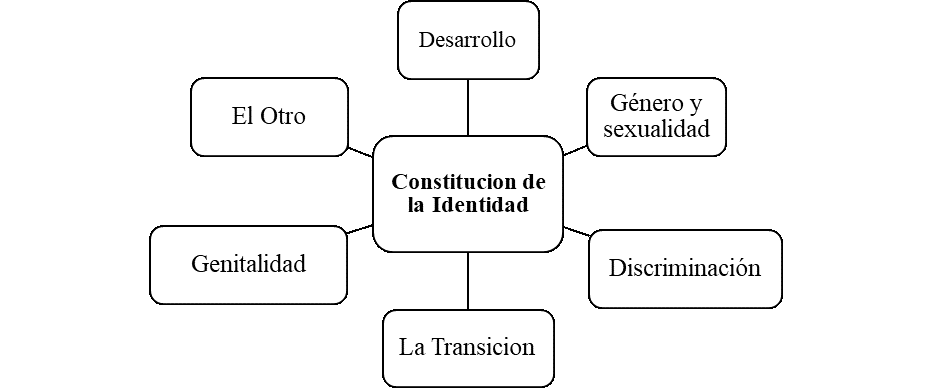
\includegraphics[width=0.75\textwidth]{categorias}
    \caption{Diagrama de categorías}\label{fig:categorias}
\end{figure}

A continuación realizaremos una descripción de cada una de ellas junto con los
verbatim que les dan origen.
Adicionalmente presentamos el razonamiento e interpretación que damos a cada
categoría y sus implicaciones caso a caso para el cumplimiento de los objetivos
de investigación.
El orden de presentación de las mismas fue elegido
según la frecuencia de manifestación en las entrevistas realizadas.

En la sección~\ref{sec:discusion}, realizamos una discusión y análisis punto a
punto de cada una de las categorías.

\section{Presentación de la información}

Como se puede ver resumido en la figura~\ref{fig:categorias}, hemos elaborado
seis (6) categorías. Dentro de estas categorías ‘La transición’ es uno de los
componentes identificados como constitutivo del proceso de construcción de la
identidad de las personas trans. Procederemos a explorar el contenido de cada
una de las categorías identificadas.

\subsection{Desarrollo}

Esta categoría se encuentra compuesta por elementos que
abarcan desde etapas tempranas de la niñez y del desarrollo. Elementos como la
relación del individuo con su escolaridad y compañeros de clases. También
elementos de la constitución de la identidad de género que se hacen presentes
dentro de la pubertad y los conflictos que estos puedan causar a los
participantes También incluye el papel que juega la familia dentro de la
constitución de la identidad, así como la forma de aproximarse a los problemas.
Todos estos son elementos que pueden marcar la construcción de identidad de una
persona.

\begin{figure}
    \centering
    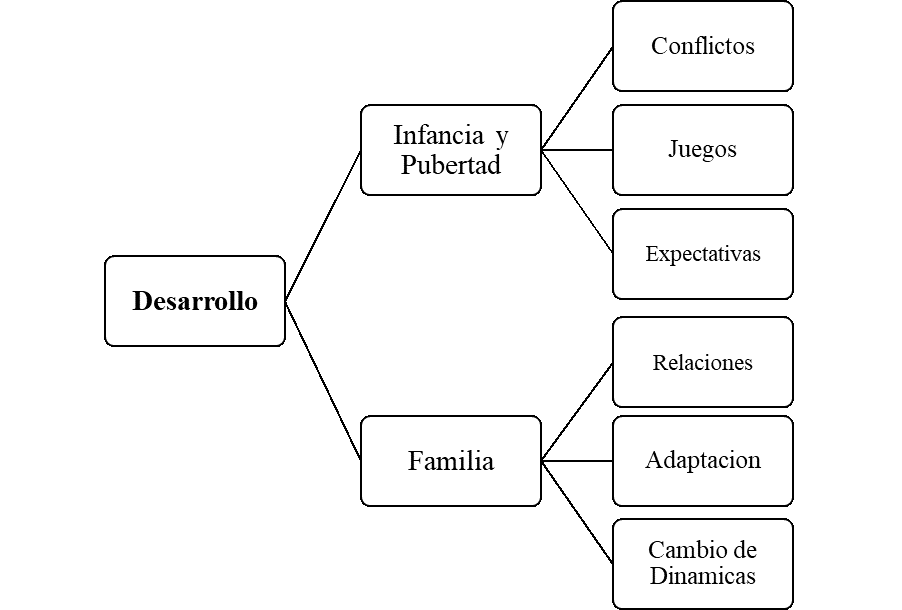
\includegraphics[width=0.75\textwidth]{desarrollo}
    \caption{Diagrama ‘desarrollo y familia’}\label{fig:desarrollo}
\end{figure}

En esta categoría confluyen elementos de conflicto, así como las experiencias que
permitieron el manejo de los mismos en los participantes y que
consecuentemente se transformaron en estrategias de afrontamiento. Se debe tomar
en cuenta que en esta categoría se presentan los distintos tipos de relación
establecidas tanto en niveles académicos como familiares entre la infancia y
pubertad de los participantes.

Existen dos subcategorías dentro de este factor. Una de ‘infancia y pubertad’,
que reporta sobre las experiencias de desarrollo y formativas en la juventud, y
otra de ‘familia’. Esta habla acerca de la influencia de los lazos y ambiente
familiar durante el desarrollo.

\subsubsection{Infancia y pubertad}
Dentro de esta subcategoría se pueden
encontrar elementos que parecen ser transversales a lo largo de la vida del
individuo. Al ser tanto la infancia como la pubertad etapas tempranas de
desarrollo y constitución se pudo identificar elementos que parecen sentar las
bases para la formación de otros elementos que le permiten al individuo constituirse
como persona. Entre estos elementos cabe resaltar la presencia de conflictos
como lo expresa el caso~1 (verbatim):

\begin{verbatim}
…bueno me identificaba como niño pero me gustaba todo las cosas
de niña. De hecho, siempre pedía al niño Jesús cosas de hembra, por ejemplo,
barbie, oso etcétera. Por su puesto, jamás me traía lo que pedía y era muy
triste para mí, una era inocente y el niño Jesús me dejaba una carta explicando
que eso eran cosas de niña y me traía patineta bicicleta carrito y a mí no me
gustaba…
\end{verbatim}

Este elemento puede estar ligado al rechazo que pueden vivir, según lo expresado
por el caso~1 (verbatim):

\begin{verbatim}
…en la escuela era algo terrible por el bullying, pero yo
siempre imponía carácter y jamás me deje amedrentar por nada ni nadie. De hecho
me agarre a golpes y me expulsaron por 10 días…
\end{verbatim}

O a tener su raíz en conflictos por la constitución de su identidad como lo
expresan con los siguientes verbatims.

Caso~1:

\begin{verbatim}
…yo lloraba porque no me entendía y me sentía mal.
\end{verbatim}

Caso~2:

\begin{verbatim}
  …me criticaban mucho como me vestía, pero es lo que me gusta.
\end{verbatim}

Y caso~3:

\begin{verbatim}
…siempre era el raro del grupo…
\end{verbatim}

La aparición de estos conflictos entra en contacto con las aproximaciones a los
roles de género que suceden por primera vez en la infancia por medio de los
juegos y que perduran a lo largo de la vida de un individuo, como se evidencia
en el relato del caso~1:

\begin{verbatim}
…a mí me decían que tenía que jugar con carritos y no con
muñecas porque eso es de niñas y yo no era una…
\end{verbatim}

Y del caso~3:

\begin{verbatim}
…me gustaba tener el cabello corto y no me arreglaba pero mis
padres me decían que tenía que arreglarme para poder verme linda…
\end{verbatim}

 Un elemento que se ve relacionado con la presencia del conflicto de identidad
 es que la aprehensión del mismo lleva al individuo a buscar o considerar el
 daño que puede causar el no lidiar con esta situación y es por eso que hay
 comentarios como el emitido por el caso~3 quien expresa sobre su
 adolescencia:

 \begin{verbatim}
Descubrí que tenía que hablar de esto con alguien o me iba a volver loco.
 \end{verbatim}

 Este verbatim, trae a la luz el malestar que nace en el individuo por este
 conflicto de identidad, posiblemente el hecho de estar en una situación de la
 cual se tiene poca o ninguna información al alcance del individuo hace que el
 malestar por el conflicto sea mayor y pueda tener consecuencias más peligrosas
 para la identidad de la vida del individuo.

\subsubsection{Familia}

Otro de los componentes de la categoría ‘Desarrollo’ es la subcategoría
denominada \emph{Familia}. Según lo expresado por los participantes existen obstáculos para la discusión intrafamiliar de la identidad, por ejemplo, el
caso~3:

\begin{verbatim}
…en mi casa siempre era un conflicto hablar sobre cómo me sentía.
\end{verbatim}

Caso~2:

\begin{verbatim}
Mi mamá me decía, ‘hija arréglate un poco’ ó ‘te verías muy linda
con vestido’ y yo le decía que no me gustaba eso y venía el regaño.
\end{verbatim}

Esta subcategoría influye en la constitución del individuo y modela su
desarrollo, en aspectos como la forma de establecer relaciones,
tomando lo expresado por el caso~2:

\begin{verbatim}
…la relación con mis padres es distinta, a mi madre le costó más
aceptarme. A mi padre, después de explicarle, lo entendió con más facilidad,
incluso suelo pasar por su trabajo, es moto taxista.
\end{verbatim}

Un elemento que resaltan los participantes es el cambio de dinámicas dentro de
la familia que se da producto de asumirse como persona transgénero. Como se observa en
el relato del caso~1:

\begin{verbatim}
…mi madre al principio le costó mucho aceptarlo y mi papá le
dijo a mis hermano que por qué no me quedaba como yo. Era que él me aceptaba gay
más no vestido de mujer y jamás me permitió aclararle los conceptos que tenía
errado y hasta hoy no me trata ni mi padre ni mi hermano menor…
\end{verbatim}

Estos verbatims asoman que dentro de las familias de los individuos transgéneros
existe una innegable presencia de conflicto generado por la nueva identidad
asumida por el mismo. El cómo esta identidad interactúa con las prenociones de
la familia suma a la conflictividad durante el desarrollo. Es posible que esta
situación esté relacionada con el propio conflicto interno que pueden vivir
personas transgénero como consecuencia de la falta de acceso a información que
permita aclarar sus dudas.

Esto podría ser un indicador de las percepciones hegemónicas sobre la sexualidad
y como estas moldean las diversas interacciones entre los individuos. Se
observa en el verbatim del caso~1 que por parte de su padre existe aún una
confusión entre lo que es la orientación (los gustos del individuo) y su
identidad (como el individuo se observa a sí mismo) sexual.

\subsection{Género y sexualidad}

La siguiente categoría que permite la constitución de identidad en los
participantes es la de \emph{género y sexualidad}. En esta categoría se
presentan elementos como la constitución de la identidad que tienen su raíz en
etapas tempranas de la vida. Con base a lo expresado por los participantes se
generaron las siguientes subcategorías: Identidad de género, Socialización de género
y Orientación Sexual.

En la figura~\ref{fig:genero} se pueden observar los elementos constitutivos de
la categoría.

\begin{figure}
    \centering
    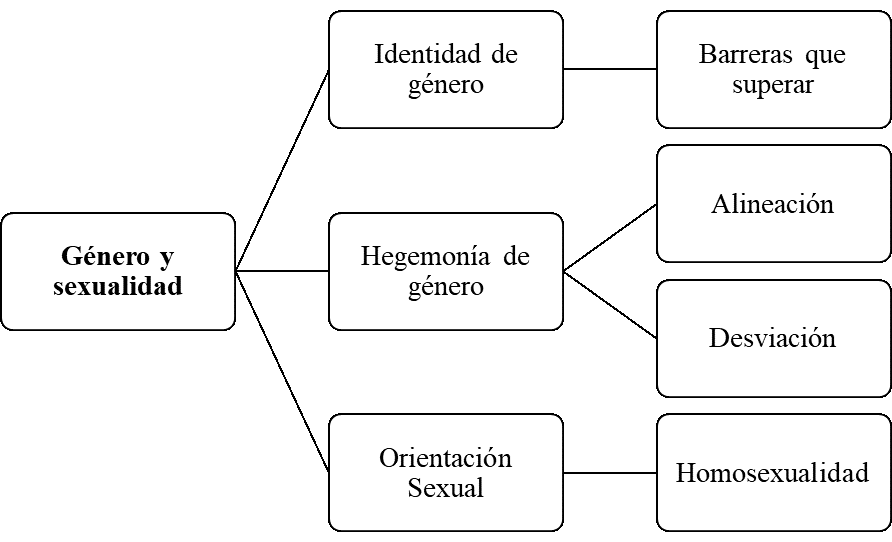
\includegraphics[width=0.75\textwidth]{genero}
    \caption{Diagrama ‘género y sexualidad’}\label{fig:genero}
\end{figure}

\subsubsection{Identidad de género}

Esta subcategoría se mostró como la más importante dentro de lo expresado por
los participantes principalmente porque ha sido el componente central con
el que se enfrentaron en la constitución de su identidad. Esto se puede ver
reflejado en lo expresado por el caso~2:

\begin{verbatim}
…el momento más feliz de mi infancia es cuando me pude vestir
de Ángel Gabriel en un nacimiento viviente que hicieron en mi escuela. Mi mamá
no quería pero yo me sentía en las nubes porque por un momentito pude verme como
quería.
\end{verbatim}

Este conflicto de identidad también se hace visible dentro del relato del caso~3
cuando expresa:

\begin{verbatim}
…no es que solo me gustaba vestirme como hombre, es que pensaba
como uno también.
\end{verbatim}

Esto también lleva a cuestionarse el papel de los roles de género en la
concepción de este ‘pensar como’ y pone en perspectiva crítica el significado de
‘pensar como hombre’ o ‘pensar como mujer’. Dentro del relato del caso~1
comenta:

\begin{verbatim}
Cuando era pequeña no me molestaba, pero cuando empecé a
desarrollarme le rezaba a Dios para que por favor me salieran senos.
\end{verbatim}

Estos verbatims permiten identificar algunos aspectos relacionados con el
conflicto de identidad de los individuos. Elementos como el verbatim expresado
por el caso~2 que considera un recuerdo muy feliz el poder mostrar una
expresión de género acorde a la identidad que, ya para esa etapa de su
desarrollo, sentía era la de él. Además, esto se puede reforzar con el verbatim
del caso~1 cuando expresa que le causaba preocupación y ansiedad el hecho que
sus senos no se desarrollaran junto con el resto de su cuerpo.

Además, se presenta la dicotomía entre lo que las personas sienten que son, las
expectativas de como esperan verse y la imposición de la identidad que se
les asignó por haber nacido con un sexo específico.

\subsubsection{Socialización de género}

Esta subcategoría surge de la relación que los participantes han tenido con
elementos propios de los roles de género, especialmente del rol del género
asignado según su sexo biológico. Es decir, está compuesta por aquellos
elementos que demarcan la diferencia entre lo femenino y lo masculino. Elementos
dentro del relato del caso~1 hacen presentes estas diferencias:

\begin{verbatim}
…el niño Jesús me dejaba una carta explicando que eso eran cosas de niña y me
traía patineta, bicicleta, carritos y a mí no me gustaba…
\end{verbatim}

Así como lo expresado por el caso~3:

\begin{verbatim}
Me decían que tenía que sentarme bien y como niña, y yo me preguntaba ¿cómo es
eso?
\end{verbatim}

Partiendo de estos verbatims se puede observar que existe un modelaje hacia el
individuo sobre el conjunto de expectativas específicas relacionadas con cada
género. Además, se evidencia la insistencia de parte del entorno social por
conformarse a aquellas expresiones de género propios del género que les fue
asignado por su sexo biológico en el momento del nacimiento.

En estos verbatims se pueden observar, además, que existe una atribución, bien
sea masculina o femenina, sobre cosas (juguetes), o actos comportamentales.
Estas atribuciones son arbitrarias, pues en el caso del verbatim del caso~1,
los juguetes que le regalaban podían también ser asociados como juguetes de
niños o en el caso del caso~3, que condiciones específicas son las que
determinan el cómo se debe sentar una persona dependiendo de su sexo o género.
Esto forma parte de los roles y expresiones de género, y son los primeros
elementos a los que los participantes parecen demostrar rechazo.

\subsubsection{Orientación sexual}

El último componente de la categoría de Género y sexualidad es la subcategoría
de ‘Orientación Sexual’. En esta subcategoría se presentan aquellas inquietudes
e incongruencias que surgieron en la vida de los individuos al momento de buscar
pareja sexual y romántica. No solo fundamentado en aspectos físicos sino también
emocionales. El caso~3 relata:

\begin{verbatim}
 Yo solía tener sexo telefónico con una amiga en bachillerato y en una de esas
 fantasías yo era un hombre y ella lo seguía y esas cosas sucedían y el primer
 nombre de mi personaje fue Alex y ahí empezó a asomarse algo que se transformó
 en lo que soy ahora.
\end{verbatim}

Este verbatim asoma un elemento resaltante de la orientación sexual en personas
transgénero, su consolidación se hace presente durante la adolescencia,
permitiendo de esta manera influir en la constitución identitaria del individuo.
Esto parece ser un elemento compartido en común tanto entre personas cisgénero
como transgéneros.

Así se puede interpretar que las personas transgénero dan muestras de su
identidad de género en los juegos sexuales de exploración
tempranos. Reforzando la idea de que estos presentan preferencia por presentarse
según su género sentido desde muy temprano en su vida.

Existe, además, una confusión asociada a la expresión de la sexualidad cuando no
se tienen interiorizados los conceptos propios de lo transexual o transgénero.
El caso~3 afirma al referirse sobre su experiencia sexual temprana:

\begin{verbatim}
Al principio todo hombre trans se cree lesbiana.
\end{verbatim}

El caso~2 refuerza esta confusión:

\begin{verbatim}
…yo no conocía de lo trans ni nada, pensaba que era homosexual y ya…
\end{verbatim}

Esto refuerza la concepción de que la orientación puede ser confundida con la
identidad, sobre todo cuando no existe un concepto claro de la transexualidad o
transgenerismo en la persona.

\subsection{Discriminación}

Esta categoría representa el segundo elemento más importante según lo expresado
por los participantes. La discriminación parece encontrarse inevitablemente
ligada a la condición trans. Los eventos discriminantes a los que ellos se ven
sujetos abarcan desde situaciones de rechazo como los presentes en las vivencias del caso~1:

\begin{verbatim}
La población trans está muy expuesta al rechazo, porque no nos entienden,
piensan que somos unos bichos raros y nos ven y tratan como tales.
\end{verbatim}

Estas situaciones pueden llegar a convertirse en actos de acoso o bullying como
los que comenta haber vivido el caso~2:

\begin{verbatim}
Cuando inicié mi transición los compañeros de trabajo de mi papá se metían
conmigo, hasta que un día les ofrecí unos golpes y todo cambió.
\end{verbatim}

 Puede incluso llegar a generar en el individuo miedo, así como una sensación de
 inseguridad como lo expresa el caso~3:

 \begin{verbatim}
Estando en Ecuador supe de un trans al que violaron y mataron y la verdad me dio
miedo.
 \end{verbatim}

Con base a estos verbatims se puede establecer un punto de referencia que
permite generar subcategorías en lo que se puede considerar una categoría
principal denominada \emph{Discriminación}. Los componentes de esta categoría se
pueden observar en la figura~\ref{fig:discriminacion}. Así mismo partiendo de
estos verbatims se puede pensar que las experiencias discriminantes son
trasversales a la vida de una persona transgénero ya que se pueden presenciar
tanto en etapas tempranas como en etapas más adultas de la vida de los
participantes como se presenta a continuación.

\begin{figure}
    \centering
    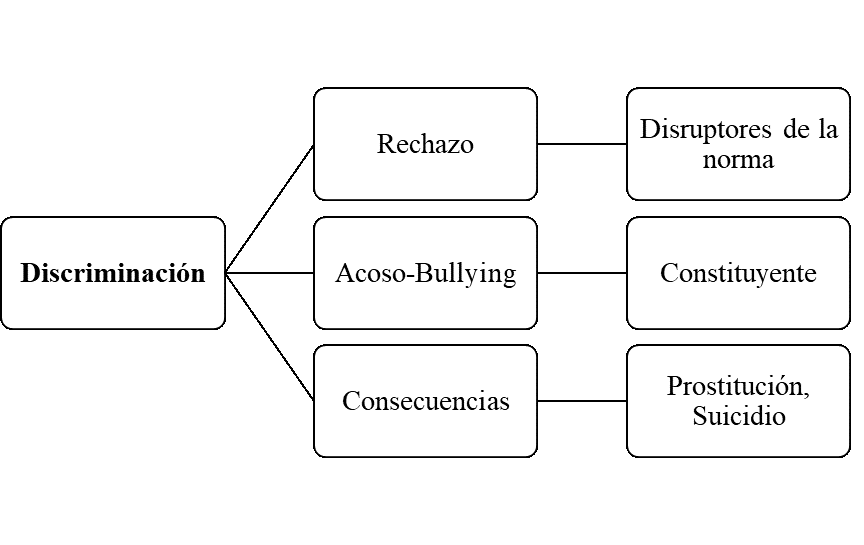
\includegraphics[width=0.75\textwidth]{discriminacion}
    \caption{Diagrama ‘discriminación’}\label{fig:discriminacion}
\end{figure}

\subsubsection{Rechazo}

Un elemento común en el discurso de los participantes es la presencia de
vivencias de rechazo, es decir situaciones en las que han sido víctimas de actos
que impiden su participación regular como miembro de la sociedad y que pueden
atentar contra la integridad de un individuo. Esto se hace evidente dentro del
relato del caso~2 cuando expresa:

\begin{verbatim}
Yo solía ir a comprar ropa de hombre y las vendedoras me decían que no. Por qué
compraba eso si yo era mujer y me miraban como con asco y yo les respondía que
lo hacía porque me gusta la ropa y porque tengo la plata para hacerlo.
\end{verbatim}

Así como también dentro del relato del caso~1 cuando comenta que:

\begin{verbatim}
…era horrible cuando me tocaba sacarme la cédula y me obligaban a ir vestida
como hombre, el personal que me atendía se ponía muy hostil conmigo cuando
llegaba maquillada.
\end{verbatim}

Estos verbatims permiten visibilizar elementos discriminantes que afectan la
expresión de identidad de género de los individuos transgénero. El rechazo que
pueden vivir parece tener sus raíces en condiciones socialmente construidas
relacionadas con lo que se espera que sea la expresión de género de una persona
de sexo masculino o femenino. Esta identidad que se le impone a las personas
transgéneros (sin importar su etapa de transición) afecta el proceso
que transitan, generando malestar en el individuo. Debido a su decision de
alinear su expresión de género con la identidad de género con la cual se sienten
identificados se ven criticados y despreciados por comentarios como los
expresados por los participantes.

\subsubsection{Acoso / Bullying}

Otro elemento importante dentro de la vivencia de la discriminación por parte de
los participantes es la relación que ellos desarrollan con el acoso o el bullying.
El caso~1 expresa que:

\begin{verbatim}
…en la escuela era algo terrible por el bullying, pero yo siempre imponía
carácter y jamás me deje amedrentar por nada ni nadie. De hecho, me agarre a
golpes y me expulsaron por 10 días…
\end{verbatim}

Esto demuestra que desde etapas tempranas de su vida se encuentran presentes
elementos de acoso. El caso~2 expresa en su relato también que las situaciones
de acoso se pueden vivir en ambientes académicos:

\begin{verbatim}
Mientras estudiaba para sacar mi título de sexólogo me pasó que una docente era
particularmente agresiva conmigo, porque una vez le respondí feo. La razón de
esto fue porque ella estaba cuestionando mi identidad. Pero nada al final le
saqué un 20 y le callé la boca.
\end{verbatim}

Resalta el hecho de que, por su condición como personas transgénero, hechos como
el acoso o el bullying se hagan presentes con gran peso dentro del relato de los
participantes. Es también importante evaluar las estrategias con las cuales los
participantes lidian con estas situaciones. Parece ser que dependiendo del tipo
de acto que vaya en contra de ellos, ya sea violencia física o simbólica, para
poder ser redimido o valorado positivamente es necesario rebasar o exceder
aquellas expectativas que han sido impuestas por el agresor hacia el agredido.
Esto podría acarrear consecuencias negativas para la persona transgénero pues
vivir con la constante presión de tener que ser valorado solo por sus logros
puede llegar a ser una fuente de estrés negativo en la vida de la persona
transgénero.

\subsubsection{Consecuencias}

Por último, es necesario remarcar que tanto el rechazo como el acoso o bullying
tienen consecuencias en la vida de la persona transgénero. Por ejemplo, el caso~2
relata:

\begin{verbatim}
Hace poco supe de un caso de una chica trans, ella aún no comenzaba con su
tratamiento hormonal pero ya estaba expresando una identidad de género con la
que se sentía cómoda. La cosa es que por ser trans su familia la botó de la casa
y terminó en situación de calle, prostituyéndose para sobrevivir hasta que la
mataron hace una semana, la encontraron en un monte.
\end{verbatim}

Además, se puede tomar en cuenta el comentario del caso~1, quien labora en una
oficina de atención social:

\begin{verbatim}
…aquí nos llegan muchos casos de personas trans que se quedan sin casa o trabajo
por querer ser felices, principalmente pasa con chicas, algunas se terminan
suicidando…
\end{verbatim}

 Esto pone sobre la mesa las consecuencias negativas que tienen situaciones
 aversivas producto de la discriminación. Estas siempre son una sombra de temor
 sobre la vida de las personas trans y es lo que les pone en riesgo de
 situaciones como la prostitución o el suicidio. Estas consecuencias tienen su
 origen en los elementos anteriormente mencionados en las subcategorías previas.
 Tanto vivir el rechazo por parte de otras personas, así como el acoso y la
 necesidad de tener que encontrar estrategias de supervivencia que permitan al
 individuo valorarse ante otros como par hace que la vida de las personas
 transgénero este cargada de dificultades.

\subsection{La Transición}

En esta categoría agrupamos los elementos relacionados con el tránsito entre un
género o sexo a otro. Usualmente del género o sexo asignado al nacer hacia el
género o sexo deseado. Los elementos componentes de esta categoría se pueden
apreciar en la figura~\ref{fig:transicion}. Estos incluyen la elaboración que
realizan los participantes del proceso de transición en sí mismo desde su
subjetividad, la apariencia física y el conocimiento sobre los procedimientos
médicos, quirúrgicos y sociales que permiten llevar a cabo la transición.

\begin{figure}
    \centering
    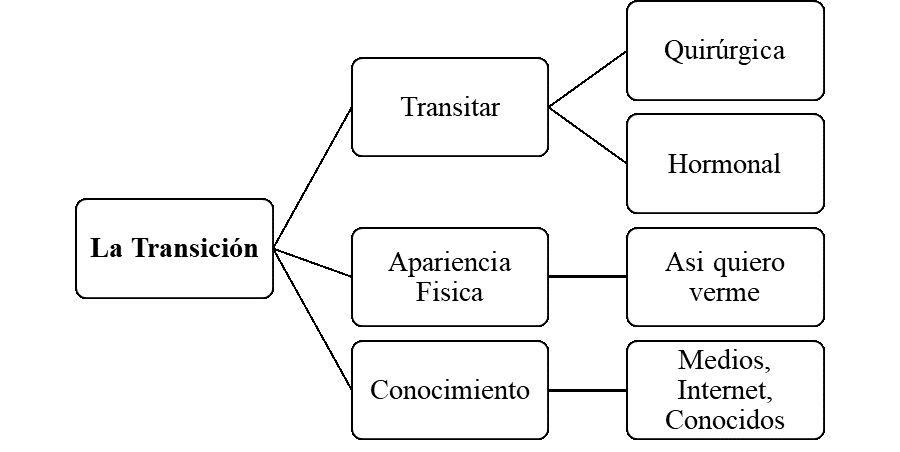
\includegraphics[width=0.75\textwidth]{transicion}
    \caption{Diagrama ‘la transición’}\label{fig:transicion}
\end{figure}

\subsubsection{Transitar}

Según lo expresado por los participantes, el transitar va más allá de ser un
simple hecho, también es una herramienta. La transición es un medio que
les permite llega a ser quien ellos sienten que realmente son. El transitar
puede abarcar aspectos quirúrgicos y/u hormonales, y como lo expresa el caso~2:

\begin{verbatim}
…las hormonas ayudan pero la operación libera…
\end{verbatim}

El caso~3 coincide al comentar:

\begin{verbatim}
…las hormonas ayudan, cuando dejé de tomarlas perdí todo, era una niña…
\end{verbatim}

Estos comentarios evidencian que existe una valoración de la alteración
quirúrgica como más importante que el tratamiento hormonal. Además, se considera
la transición quirúrgica como un objetivo final o como una acción liberadora.
Cabe preguntarse lo que sucedería si no se puede concretar una transición
quirúrgica.

Sin embargo, lo dicho por el caso~3 hace referencia a como el componente
hormonal tiene una importancia por su cualidad inmediata. Debido a que permite
una visibilización a corto plazo de la identidad, más explícita que una
operación. Los efectos de la transición hormonal son visibles mientras que la
cirugía genital no lo es. De igual manera, el tratamiento de reemplazo hormonal
requiere de una toma constante. Por ello dejar de tomarlo implica una reversión
rápida de sus efectos.

Por otro lado, se tiene que tomar en cuenta lo expresado por el caso~1:

\begin{verbatim}
…por cuanto mi apariencia física y genética me han ayudado en la transición lo
cual ha sido muy fácil, de hecho, no he tomado hormona nunca…
\end{verbatim}

Esto permite indicar que la importancia no está colocada en la toma de hormonas
en sí misma. Sino que la importancia está en los cambios de aspecto físico y de
visibilidad que se producen como resultado de la influencia hormonal. En esta
instancia el caso~1 indica no necesitar de la toma hormonal pues su aspecto ya
es femenino en sí, lo que es su objetivo último.

Este elemento se relaciona con la Apariencia física, pues es el aspecto—
efectivamente la expresión de género—lo que la persona transgénero desea alterar. La
función biológica es secundaria a sus efectos sobre la expresión.

\subsubsection{Apariencia física}

Aquí podemos encontrar la expresión de la relación sexo-género. Es decir, la
relación existente entre el género y las caracterísitcas sexuales secundarias.
Se debe tomar en cuenta que dentro de esta relación hay particularidades que
tienen un mayor peso o que suelen tomarse más en cuenta para su expresión como
lo plantea, por ejemplo, el caso~3 al referirse a un tiempo en el cual dejo de
tomar hormonas:

\begin{verbatim}
  …perdí el torso perdí básicamente eso, la libido cambio…
\end{verbatim}

Esto implica que el poder verse y expresarse en concordancia con los rasgos del
sexo o género al que se transita es fundamental. Además de que también tiene
importancia el cómo se siente. Aquí refleja uno de los efectos de la
testosterona sobre el impulso o deseo sexual. No sólo desea verse, sino sentir
su propio cuerpo como aquel del sexo deseado.

Además de esto se puede tomar en cuenta lo expresado por el caso~2:

\begin{verbatim}
…le tengo terror a la regla porque soy hombre y a los hombres no les debe venir
eso.
\end{verbatim}

Este refleja la importancia del ‘sentirse como’. No se trata, sin embargo, de
una búsqueda funcional. La menstruación como fenómeno biológico tiene un
objetivo reproductivo. No es la función o la menstruación lo que rechaza el
participante sino el desarreglo con la conformación estereotípica de la
dicotomía sexual. No se rechaza el tener la menstruación sino el hecho de tener
la menstruación siendo hombre. Esto no se ajusta con la construcción física
propia del hombre y por ello es rechazado.

Este elemento visibiliza la concepción de concordancia de sexo/género que
prevalece, pues estar alineado no solo puede significar tener características
propias de un sexo o género, sino que también puede significar no tener o evitar
las asociadas con otro.

\subsubsection{Conocimiento}

La subcategoría de conocimiento hace referencia tanto a cómo los participantes
reafirmaron o conocieron su condición, así como a la manera con la cual entraron
en contacto con el proceso que les permitiese su transición. En esta
subcategoría resalta el papel de los medios para visibilizar la
condición trans, el caso~2 expresa que:

\begin{verbatim}
…yo no conocía de lo trans ni nada, pensaba que era homosexual y ya, pero
luego un día viendo televisión con mi novia de ese momento pasaron el primer
capítulo del programa ‘Taboo’, por NatGeo y ahí presentaron a una persona trans
y mi novia me dijo, mira ella dice que se sentía como tú dices que te sientes
y pues eso me dejó pensando.
\end{verbatim}

Podemos entonces afirmar que hay aún un desconocimiento de la diferencia entre
la orientación sexual y la identidad sexual. Además, se evidencia que es
necesario para las personas trans aprender e interiorizar los significados de:
género, sexo, identidad sexual y transición, para poder dar sentido a la propia
experiencia. Sin estos significados no es posible para la persona trans comenzar
a poner en cuestionamiento el género asignado y la propia identidad.

Por otro lado, se puede tomar como referente la experiencia del caso~1 que
expresa:

\begin{verbatim}
Me di cuenta y logré comprender que era ser trans a los 40 años de edad, porque
desconocía que era ser trans, de hecho, en mi ignorancia tampoco sentía que me
identificaba como gay porque me sentía mujer pensaba como mujer y eso no lo
entendía, todo eso lo viví en silencio por 40 años jamás dije nada por el
rechazo que pudiera sentir hasta que me hablaron de personas trans y fue allí
cuando comencé a entender que yo era una mujer transexual.
\end{verbatim}

Esto refuerza la diferencia entre la orientación, la identidad sexual y la
identidad de género. También señala la vivencia privada y subjetiva de la
mayoría de las personas transgénero quienes suelen mantener su confusión en
silencio por miedo al rechazo. Refuerza también la importancia de la
comunicación de los conceptos alrededor del género y la identidad para poder
asumirse a sí mismo como persona trans.

El caso~1 añade:

\begin{verbatim}
Lo descubrí a los 40 años gracias a mi psicólogo que me realizo una terapia y
allí fui abriéndome y diciendo lo que sentía y fue cuando supe que era una mujer
trans.
\end{verbatim}

Esto potencia el rol del psicólogo como voz autorizada y mediador en el proceso
de transición, calmando el malestar del individuo. El psicólogo aquí también
ejerce la función de educador de la persona con un malestar que no ha podido
significar o expresar de una manera satisfactoria. La adquisición de conceptos
psicológicos y los símbolos propios de la identidad de género le permite a la
persona trans construir su propia interpretación de su condición e identidad.

\subsection{Cuerpo y genitalidad}

Esta categoría se centra en el aspecto biológico de la identidad del individuo
pero no abarca componentes hormonales o cromosómicos como tales sino que se
centra únicamente en el aspecto fenotípico genital desde lo estético y lo
sensitivo así como lo que representa para los participantes este aspecto de su
cuerpo.

En la figura~\ref{fig:genitalidad} se pueden observar los componentes de esta
categoría.

\begin{figure}
    \centering
    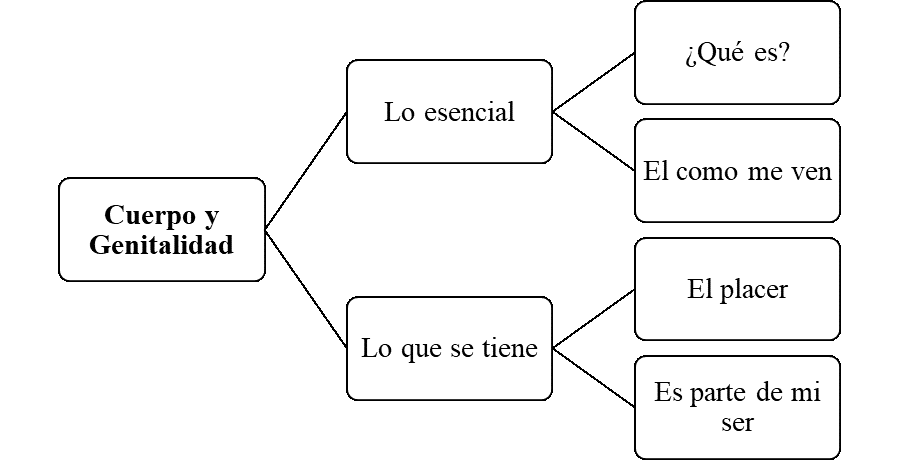
\includegraphics[width=0.75\textwidth]{genitalidad}
    \caption{Diagrama ‘cuerpo y genitalidad’}\label{fig:genitalidad}
\end{figure}

\subsubsection{Lo esencial}

Esta subcategoría abarca aquello que los participantes consideraron de mayor
importancia sobre su relación con el cuerpo, es interesante observar que el
componente genital no tiene una primacía en la construcción de su identidad. Si
se toma en cuenta lo expresado por el caso~1 cuando se le pregunta por la
transición quirúrgica:

\begin{verbatim}
Solo me decidí operar el pecho y ponerme mamas.
\end{verbatim}

Esto es resaltante porque, aunque el sentirse como perteneciente al género
deseado es importante, aún más importante es ser recibido y aceptado socialmente
como el género con el cual se identifica. Esto permite la validación social de la identidad del individuo. En este sentido la opción quirúrgica
es evaluada en su función para la expresión del género deseado, y por ello se le
da prioridad a la mamoplastia.

También el caso~3 comenta:

\begin{verbatim}
¿Para qué un trans se opera el pecho? para poder quitarse la camisa.
\end{verbatim}

Y el caso~2 agrega:

\begin{verbatim}
Quiero poder operarme para poder quitarme la camisa y hacer cosas normales.
\end{verbatim}

Una vez más se ve reforzado que el cambio corporal esencial es aquel que permite
la inserción social. Parece resaltar la importancia de lo que se considera
caracteres sexuales secundarios sobre los primarios. Es decir, es más importante
lo que ve el otro en público que lo que se ve en privado. Comentarios como el
del caso~2:

\begin{verbatim}
…a mí me encanta ir al gimnasio y tener la espalda ancha, me
siento como un monstruo.
\end{verbatim}

Refuerzan la idea de que lo esencial es mostrarse para todos y ser recibido cómo
el género con el cual hay identificación. Aquí el uso de monstruo es un sentido
positivo. Desde la mirada que asocia a un ‘monstruo’ con fuerza, tamaño físico,
poder y vitalidad. Características estereotípicamente asociadas con la
masculinidad. Además de que la idea que yace detrás es la realización de las
interacciones sociales típicas del rol de género por el que se desea pasar. En
este caso, el hombre que va al gimnasio es para hacerse fuerte, muscular, grande
y poderoso.

\subsubsection{Lo que se tiene}

Además de lo encontrado en la subcategoría anterior los participantes expresaron
que es más importante el genital que se tiene, y como este permite relacionarse
con una pareja, que buscar que los genitales coincidan con el género con el que
se identifican. Es por esto que la presente subcategoría nace, tomando en cuenta
comentarios realizados por los participantes, como por ejemplo, lo expresado por
el caso~3:

\begin{verbatim}
Lo mío es mío y con esto resuelvo.
\end{verbatim}

A lo que le agrega:

 \begin{verbatim}
…un pene falso a nivel sexual es solo un instrumento.
 \end{verbatim}

También comenta el caso~2 sobre la cirugía de reasignación de sexo:

\begin{verbatim}
Eso después hace que pierdas sensibilidad
\end{verbatim}

Se puede interpretar de estas expresiones que existe una preferencia a acercarse
a la relación sexual desde los genitales con los que se nació. La genitalidad
propia del género con el cual se sienten identificados es un aspecto secundario.
A esto se le puede sumar la importancia asignada a la cirugía de mamas, ya sea
para removerlas o crearlas. Esto está relacionado al valor exclusivamente
femenino que tienen los senos en la sociedad como un aspecto visual y evidente
que señaliza la femineidad.

\subsection{El Otro}

Esta categoría fue nombrada debido al peso que tiene la presencia del otro en
la vida de cada individuo dentro de la sociedad. Debido a que el ser humano es
un ser intrínsecamente social existen principios que rigen las interacciones, así
como diversas formas para poder satisfacer las necesidades que surgen de estas
interacciones. Tomando en cuenta que la condición trans puede ser disruptiva
dentro de lo socialmente aceptado se puede comprender que la importancia del
otro cobra un sentido particularmente fuerte en estos casos pues el otro puede
moldear la forma en la que se asume el género, así como patrones de
comportamientos, vestimenta y roles que permitan al individuo expresarse según
el género con el que se sienten identificados.

En la figura~\ref{fig:otro} se puede observar la estructura de los elementos que
componen esta categoría.

\begin{figure}
    \centering
    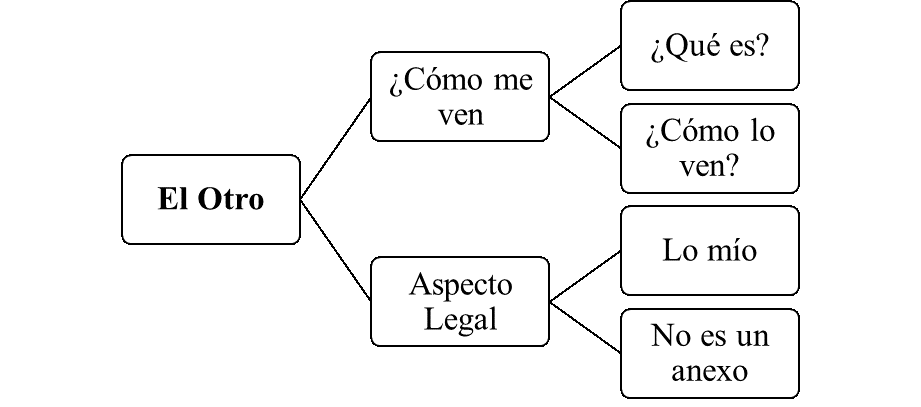
\includegraphics[width=0.75\textwidth]{otro}
    \caption{Diagrama ‘el otro’}\label{fig:otro}
\end{figure}

\subsubsection{Cómo me ven}

La primera subcategoría es sobre la percepción general que tienen los demás de
la persona transexual, o al menos cómo estos la conciben. Tomando en cuenta lo
expresado por el caso~3:

\begin{verbatim}
  …me solían ver como el raro…
\end{verbatim}

Caso~1:

\begin{verbatim}
Les causa impresión y cambia todo cuando doy mi cedula para pagar maquillaje.
\end{verbatim}

Parece ser que el rol transgresor de la condición transgénero es lo que permea
el trato que estas personas reciben. Es decir, cuando alguien interactúa con una
persona trans el saber o no que se encuentra hablando con una persona trans va a
afectar el trato que reciban. Además, el trato que reciben es percibido como
regular hasta que la otra persona se da cuenta que está interactuando con
alguien trans,

El caso~2 agrega:

\begin{verbatim}
La gente juzga mucho y como que esperan más de ti, que seas más hombre que otro
hombre o más mujer que otra mujer.
\end{verbatim}

Esto demuestra como la persona transgénero se ajusta a la mirada de los otros
por medio de asumir expresiones propias del género con el que se encuentran
identificados. Bien sea mediante comportamientos o alterando su apariencia
física. Resalta el calificativo utilizado por el caso~2 ‘más hombre que otro
hombre o más mujer que otra mujer’. Esto implica que existe una presión y una
expectativa por cumplir con los estereotipos de los roles de género. Incluso más
allá de lo que sería razonable para una persona cisgénero.

Cabe señalar en este aspecto un comentario realizado por el caso~3:

\begin{verbatim}
Yo llevo un aparatico para poder usar el baño de hombres, porque sabes los
hombres se miran a veces y a mí me gusta usar un urinario y orinar de pie.
\end{verbatim}

Este relato entra en contacto con lo expresado por el caso~1:

\begin{verbatim}
Yo soy muy coqueta, me hice así una vez me asumí mujer trans, antes no me
arreglaba mucho.
\end{verbatim}

Parece ser que el adaptar o incluir roles de conducta propios de un género no es
un hecho exclusivo para la aceptación privada, sino es también un elemento
de validación con el otro.

\subsubsection{Aspecto legal}

Complementando a la subcategoría anterior se presenta el ‘Aspecto legal’, que
indica la forma en la cual son reconocidos legalmente las personas transgénero.
Este es un elemento constitutivo de su identidad debido a que al ser ciudadanos
de la República Bolivariana de Venezuela necesitan contar con la seguridad legal
de que sus derechos van a ser respetados y el primer paso es poseer una
identidad legal, como el caso~1 lo expresa:

\begin{verbatim}
…otro momento en el que fui muy feliz fue cuando pude sacarme la foto de la
cédula con maquillaje y expresándome como soy de verdad.
\end{verbatim}

El poder ser identificada legalmente según su expresión de género es algo muy
significativo pues los reafirma como ciudadanos con derechos. Si bien el cambio
de sexo en la identidad no es posible aún, ser reconocido en la fotografía de su
identidad y aparecer cómo realmente se expresan en el día a día representa una
pequeña victoria. El caso~2 refuerza este planteamiento comentando que:

\begin{verbatim} …cuando legalmente se nos pueda identificar sin ningún problema
pero va a ser una victoria muy importante, el siguiente paso sería quitarnos el
prefijo trans, yo soy un hombre y ya no un hombre trans, eso no es inclusivo.
\end{verbatim}

\section{Discusión}\label{sec:discusion}

Desde su concepción, la presente investigación ha tenido como principal foco de
interés proveer una mirada no patologicista a lo que es el transgenerismo, esta
propuesta nace de la necesidad de romper con la noción del transgenerismo como
una enfermedad mental—forma como ha sido catalogada desde aproximadamente la
década de los ochenta según manuales de diagnóstico como el DSM-IV y el CIE-10.
La visión del transgenerismo como un hecho antinatural o que no es normal viene
asociada a la construcción de identidades en la sociedad por medio de dicotomías
rígidas que facilitan la patologización de expresiones humanas que se salgan de
lo \emph{establecido}.

Esto entra en contraste con respecto a lo planteado por la Teoría Queer, que
como lo explican Fonseca y Quintero (2009) asume a la expresión de género como
un continuo; y que  si bien pueden existir extremos no son más que puntos de
referencia, marcadores, entre los cuales se pueden encontrar las diversas
expresiones de género y sexualidad del ser humano. Al tomar esto en cuenta
parece ser posible complejizar la condición transgénero y verla como un hecho
que sufre al ser simplificada por una visión dicotómica de la identidad sexual y
la identidad de género.

Partiendo de la codificación realizada proponemos que la identidad de los
participantes se construye de una manera específica, marcada por las
interacciones que se llevan a cabo en su cotidianidad, desde su infancia hasta
su adultez. Es por esto que se presenta a continuación una discusión detallada
de las categorías elaboradas en base a lo recopilado en las entrevistas
realizadas a los participantes.

\subsection{Desarrollo}

Esta categoría nace de las vivencias de los sujetos desde su infancia, las
cuales se convierten en los cimientos que modelan la forma en la que se
desenvolverán en la sociedad. Es necesario remarcar que la condición transgénero
en los participantes es asumida no como una elección, sino como algo que es, no
es un capricho o moda, es un sentir real y auténtico que en muchos casos los
lleva a un estado de conflicto pues no se logra encontrar una forma de balancear
la identidad sentida y lo socialmente esperado.

Este conflicto se puede tomar como punto de partida para entender la identidad
transgénero. Algunos autores como Hernández, Rodríguez y
García-Valdecasas (2010), afirman que el malestar o conflicto que pueden sufrir
las personas transgéneros viene asociado a la dificultad que encuentran al tener
que identificarse o alinearse con modelos socialmente construidos sobre lo que
significa ser un hombre o una mujer. Esta visión parece también estar influida
por una perspectiva biomédica, asumiendo que el componente genital es el único
indicador determinante al momento de asumir una identidad de género, ya sea
masculina o femenina. Como muestra de esto se puede tomar en cuenta la
prevalencia de instrumentos de diagnóstico como el Manual diagnóstico y
estadístico de los trastornos mentales para identificar y clasificar a
una persona como transgénero y que relegan otros elementos propios de la
identidad humana como lo son elementos sociales, culturales,
históricos-personales que pueden influir en la constitución de la identidad del
individuo. Sin embargo, es necesario resaltar que la edición actual del DSM
(en este momento la quinta) ha ajustado su enfoque al fenómeno transgénero y ha
cambiado la nomenclatura por la cual se identificaba a esta condición.

Entonces esto lleva a cuestionar cual es la comprensión que se tiene sobre el
sexo, sexualidad e identidad desde una visión no científica y patologizadora.
Podría plantearse entonces que debido a una predominancia del discurso médico
esta visión se ve sesgada, limitando estos aspectos de la vida humana a aquello
que ha sido validado por una visión biomédica. Esta visión puede que sea la
que se reproduce en distintos núcleos familiares y que se cristaliza en los
miembros de la familia y que puede llegar a causar conflictos cuando uno de
estos miembros interactúa con, por ejemplo, la identidad transgénero.

En las entrevistas realizadas a los participantes se presentó un elemento en
común y es que tanto la infancia como la adolescencia fueron etapas críticas de
su desarrollo en las cuales entraron en contacto con su identidad como persona
transgénero. En estas etapas es cuando que surge la duda en ellos sobre la
incongruencia entre el género con el cual se identifican y las expresiones
(juegos, ropa, roles) que se les pedía, o se esperaba, que expresaran. A raíz de
este conflicto presentaban situaciones que afectan la dinámica familiar de los
participantes. Al existir una visión ligada a la relación que debe existir
entre un determinado sexo biológico y su expresión de género por parte de
miembros de la familia al entrar en contacto con la identidad transgénero de los
participantes podía llegar a causar confusión, así como conflictos.

Esto refuerza planteado anteriormente y es que la visión de lo que
significa ser hombre o mujer encuentra sus cimientos en estas etapas de la vida
de un individuo. Es en estas etapas cuando se entra en contacto con lo que se
esperaría fuera la expresión e identidad de género de una persona según los
genitales con los que nacieron, hecho que se aleja de la realidad pues como lo
pueden confirmar las personas transgénero el nacer con un determinado genital no
influye directamente en la identidad sentida por el individuo.

Es importante cuestionar que elementos validan la construcción de lo que
significa hombre o mujer, juegos, ropa, roles en general. Según lo expresado por
los participantes, cuando se identificaban con elementos relacionados con el
género sentido, recibían una respuesta que daba a entender que esa expresión,
con la que se identificaban, no estaba en concordancia con lo que ellos debían
ser. Pero esto es un elemento cuestionable pues, tomando en cuenta el verbatim
del caso 1:

\begin{verbatim}
…el niño Jesús me dejaba una carta explicando que eso eran cosas de niña y me
traía patineta bicicleta carrito y a mí no me gustaba.
\end{verbatim}

Cabe cuestionarse que es lo que determina que una patineta, bicicletas o carros
de juguete sean juguetes expresamente para niños y no niñas. Especialmente
cuando en la realidad social existen hombres y mujeres que son deportistas
profesionales y usan patinetas, bicicletas y carros para competir. Estos
elementos que parecen estar rígidamente asociados a una concepción de hombre o
mujer parecen perder esta rigidez cuando son confrontados con ejemplos más
cercanos a la realidad social. Esto también se puede presenciar al explorar el
verbatim expresado en el caso 3:

\begin{verbatim}
…me gustaba tener el cabello corto y no me arreglaba pero mis padres me decían
que tenía que arreglarme para poder verme linda…
\end{verbatim}

Este verbatim permite acercarse a la construcción que se tiene de lo que es la
feminidad y la concepción de una mujer. Cabe cuestionar que es lo que se
entiende por “arreglarse para verse linda” que se expresa en este verbatim. Pero
es resaltante pues conforma un elemento asociado a la concepción de mujer,
además de permitir cuestionar que si el arreglarse es un elemento asociado a la
expresión de feminidad ¿si un hombre lo hace estaría atentando contra su
masculinidad? Esto podría ser cierto si se considera al género como un hecho
binario y no como un continuo a través del cual los individuos en una sociedad
van moviendo su expresión según aquello que les permita vivir una vida plena.

Esta visión del género como un continuo se hace muy presente en la construcción
identitaria que viven las personas transgéneros en su infancia y adolescencia
como se pudo presenciar en los verbatims recopilados de las entrevistas
realizadas a los participantes. Se puede afirmar esto por la presencia de un
hecho en común en la vida de los tres casos. Ellos se ven en la necesidad de
tener una expresión de género que no es acorde al género con el que se
identifican y, sin embargo, progresivamente su expresión de género se alinea con
la identidad de género con la que se identifican.

Otro elemento común en los tres casos es el conflicto que surge
con sus familiares cuando se aproximan al transgenerismo. Conflicto que
puede tener consecuencias a largo plazo en las relaciones interpersonales con
miembros de la familia. En determinados casos la interacción con un
miembro de la familia, que no comprende la condición transgénero del individuo,
puede llegar a interrumpirse indefinidamente.

Es de resaltar que parece existir una prevalencia de estos conflictos con los
padres de los individuos transgénero y que, dependiendo de las estrategias
empleadas para acercar a los padres al transgenerismo, los conflictos pueden ser
solventados. Estos conflictos de no ser solucionados adecuadamente pueden llegar
a tener consecuencias como la mencionada en el caso~1:

\begin{verbatim}
…mi madre al principio le costó mucho aceptarlo y mi papa le dijo a mis hermano
que porque no me quedaba como yo era que él me aceptaba gay más no vestido de
mujer y jamás me permitió aclararle los conceptos que tenía errado y hasta hoy
no me trata ni mi padre ni mi hermano menor.
\end{verbatim}

En este verbatim se puede observar que, la falta de estrategias para encarar la
transición del individuo transgénero, puede llegar a romper las relaciones
familiares. Esto representa un reto para las personas al momento de informar a
su familia sobre la transición que planean emprender, pues puede ser tomado de
mala manera y la persona terminaría perdiendo apoyo emocional importante por
parte de sus familiares. La pérdida de este apoyo podría no solo
romper relaciones dentro de la familia, la persona transgénero podría verse
expulsada de su hogar por parte de sus padres o ser víctima de violencia física
o emocional.

Es por esto que se puede considerar a la familia de la persona transgénero como
un elemento vital en la constitución de su identidad. No solo la familia puede
afectar al individuo durante etapas críticas del desarrollo, también puede
influir sobre la decisión de informar su transición, tomando en cuenta que esto
podría fracturar a la familia.

\subsection{Género y sexualidad}

Esta categoría fue compuesta en base a lo expresado por los participantes
cuando se les cuestiono sobre el género y la sexualidad. Un primer elemento que
surgió de estas entrevistas es precisamente el conflicto que nace en los
individuos al tener que vivir una identidad de género con la que no se
identifican. Como ha sido mencionado anteriormente este conflicto se hace
presente en etapas tempranas del desarrollo de los individuos como resalta en el
relato del caso~2:

\begin{verbatim}
…el momento más feliz de mi infancia es cuando me pude vestir de Ángel Gabriel
en un nacimiento viviente que hicieron en mi escuela, mi mamá no quería pero yo
me sentía en las nubes porque por un momentito pude verme como quería.
\end{verbatim}

Ya se hacía presente en su infancia la discordancia con el género que se le
esperaba expresara. Esta discordancia, entre lo que se siente ser y las
expectativas de como esperan que se exprese causa un gran conflicto en los
individuos pues dependiendo del género con el que se identifiquen tendrán
expectativas distintas como se ve dentro del relato del caso~1:

\begin{verbatim}
Cuando era pequeña no me molestaba, pero cuando empecé a desarrollarme le rezaba
a Dios para que por favor me salieran senos
\end{verbatim}

El hecho de que estos conflictos se presenten en etapas tempranas del desarrollo
del individuo sumado a que sean tan persistentes y tan fuertes permiten
confirmar que la identidad de género es una realidad que viven los individuos y
que el deseo de transición se encuentra presente desde etapas tempranas del
desarrollo. Esto ayuda a visibilizar que casos como el del hijo de la cantante
Karina referenciado por el caso~2 son realidades cristalizadas en el individuo
desde edades tempranas de la vida y que deben ser respetadas por ser un elemento
muy importante para la constitución de la identidad del individuo y que estos
viven como fuera de su control voluntario.

Además de esto otro elemento que surge de la codificación de las entrevistas
realizadas a los participantes y que en contacto con una realidad presente en la
sociedad es la concepción de la superioridad del hombre sobre la mujer desde el
patriarcado. Autores como Lerner (1990) expresan que el patriarcado es un
sistema en el que los roles de género se encuentran claramente marcados y
segmentados en una relación de opresor y oprimidas.

Es por esto que el relato del caso~1 contrasta contra los del caso~2 y el
caso~3. En el caso~1, para ella el asumirse y expresarse como mujer fue un
proceso más arduo que para el caso~2 y 3 el asumirse y expresarse como hombres.
Principalmente porque el adaptarse a los roles de género es más complicado
debido a las exigencias impuestas a las mujeres socialmente. Es decir, el tener
que verse femenina puede ser un reto después de casi toda una vida donde no era
un factor determinante para sus interacciones sociales. Desde lo expresado por
el caso~1 se reproduce una visión que impone a la mujer valores de belleza,
atractivo y sensualidad como condición para poder ser valoradas y encima demanda
la maternidad para validarles como \emph{verdaderas} mujeres.

Por otro lado, el caso~2 y 3 expresan que para ellos el asumir roles masculinos
va ligado a una adquisición de estatus. Con la presencia de musculatura, un
cuerpo visualmente masculino, les permite desarrollarse con normalidad en la
sociedad, validados por defecto por la condición adquirida de masculinidad.
Asociado a esto viene la conducta de cortejar a varias parejas
potenciales.

Partiendo de lo expresado por los participantes podría plantearse que desde la
mirada transgénero existen dos direcciones de cambio que tienen subyacentes una
diferencia. Un hombre que transita a mujer pierde el privilegio masculino y debe
validarse socialmente con otras cualidades, mientras que una mujer que transita
a hombre adquiere el privilegio masculino y su valor será dado por sentado
siempre que no se ponga en duda su masculinidad.

Parece entonces ser posible afirmar que la construcción de la identidad de
género de los participantes se encuentra muy influenciada por los estereotipos
de género. Desde esta perspectiva se podría plantear que para una persona
transgénero pueda sentirse en concordancia con el género con el que se
identifica tiene que ser más hombre o mujer que aquellas personas que no son
transgénero, como si existiera una validación por parte del otro basado en la
capacidad de expresión del género.

Lo expresado por los participantes permite confirmar que existe una construcción
social sobre lo que significa ser hombre o ser mujer donde se le atribuye a lo
masculino elementos más relacionados con expresiones de fuerza y agresión
mientras que a lo femenino se le atribuyen expresiones más delicadas,
relacionadas principalmente con el autocuidado. Estas concepciones pueden ser
las que permiten una dominación hegemónica patriarcal dentro de la sociedad.

Un último elemento que resalta dentro de esta categoría es la relación que
establecieron los individuos con su orientación sexual. En los relatos de los
participantes se encontraron verbatims como el del caso~3:

\begin{verbatim}
Yo solía tener sexo telefónico con una amiga en bachillerato y en una de esas
fantasías yo era un hombre y ella lo seguía y esas cosas sucedían y el primer
nombre de mi personaje fue Alex y ahí empezó a asomarse algo que se transformó
en lo que soy ahora.
\end{verbatim}

Este verbatim permite confirmar que la identidad de género no condiciona la
orientación sexual de un individuo. Es decir, el interés o atracción que puede
sentirse hacia una persona de un sexo y/o género determinado no depende del sexo
o género de aquel que siente dicha atracción.

Sin embargo, si el individuo desconoce la existencia de la identidad transgénero,
pero vive el conflicto de identidad pueden surgir situaciones como las
planteadas en el caso~2:

\begin{verbatim}
 …yo no conocía de lo trans ni nada, pensaba que era homosexual y ya…
\end{verbatim}

Que se ven reforzadas por la siguiente afirmación expresada por el caso~3:

\begin{verbatim}
Al principio todo hombre trans se creen lesbiana.
\end{verbatim}

Lo expresado por los participantes permite afirmar que un individuo transgénero
que desconoce la existencia de esta identidad podría considerarse a sí mismo como
homosexual. Esto es un elemento que trae a colación lo complejo que resulta la
constitución de identidad si no se cuenta con las herramientas o una guía
adecuada. Además se visibiliza que se puede llegar a ignorar elementos del
conflicto que vive el individuo para poder alinearse o dar sentido a la
identidad de género con la que se identifica el individuo, pero que aún no ha
sido expresada.

Sumado a esto se puede interpretar que puede cambiar la etiqueta bajo la cual se
describe la atracción sexual y romántica del individuo, sin embargo, la fuente
de esta etiqueta descriptiva, la persona de un sexo o género especifico, se
puede mantener estable. En otras palabras, si una persona transgénero MaH no ha
iniciado su proceso de transición y siente atracción por personas cisgénero
femeninas esta condición no va a cambiar una vez comience su transición o
a lo largo de la misma, pues este es un elemento separado dentro de su
identidad.

Entonces es posible considerar que, si bien la identidad de género no condiciona
la orientación sexual de un individuo, si pueden presentarse situaciones en las
que la orientación sexual se confunda con identidad de género. Esta visión
podría estar ligada a la dicotomía que domina el discurso de identidad de género
y sexual. Al un individuo desconocer la existencia de identidades que
transcienden lo comúnmente visibilizado buscará alinearse con aquello que le
permita dar explicación a sus gustos pues de esta manera se permite la
constitución identitaria que evita el malestar de no alinearse a lo socialmente
esperado. Sin embargo, el realizar esto es una solución incompleta, que no
alivia la angustia y la inconformidad, y que deja de lado la expresión propia
del género del individuo por asumir que la orientación sexual puede dar
explicación a la identidad de la persona.

\subsection{Discriminación}\label{ssec:discriminacion}

Esta categoría se presenta como el segundo elemento más relevante dentro de los
relatos expresados por los participantes, esto podría deberse a que el romper
con lo socialmente aceptado o esperado genera una disrupción con otros
individuos de la sociedad con los cuales se interactúa. A causa de esto es
posible que sean vistos como \emph{anormales} o con una identidad falsa y los
lleva a asumir posiciones de defensa de su integridad como individuo,
defendiéndose de comentarios emitidos por miembros de sus familias, compañeros
de clases e instituciones. Estos actores no solo pueden constituir en algunas
ocasiones el principal obstáculo con el que tienen que lidiar las personas
transgénero, también actúan como perjuradores dentro de las actitudes y
prejuicios dirigidos a la población trans.

Como fue explorado anteriormente, la identidad transgénero suele presentarse en
etapas tempranas de la vida expresándose en el malestar que nace al no
identificarse con el género que socialmente se espera se identifique una persona
de un sexo determinado. En los relatos de los participantes se pueden recolectar
distintos elementos que visibilizan las distintas situaciones de rechazo que
vivieron, un ejemplo de esto es el relato del caso~1 que expresa el siguiente
verbatim:

\begin{verbatim}
…en la escuela era algo terrible por el bullying, pero yo siempre imponía
carácter y jamás me deje amedrentar por nada ni nadie.  De hecho, me agarre a
golpes y me expulsaron por 10 días…
\end{verbatim}

Además, dentro del relato del caso~1 se puede recuperar el siguiente verbatim
que muestra las formas en las que puede afectar la discriminación y el rechazo
a la relación familiar y el trato intrafamiliar:

\begin{verbatim}
…mi madre al principio le costó mucho aceptarlo y mi papa le dijo a mis hermano
que porque no me quedaba como yo era que él me aceptaba gay más no vestido de
mujer y jamás me permitió aclararle los conceptos que tenía errado y hasta hoy
no me trata ni mi padre ni mi hermano menor…
\end{verbatim}

Otros verbatims que permiten visibilizar estos hechos de discriminación se
presentan dentro del relato del caso~3 cuando expresa, por ejemplo:

\begin{verbatim}
Siempre era el raro del grupo.
\end{verbatim}

O cuando hace referencia al conflicto que se vivía en su familia cuando hablaba
sobre el malestar que le podía causar tener una identidad discordante:

\begin{verbatim}
En mi casa siempre era un conflicto hablar sobre cómo me sentía.
\end{verbatim}

Partiendo desde estos verbatims se hace posible confirmar que la población
transgénero es muy vulnerable a experimentar situaciones de rechazo, tanto en
ambientes familiares así como en interacciones cotidianas con otros miembros de
la sociedad. Este rechazo parece estar ligado a que la persona transgénero rompe
con las nociones cristalizadas sobre lo que significa desde una mirada social
ser hombre o mujer y cómo se debería ver cada uno. Cuando una persona no
sensibilizada tiene un contacto con el transgenerismo se hace visible la
dominación patriarcal así como la perspectiva hegemónica que domina las
relaciones entre hombres y mujeres.

Esta vivencia del rechazo y sus raíces en la mirada patriarcal del género se
puede identificar dentro del relato de los participantes como se presenta en el
siguiente verbatim del caso~2:

\begin{verbatim}
…yo solía ir a comprar ropa de hombre y las vendedoras me decían que no porque
compraba eso si yo era mujer y me miraban como con asco y yo les respondía que
lo hacía porque me gusta la ropa y porque tengo la plata para hacerlo.
\end{verbatim}

También se hace presente dentro del relato del caso~1:

\begin{verbatim}
…era horrible cuando me tocaba sacarme la cedula y me obligaban a ir vestida
como hombre, el personal que me atendía se ponía muy hostil conmigo cuando
llegaba maquillada.
\end{verbatim}

Estos verbatims refuerzan lo planteado anteriormente, la visión de género y su
expresión que se maneja comúnmente dentro de la sociedad está muy permeada por
la visión dicotómica de la misma. Esta visión es resultado de la influencia
del patriarcado sobre la interacción y desarrollo de los miembros de la
sociedad. Consecuentemente esta visión influye en el desarrollo como persona de
aquellos miembros de la sociedad que son transgénero y les afecta pues tienen
que enfrentar estas situaciones de rechazo que los lleva a desarrollar
estrategias para poder enfrentarse a estos problemas.

Sumado a esto la vivencia de la discriminación se expresa en las experiencias de
acoso o bullying las cuales aparecen dentro de los verbatims de los
participantes, un ejemplo de esto es lo expresado por el caso~1:

\begin{verbatim}
En la escuela era algo terrible por el bullying, pero yo siempre imponía
carácter y jamás me deje amedrentar por nada ni nadie.  De hecho, me agarre a
golpes y me expulsaron por 10 días.
\end{verbatim}

También se hace visible en relato del caso~2:

\begin{verbatim}
Cuando inicié mi transición los compañeros de trabajo de mi papá se metían
conmigo, hasta que un día les ofrecí unos golpes y todo cambió.
\end{verbatim}

Parece que las situaciones de acoso o bullying que viven las personas
transgénero pueden surgir a consecuencia de los procesos discriminantes que
viven, es el rechazo llevado a un acto en concreto, no necesariamente ligado a
violencia física, también puede darse en casos de violencia simbólica como se
presenta dentro del relato del caso~2:

\begin{verbatim}
…mientras estudiaba para sacar mi título de sexólogo me pasó que una docente era
particularmente agresiva conmigo, porque una vez le respondí feo, la razón de
esto fue porque ella estaba cuestionando mi identidad. Pero nada al final le
saqué un 20 y le callé la boca.
\end{verbatim}

Esto le da más peso a la susceptibilidad de la población transgénero a vivir
situaciones aversivas y que atentan contra su integridad física y mental. Los
participantes demuestran de sus relatos el uso de estrategias para poder
combatir estas situaciones, las cuales parecen generarse de acuerdo al acto que
los enfrenta. Es decir, si la situación de acoso o bullying se presenta como
dirigida a atentar contra la integridad física del individuo la respuesta suele
ser responder de una manera igualmente agresiva, por otro lado, si el acto
violento se da en ambientes académicos, la respuesta que da la persona afectada
va a ser a nivel simbólico.

El tener que recurrir a estas herramientas de defensa puede llegar a pesar en la
constitución de identidad del individuo transgénero. La defensa continua de la
integridad como individuo, así como la exigencia de tener que validarse en los
campos donde se ve inmersa la persona transgénero afecta su desenvolvimiento
como miembro de una comunidad. Puede también llegar a tener consecuencias
graves, no solo por tener que estar en un estado constante de validación y
defensa, sino porque un agresor podría atentar contra la vida de la persona
transgénero. También puede esto causar estrés, ansiedad y angustia a niveles que
pueden colocar a la persona transgénero en riesgo de autolesión o suicidio.

Esto se presenta en el relato de los casos de distintas formas, en el caso del
relato del caso~3 se presenta de la siguiente manera:

\begin{verbatim}
Estando en Ecuador supe de un trans al que violaron y mataron y la verdad me dio
miedo.
\end{verbatim}

En el relato del Caso 2 se puede recuperar el siguiente verbatim:

\begin{verbatim}
Hace poco supe de un caso de una chica trans, ella aun no comenzaba con su
tratamiento hormonal pero ya estaba expresando una identidad de género con la
que se sentía cómoda. La cosa es que por ser trans su familia la botó de la casa
y terminó en situación de calle, prostituyéndose para sobrevivir hasta que la
mataron hace una semana, la encontraron en un monte.
\end{verbatim}

Y por último, en el relato del caso~1, se visibiliza por medio del siguiente
verbatim:

\begin{verbatim}
…aquí nos llegan muchos casos de personas trans que se quedan sin casa o
trabajo por querer ser felices, principalmente pasa con chicas, algunas se
terminan suicidando.
\end{verbatim}

Partiendo de estos verbatims se puede reforzar la idea de que la población
transgénero se encuentra expuesta a actos que atentan contra su integridad
física, así como con su derecho a la vida. Como fue planteado anteriormente los
participantes desarrollan herramientas que les permiten implementar estrategias
de defensa de su identidad y validar ante los otros, pero cuando una persona
transgénero no cuenta con estas herramientas y se enfrenta a situaciones
aversivas es posible que el resultado de este enfrentamiento tenga graves
consecuencias.

En definitiva, podría afirmarse que los obstáculos que tienen que ser sorteados
por las personas transgénero pueden influir en la constitución de sus
identidades, pues deben lograr superar las valoraciones negativas y actos contra
su integridad para poder expresarse de acuerdo al género con el que se
identifican. La obstrucción de esta posibilidad podría traer como consecuencias
dudas dentro del individuo, así como un malestar que va a encontrarse siempre
presente hasta que esta incongruencia de género sea solucionada de alguna
manera, esto se puede visibilizar dentro del relato del caso~3 con el siguiente
verbatim:

\begin{verbatim}
Descubrí que tenía que hablar de esto con alguien o me iba a volver loco
\end{verbatim}

Es por esto que es de vital importancia poder visibilizar más la identidad
transgénero y ofrecer apoyo no solo a aquellos que la viven, sino a la población
en general. Para poder reducir estas situaciones aversivas que pueden vivir las
personas transgénero.



\subsection{La Transición}\label{ssec:transicion}

El concepto de la transición para los participantes ocupa un papel central pero
utilitario dentro de su conformación personal. La transición parece ser
clasificada en función del nivel de intervención que requiere de parte del
participante. Así, la transición comienza para los participantes cuando asumen
una conciencia de ser transgénero o transexual y luego deciden presentarse
socialmente en función de su identidad de género y no al género que les fue
asignado.

Estos usos de la transición varían en función de la dirección de la transición,
ya sea de hombre a mujer (HaM) o de mujer a hombre (MaH). Pero, aunque los
detalles de implementación sean distintos, se pueden agrupar en las mismas
etapas o estadios.

El primer paso utilizado es el cambio de la estética y la ropa. En esta etapa la
persona transgénero hace uso y aprovecha cualquier ventaja que pueda permitirle
señalar socialmente su identidad de género. Por ejemplo, en el caso~1 (HaM)
utilizar un tono de voz más agudo y resaltar los rasgos faciales más femeninos
aplicando maquillaje. Incluye esto también el uso de toallas sanitarias. Si bien
una mujer transgénero no tiene menstruación ni sangrado vaginal, incluir la
rutina mensual de la adquisición y uso de productos sanitarios femeninos
potencia la percepción subjetiva de pertenecer al género deseado.

En los casos~2~y~3 (MaH) utilizar ropa más holgada en el torso para ocultar más
fácilmente los senos y utilizar cortes de cabello masculinos. Hablar con voz más
gruesa y realizar entrenamiento con pesos en el gimnasio para obtener una mayor
masa corporal, una espalda más ancha, además de participar de los rituales deportivos masculinos.

Sin embargo, todos los casos reportan el interés y uso eventual de la terapia de
sustitución hormonal. Esta se puede considerar otra etapa de la transición en la
cual se toman las hormonas responsables de los rasgos sexuales secundarios del
sexo con el cual está asociado el género deseado. Testosterona en el caso de los
hombres trans y estrógeno en el caso de las mujeres trans, en ambos casos son
componentes sintéticos elaborados artificialmente. Sin embargo, como
consecuencia de la dificultad para su acceso, ya que sólo se pueden obtener
mediante récipe médico de un endocrinólogo o en el mercado negro. El segundo
caso está expuesto a fraudes, estafas, abusos y complicaciones médicas por
fallas en la composición. Esto debido a que las hormonas que se obtienen en los
mercados negros suelen estar destinadas al uso veterinario.

El objetivo de esta terapia hormonal es potenciar las características
secundarias de la expresión de género deseada y disminuir aquellas del género
asignado al nacer. El valor asignado a la terapia hormonal está en la percepción
de efectos inmediatos. Estos incluyen el crecimiento de vello facial o su
inhibición, engrosamiento o afinamiento de la voz y, en el caso de los hombres
trans, la interrupción del ciclo menstrual.

Estos cambios son de mucha importancia para los participantes pues permiten
pasar desapercibidos en espacios públicos siendo reconocidos como su género
deseado. Al coincidir las expresiones con las características de su identidad de
género se disminuye la angustia y el miedo a ser señalado como inadecuado, raro
o fuera de lugar.

Esto se puede extender mediante los efectos a largo plazo de la terapia
hormonal. Esos cambios a largo plazo son la redistribución de la grasa corporal,
alteración del grosor de ciertas estructuras óseas, como caderas y mandíbula, y
estimulación del crecimiento muscular en el caso de los hombres trans.

En conjunto, todos los cambios son altamente valorados por los participantes, al
punto de que tener que dejar de tomar hormonas es lamentado como una pérdida de
un elemento fundamental. Como en el caso~2, para quien la toma de hormonas es
tan importante que se convirtió en una causa para su toma de decisiones respecto
a emigrar del país. Prefiere tener un acceso regular y continuo de su
tratamiento hormonal que permanecer en su país de nacimiento.

La intervención quirúrgica es una etapa concebida como ubicada al final en el
proceso de transición por los participantes. Sin embargo, las posibles cirugías
son variadas y no se limitan a la cirugía de reasignación de sexo. La
mastectomía, las mamoplastias de aumento y de reducción, las cirugías plásticas
de feminización o de masculinización del rostro, lipoescultura, entre otras
opciones de cirugía plástica habilitan a la persona transgénero para alterar su
aspecto físico.

De todas ellas, los participantes valoran como la más importante aquellas que
modifican los senos incluso por encima de la reconstrucción genital. Podemos
interpretar que se debe a la fuerte asociación que existe entre la feminidad y
los senos como una de las características sexuales secundarias más visible
socialmente. El seno tiene un significado que está ligado a cualidades
estereotípicamente femeninas. La sensualidad, la tentación, la maternidad y la
nutrición son todas expresiones simbolizadas por el seno en la cultura
occidental, entre otras, debido a su asociación tradicional con las
características asignadas a las mujeres. Roles hegemónicos de género como el
cuidado, la maternidad, la tentación del sexo reproductivo, la protección
maternal, son representados en las funciones biológicas, así como las
asociaciones culturales en las que el seno hace de mediador.

Los participantes también consideran esta cirugía con mayor importancia y
frecuencia que la de reasignación genital debido a que es percibida como más
sencilla en su procedimiento y más accesible dentro de los servicios de salud.
Además, generalmente se le considera en la medicina como un procedimiento
cosmético\footnote{Sólo la mastectomía tiene una función terapéutica en el
tratamiento de tumores en el cáncer de mama. Y en estos casos se trata de un
procedimiento distinto a la mastectomía cosmética o de reducción que se realizan
los hombres trans.}, las cirugías de mamoplastia tienen menos requisitos en
cuanto a evaluación psicológica. Esto hace más fácil acceder a la operación en
el contexto de un cambio de género.

Todo esto hace a los participantes considerar la transición como un proceso
continuo. Con un inicio pero que realmente no se detiene, aunque la cirugía
pueda ser un paso \emph{final}. Ninguno de los casos plantea un final o meta
dentro de la transición. Para ellos, vivir con los procesos de transición, como
la toma constante de hormonas, es un hecho intrínseco y natural de su vida. No
se percibe como una etapa transitoria ni incidental. Sino que es constitutiva de
su identidad, su experiencia y su rutina diaria, al punto que perder o abandonar
las rutinas que les permiten mantener las características biológicas se percibe
como impensable o intolerable.

Los tres casos coinciden al considerar que desde el primer momento en que
deciden presentarse como alguien del género opuesto al sexo con el cual nacieron
han ingresado a la transición. A partir de ese momento su meta constante será
vivir lo más cercano posible a su género deseado y ser reconocidos como tal.
Esta búsqueda nunca se va a detener y por ello nunca habrá un cese en la
búsqueda de estrategias, métodos, alternativas que permitan esta vivencia del
género sentido.

Para acceder a estos métodos primero debe haber una consciencia de la identidad
de género. Este suele ser el primer obstáculo pues, según lo observado en los tres casos, un
desconocimiento de la transexualidad y el transgenerismo durante su
adolescencia. Es el contacto, muchas veces accidental, con los conceptos lo que
suele disparar su proceso de autoconcientizar su propia identidad. Sin este
primer momento de ‘¿Qué tal si…?’ no suele desarrollarse la necesidad de
comenzar una transición para expresarse con su género deseado.

En este proceso pueden intervenir los medios de comunicación, personas
significativas del entorno social y familiar, e incluso profesionales de salud y
de la psicología. Los participantes coinciden en que esto es lo que les permite
las herramientas para transformar un malestar emocional en un deseo de cambio
racionalmente expresado y en una identidad clara de pertenecer a un género.

Al respecto el caso~2 expresa que la disforia de género será un tema a debatir
como diagnóstico de la transexualidad y transgenerismo pues por primera vez en
la historia hay muchos adolescentes trans que crecen con una identidad clara en
cuanto a estos contenidos. Él comenta sobre el caso del hijo de la cantante
Karina, quien toma supresores hormonales:

\begin{verbatim}
Imagínate el hijo de Karina. Ese muchacho nunca va saber lo que es una
menstruación, porque lo que él toma algo para no desarrollarse. Él nunca va a
saber lo que es todos los meses desear que te trague la tierra porque eso no es
lo que te debería estar pasando, a los hombres no les viene la regla.
\end{verbatim}

Esta idea apunta a que un conocimiento temprano de los conceptos de identidad de
género puede empoderar a los jóvenes trans y disminuir significativamente el
malestar iniciando más temprano la transición y evitando experiencias
angustiantes. También nos hace visible la posibilidad real de que la
construcción identitaria de una joven trans empoderada en su transición desde
una temprana edad será diferente a la de aquellas personas trans que crecen en
completo desconocimiento de los conceptos de identidad de género y que no
cristalizan una identidad de género clara hasta un momento posterior de la vida.
Como por ejemplo, en el caso~1 quien no decidió iniciar su transición hasta la
edad de los 40 años por diversos miedos y angustias propios de la discriminación
en contra de la condición trans.

\subsection{Cuerpo y genitalidad}

El cuerpo y la genitalidad han sido el centro desde la visión biologicista
hegemónica de la identidad de género. Especialmente la configuración fenotípica
de los genitales. Hasta el punto que ha sido la configuración de los genitales,
y el deseo de su transformación, lo que ha pasado a definir desde ciertos
discursos la diferencia entre una persona transgénero y una persona transexual
(Noseda, 2012). Sin embargo, lo reportado por los participantes da a entender
que existe una mayor complejidad en el rol del cuerpo en la identidad de lo que
estos discursos podrían sugerir.

En estrecha relación con lo planteado en la categoría ‘La Transición’, lo que es
considerado como esencial por los tres casos es la capacidad comunicativa del
cuerpo por encima de lo funcional. Como se explicó en la sección anterior se le
asigna un valor importante a las mamas y a todas las cualidades simbólicas que
representa socialmente. Esta característica habla del valor que tiene el cuerpo
en la constitución identitaria al ser el principal vehículo de expresión social.

Además, la constitución corporal señaliza pertenencia de grupo. Para poder
pertenecer al grupo del género deseado hay que poseer las señas y marcas que
están socialmente sancionadas como las que le pertenecen a ese grupo social. Por
ello la insistencia de parte de los participantes en el uso de señales
estereotípicas del género que desean expresar. En particular aquellas que
facilitan la participación en los rituales de socialización. Por ejemplo, el uso
de maquillaje en el caso~1, el ejercicio en el caso~2, y las salidas sociales
que involucran la estética, el cuerpo y la interacción social.

Si bien existe una expresión de lo genital como objetivo final u objeto de deseo
definitivo. Por ejemplo, el caso~3 expresa:

\begin{verbatim}
Si me pusieran en una bandeja a elegir, así mágicamente, entre poseer una vagina
y un pene, seleccionaría tener pene. Pero la realidad no funciona así.
\end{verbatim}

Existe una aceptación y adaptación a la realidad. Desde allí se vive el ser
transgénero como una condición que se tiene. Por ello los tres casos hacen una
fuerte insistencia en complementar o suplementar su expresión de género mediante
los aspectos sexuales secundarios.

Este énfasis en los caracteres sexuales secundarios advierte, además, de la forma
en la que se relacionan la identidad de género, la expresión y la orientación
sexual. En un sentido estricto, ninguno de los tres casos se deja de considerar
como miembro del género con el cual se identifica por el hecho de no tener a la
perfección la totalidad de las características estereotípicas hegemónicas. De
hecho, el haber nacido con un cuerpo que es asignado a un sexo con el cual no se
identifican no es una limitación para nuestros casos para sentirse participes
del género con el cual se identifican.

El deseo de ajustar el cuerpo a la identidad tiene que ver con alinear la
expresión corporal a la expresión deseada. La identidad ya está clara para los
participantes, la intención es ajustar la expresión del cuerpo a lo que se desea
proyectar. En este sentido, la persona transgénero no es diferente a una persona
cisgénero que explora su expresión para ajustarla a su propio deseo.

 Cualquier insatisfacción que queda posterior a alcanzar algún nivel de
 transición está asociado a la autopercepción y no a la participación social.
 Esta autopercepción se concentra en la asociación genitales-sexo-género propia
 de la concepción tradicional del sexo y del género. Sin embargo, cuando son
 consultados, los tres casos coinciden en ser capaces de adaptarse a la
 genitalidad con la que nacieron. Tanto en la vivencia de la intimidad sexual
 como en el día a día.

 Producto de la concepción tradicional existe la inconformidad y la
 disatisfacción, pero en la vida diaria se vive y se construye individualmente
 en función de la genitalidad que se posee. En la genitalidad el énfasis que
 realizan los participantes es en la ausencia de una cualidad del género propio
 y no en la cualidad del género asignado al nacer que sobra. Por ejemplo, para
 los casos MaH, el deseo es la posesión de un pene y testículos como genitales
 propios. La insatisfacción se vive como producto de una falta. La presencia de
 una vagina es incidental, una condición con la cual se nació y con la que se ha
 de lidiar.

 En este sentido la persona transgénero podría tener cualquier otra
 configuración genital intermedia o ambigua. Aún existiría la percepción de
 falta del componente genital deseado. La realidad es que el deseo de los
 participante sería poseer un cuerpo cisgénero en todos los sentidos, aunque
 perciban que por su condición no podrán alcanzar este objetivo.

\subsection{El Otro}

Una buena parte de la identidad de una persona es determinada por las relaciones
interpersonales que se establecen con las otras personas con quienes se
interactúa. La identidad personal es condicionada en buena parte en función del
lugar que se ocupa en una sociedad y la forma en la que somos percibidos por los
otros. Además, es la sociedad la que hace entrega a los individuos de las
concepciones sobre el género que pueden posteriormente moldear la forma en la
que el individuo construye su propia noción del género. Los roles de género y
las formas en las que la identidad de género se puede expresar o no en cada
cultura son transmitidas por la relación con otras personas.

En este sentido, los tres casos coinciden en una percepción inicialmente
negativa de la relación con el otro, marcada principalmente por la
discriminación y el rechazo. Como ya se exploró en la sección
~\ref{ssec:discriminacion} sobre la categoría ‘discriminación’, estas
experiencias negativas tienen un impacto importante en el proceso de
construcción de la identidad y también en la forma en la que la persona trans se
relaciona con los demás.

Los participantes conciben su relación con el otro anónimo como aprehensiva en
principio. Esto debido a que la condición trans es percibida como transgresora
del orden tradicional del género. La cautela y la aprehensión inicial se deben a
que, ser identificados como trans, es potencialmente ser expuesto bajo una
mirada negativa. Esto les expone a una diferenciación inmediata que puede ser
acompañada de un cambio en el trato, o incluso una completa negación de la
interacción.

La estrategia que asumen para combatir esta aprehensión es una expresión
hiper-estereotipada del género con el cual se identifican. Esto los empuja a
tipos de expresión que sobrepasan incluso las expectativas impuestas sobre las
personas cisgénero. Se hace obvio entonces el énfasis puesto por la persona
transgénero en los caracteres sexuales secundarios en su cuerpo y a su vez la
forma en la que adaptan conductas y actitudes corporales propias del estereotipo
hegemónico de género. Es un esfuerzo consciente y deliberado de prevenir ser
expuesto y rechazado como miembro del género con el que se identifican.

Esto incluye también todo un repertorio conductual y actitudinal, las formas de
caminar, hablar y gesticular son adaptadas a la expresión del genero
identificado. Este repertorio es desplegado como forma de autoafirmación frente
al otro que puede conocer de su condición trans o no.

En el ámbito personal y la intimidad el repertorio se mantiene pues es además
una herramienta de relación que reafirma la identidad personal incluso cuando el
otro acepta la condición trans. De manera que no sólo se trata de una estrategia
de evitación de la discriminación, sino que es una forma de reafirmación
subjetiva. En este caso se convierte en una expresión óntica del ser ellos
mismos, en este caso sin la aprehensión y cautela sino como una expresión de
\emph{quien realmente soy}. Este es un cambio en el sentido de la conducta pero
que mantiene y refuerza la forma de relación.

En todos los ámbitos los participantes buscan activamente la forma en la cual
pueden realizar estas reafirmaciones de la identidad frente al otro. Esto va
desde micro interacciones con extraños y puede llegar hasta la esfera del
reconocimiento legal. El poder expresarse y ser reconocidos como su género
deseado en tantos espacios como sea posible es un deseo que motiva a los
participantes.

Es importante también que la reafirmación de la identidad frente a los otros
tenga impacto real sobre la realidad. Que no sea sólo un gesto simbólico, aun
cuando estos se aprecian fuertemente. Es parte de la motivación a la lucha por
una identidad legal. La misma que, además, fungiría posteriormente como
herramienta para la demanda de derechos que les permitiría acceder a otras
instancias de relacionamiento social con un renovado apoyo, como las instancias
laborales, educativas y de servicios.

    \chapter{Conclusiones}\label{ch:conclusion}
% # Conclusiones
%
% “El objetivo de una persona trans es llegar a ser cisgénero.”
%
% “La verdad es que nunca voy a llegar a ser cisgénero, pero puedo intentar acercarme lo más que pueda.”
%
% “Los importante es lo que falta, no sobra lo que tengo, me falta lo que quiero.”
%
% * La transición es un continuo.
%
% * El propósito de la persona trans es poder ser cisgénero. Hay distintos niveles de alcance a ese objetivo.
%
% * La discriminación obstruye el desarrollo normal de la identidad. Experimentar discriminación y las dificultades que afronta la persona trans socialmente le diferencia del desarrollo identitario de las personas cissexuales.
%
% * Hay mayores dificultades para las mujeres trans que para los hombres trans debido a las diferencias de género y la influencia del patriarcado y el machismo en la sociedad.
%
% * La disforia inicia en etapas muy tempranas de la vida.
%
% * Hay 2 concepciones de la identidad: la identidad trans “Soy un hombre trans”, y la identidad cis “Soy un hombre”.
%


% FIXME Copiado sin modificaciones

Las conclusiones alcanzadas tras el análisis de la información suministrada por
la muestra a partir de las entrevistas, se orientan a dar cuenta del
cumplimiento del objetivo general y específicos de esta investigación. Por lo
que a partir de los resultados arrojados por los sujetos, se puede evidenciar:

La apariencia física determina en muchos casos lo que la sociedad percibe de los
individuos, y como esta retroalimentación con el otro es la que influye también
en el concepto que tiene cada uno de sí mismo e inclusive de cómo se ven a sí
mismos. Esto debido a que la rigidez de la dicotomía hombre-mujer impone modelos
y estereotipos de lo correcto o incorrecto según el sexo biológico, sin tener en
cuenta que el género es mucho más amplio y complejo, permitiendo entonces que
todo lo que se salga de los parámetros preestablecidos sea juzgado y
discriminado.

Se evidenció a lo largo de las entrevistas cómo los participantes presentan
desconfianza ante el entorno, producto de las experiencias sufridas de
discriminación y rechazo a lo largo de su transición de convertirse en hombres o
mujeres.

El proceso de identificación que marca la identidad de toda persona se produce
durante la infancia y la adolescencia. En el caso de estas personas al mismo
tiempo que adquieren características que se creen propias del género asumido,
deben renunciar a las que no se ajustan a su ideal de hombre o mujer con el que
se identifican para poder encajar y ser aceptados, evitando que el otro los vea
de forma ambigua.

Al existir estereotipos de lo que se considera femenino y masculino, se
evidencia una acentuación en estos rasgos de los cuales carecen biológicamente,
lo que se demuestra en el intento frecuente de verse femeninas con ropas,
maquillaje y operaciones estéticas o masculinos con ropas e instrumentos
improvisados para semejar un pene.

La percepción de estas personas se ratifica mediante el reconocimiento que el
otro (la familia y la sociedad) tiene de ellos como hombres o mujeres, y a su
vez, esta validación y aceptación por parte del ambiente está enormemente
influenciada por la imagen corporal que estas personas proyectan, lo que
significa que para ser reconocidos como hombre o mujer, no sólo deben sentirse
de este modo, sino que es necesario verse aparentemente de forma coherente con
este sentir para que el otro pueda validarlo como tal y esto le permita
aceptarlo.

Un aspecto resaltante, es que estas personas a pesar de tratar de verse en su
totalidad como hombre o mujer mantienen su característica biológica (pene o
vagina). Lo cual pudiese ser un intento de conservar el pene por la falta de
recursos económicos y/o temor a las posibles consecuencias negativas que una
operación tan invasiva pudiese causar (perdida de sensibilidad en los genitales)
o una posible fragmentación de la imagen corporal.

Finalmente se puede señalar que los objetivos fueron cumplidos, pero en la
búsqueda de respuestas nos encontramos con más interrogantes sobre éste
fascinante tema de investigación. Las entrevistas permitieron aproximarse al
tema estudiado y aportar algunos conocimientos en un área muy importante pero
poco estudiada en Venezuela, sin embargo resultaría beneficioso que se tomara
como base esta investigación y se abordara desde otras perspectivas para abarcar
los aspectos cognitivos y dinámicos que surgieron en este trabajo.


\section{Limitaciones y recomendaciones}

Como cierre de la investigación presentada anteriormente se desarrolla este
capítulo destinado a concretar  una serie de recomendaciones que surgen a partir
de la reflexión sobre la forma en que el estudio se llevó a cabo, donde los
investigadores deben evaluar el trabajo realizado considerando la base del
análisis anterior e indicar los puntos a mejorar para futuros trabajos de
investigación relacionados.

Ahora bien, la principal limitación que se presentó fue el acceso a la muestra
ya que debido al rechazo y discriminación que sufren constantemente, presentan
una resistencia muy fuerte y una actitud defensiva al momento de cooperar ante
una determinada investigación.

La falta de estudios académicos sobre personas Trans en Venezuela también fue
una gran limitación en el desarrollo de esta investigación, por lo que se
recurrido a las investigaciones realizadas, la mayor parte de las cuales fueron
apareciendo paralelamente a la elaboración de este trabajo de investigación.

Se considera pertinente realizar algunos ajustes en futuras investigaciones
tales como:

Se sugiere continuar indagando en este tema de investigación dentro de la
perspectiva de los estudios de género, ya que es un área que requiere mayor
profundización. Debido a múltiples razones, este tipo de muestra estudiada
pertenece a un población invisibilizada y discriminada, no sólo en lo social,
legal, teórico sino también en el plano de la investigación psicológica.

Debido a que la concepción de género atravesó constantemente el discurso sobre
la corporalidad de estos participantes, es necesario ahondar en el género como
elemento regulador del cuerpo.

Se recomienda emplear otras estrategias de recolección de información, como por
ejemplo grupos focales que permiten ver las interacciones entre distintos puntos
de vista de actores diversos sobre un mismo tema en común.

Incentivar la realización de talleres y capacitaciones sobre identidad de género
y también sobre los derechos humanos, para así evitar que se cometan delitos
psicológicos como la discriminación, la cual crea un conflicto tanto interno
como externo en la persona que está recibiendo este maltrato emocional
diariamente (en su lugar de trabajo, en el hogar, lugares público, entre otros).

Se recomienda a los participantes realizar psicoterapia para adquirir
herramientas que les ayuden a afrontar de forma más efectiva el rechazo de la
sociedad y la discriminación a la que están sometidos con frecuencia, de igual
forma trabajar los niveles de ansiedad y depresión que presentan, así como
también para desarrollar habilidades sociales que les permita establecer
relaciones interpersonales más profundas y significativas.

    \printbibliography\
    \appendix\appendixpage\titleformat{\chapter}[hang]{\centering \bfseries}{\thechapter}{2em}{}[] % Reestablecer la numeración de los capítulos para los anexos
    \chapter{Guion de entrevista}\label{ch:guion}

Guion para entrevistas a profundidad semi-estructurada a personas trans
para la tesis «Identidad de género y transición en las personas trans de
Caracas»

\section{Introducción y presentación}

Mi nombre es \_\_\_\_\_\_\_\_\_\_\_\_\_\_ y soy estudiante de psicología,
mención social. En este momento me encuentro realizando una investigación
para mi tesis de grado.
El propósito de esta entrevista es conocer y comprender la perspectiva de
las personas trans respecto a un conjunto de temas sobre los que
iré preguntando.
Todo lo que conversemos el día de hoy será confidencial y sólo será utilizado
con fines académicos.

\subsection{Datos personales:}

\begin{itemize}
\item
  Nombre
\item
  Edad
\item
  Trabajo/oficio/profesión/ocupación
\item
  Educación
\end{itemize}

\section{Ejes temáticos}

	\subsection{Identidad}

		\subsubsection{Identidad de género}

\begin{itemize}
\item
  ¿Quién eres?
\item
  ¿Qué aspectos tuyos sientes que te definen?
\item
  ¿Te sientes cómodo con tu cuerpo en este momento?
\item
  ¿Te identificas con el sexo con el cual naciste?
\item
  ¿Con cuál género te identificas?
\item
  ¿Has hecho algo para cambiar tu cuerpo y tu sexo?
\item
  ¿Cómo ha sido tu experiencia de transición?
\end{itemize}

\subsubsection{Ámbito laboral}

\begin{itemize}
\item
  ¿Estas trabajando?, ¿en que estás trabajando?
\item
  ¿Cómo es tu relación con tus compañeros de trabajo?
\item
  ¿Cómo ha sido tu experiencia buscando trabajo?
\end{itemize}

\subsubsection{Devenir, familia}

\begin{itemize}
\item
  Cuéntame acerca de tu infancia
\item
  ¿Cómo te sentías respecto al género durante tu infancia?
\item
  ¿Como te sentías respecto a tu cuerpo durante tu infancia?
\item
  ¿Cuales consideras tú que son los momentos más importantes de tu vida?
\item
  ¿Cómo te diste cuenta que querías cambiar de género?
\item
  ¿Cómo fue ese proceso de descubrimiento?
\item
  ¿Cómo han reaccionado tus padres respecto a tu decisión de cambiar de
  género?
\item
  ¿Cómo son las relaciones con otros miembros de tu familia?
\end{itemize}

\subsubsection{Relaciones de pareja}

\begin{itemize}
\item
  ¿Cómo ha sido tu experiencia con las relaciones de pareja?
\end{itemize}

\subsubsection{Expresión}

\begin{itemize}
\item
  ¿Con qué aspectos de tu género asumido te identificas?
\item
  ¿Cómo es tu rutina diaria en cuanto aspecto?
\item
  ¿Cómo te gusta arreglarte y vestirte?
\item
  ¿En que piensas antes de salir a la calle?
\end{itemize}

\subsection{Estatus legal}

\begin{itemize}
\item
  ¿Cómo ha sido tu experiencia con el aspecto legal?
\item
  ¿Cómo ha sido tu experiencia cuando debes sacarte la cédula?
\item
  ¿Cómo es cuando te piden la cédula?
\item
  ¿Cuál ha sido tu experiencia con autoridades e instituciones que
  requieren una identidad legal?
\end{itemize}

\subsection{Discriminación}

\begin{itemize}
\item
  ¿Has vivido situaciones de discriminación? De ser así, ¿Cómo has
  lidiado con ellas?
\item
  ¿Conoces casos que hayan tenido consecuencias graves?
\end{itemize}

\subsection{Transición}
\subsubsection{Disforia de género}

\begin{itemize}
\item
  ¿Qué conoces acerca de la transexualidad?
\item
  ¿Cómo es tu experiencia cuando necesitas o quieres atención médica?
\end{itemize}

\subsubsection{Concepción del cuerpo}

\begin{itemize}
\item
  ¿Cómo ha sido tu experiencia hasta el momento viviendo con tu género?
\item
  ¿Qué aspectos te agradan más de tu cuerpo?, ¿Qué aspectos te gustaría
  cambiar?
\end{itemize}

\subsubsection{Significación de los procesos de transición}

\begin{itemize}
\item
  ¿Has pensado iniciar o te encuentras en proceso de transición?

Si ya ha iniciado transición:

\item
  ¿Cómo fue tu primera aproximación a la transición?
\item
  ¿Cómo obtienes u obtuviste información sobre como hacer la transición?
\item
  ¿Cómo ha sido el proceso de transición hasta ahora?

Si aún no inicia transición:

\item
  ¿Cómo te imaginas que será la transición?
\item
  ¿Qué ha prevenido que inicies la transición?
\end{itemize}

\subsection{Perspectiva a futuro}

\begin{itemize}
\item
  ¿Cómo te visualizas a futuro?
\end{itemize}
 % Versión final a utilizar para entrevistas
    %%
%% Author: Stringdom
%% 1/5/2018
%%

\chapter{Consentimiento informado}

\small

Yo\_\_\_\_\_\_\_\_\_\_\_\_\_\_\_\_\_, mayor de edad, CI: \_\_\_\_\_\_\_\_\_ acepto
participar de manera voluntaria en la realización de una entrevista a
profundidad, así como a proporcionar la información necesaria para el trabajo de
investigación que realiza el Bachiller Leonardo Perez C.I. V-18.185.772 y
Emerson Yancul C.I. E-82.278.590, como parte de su trabajo de grado
obligatorio, el cual se llevará a cabo tomando en cuenta el Código de Ética del
Psicólogo y bajo la debida asesoría de la Lic. Luisana Gómez, profesora del
Departamento de Psicología Social de la Escuela de Psicología de la Universidad
Central de Venezuela.

Autorizo la categorización de mis respuestas, mientras sea garantizada la
confidencialidad entendiéndose por el derecho de mantener la información
recolectada bajo los estándares académicos, en cumplimiento con las normas de
ética que rigen el ejercicio en Psicología, en los artículos:

\begin{itemize}
    \item Artículo 55: la investigación en Psicología deberá ser realizada y
    supervisada por personas técnicamente entrenadas y científicamente
    calificadas.
    \item Artículo 57: Para proteger la integridad física y mental de la
    persona, se deben cumplir los siguientes requisitos: a) Toda persona debe
    expresar con absoluta libertad su voluntad de aceptar o rechazar su
    condición de sujeto de experimentación. b) Debe tener la facultad de
    suspender la experiencia en cualquier momento. c) Debe estar suficientemente
    informado acerca de la naturaleza, fines y consecuencias que pudieran
    esperarse de la evaluación, excepto en aquellos casos en que la información
    pudiera alterar los resultados de los mismos.
\end{itemize}

\centering

Caracas, \_\_ del mes \_\_\_\_\_\_\_\_ de \_\_\_\_

\vfill

\_\_\_\_\_\_\_\_\_\_\_\_\_\_

Firma del participantes % Se queda
\end{document}
